%:Clase del documento
\documentclass[fontsize=10pt, Myfinal=true, twoside, numbers=noenddot]{scrbook}
%, Myfinal=true, Minion=true, English=true

%:Paquete de estilos propuesto
\usepackage{libroETSI}

%:Paquete específico para cargar tikz (y sus librerías) y pgfplots
\usepackage{dtsc-creafig}

%:Paquete para notaciones específicas
\usepackage{notacion}

%:Paquete para incorporar aspectos concretos de la edición
\usepackage{edicionLibro}

%:Estas líneas de código son INNECESARIAS excepto para mostrar determinadas características en este manual. Pueden eliminarse o comentarse sin ningún problema.
%Se usan para compilar el capítulo estilolibroetsi.tex
\usepackage[final]{showexpl}
\lstset{explpreset={frame=none,rframe={}, numbers=none,numbersep=3pt, columns=flexible,language={[LaTeX]TeX},basicstyle=\ttfamily,keywordstyle=\color{blue}}}%numberstyle=\tiny,

\makeatletter
\patchcmd{\SX@codeInput}{xleftmargin=0pt,xrightmargin=0pt}{}
  {\typeout{***Successfully patched \protect\SX@codeInput***}}
  {\typeout{***ERROR! Failed to patch \protect\SX@codeInput***}}
\makeatother
%:Hasta AQUI

%:Para modificar fácilmente la fuente del texto. 
\makeatletter
\ifdtsc@Minion % Queremos utilizar la fuente Minion y lo hemos declarado al principio
	\ifluatex
		\setmainfont[Renderer=Basic, Ligatures=TeX,	% Fuente del texto 
		Scale=1.01,
		]{Minion Pro}
   		% En este caso conviene modificar ligeramente el tamaño de las fuentes matemáticas
		\DeclareMathSizes{10}{10.5}{7.35}{5.25}
		\DeclareMathSizes{10.95}{11.55}{8.08}{5.77}
		\DeclareMathSizes{12}{12.6}{8.82}{6.3}
%		\setmainfont[Renderer=Basic, Ligatures=TeX,	% Fuente del texto 
%		]{Adobe Garamond Pro}
%		\setmainfont[Renderer=Basic, Ligatures=TeX,	% Fuente del texto 
%		]{Palatino LT Std}
	\fi
\else
	\ifluatex
		% Para utilizar la fuente Times New Roman, o alguna otra que se tenga instalada
		\setmainfont[Renderer=Basic, Ligatures=TeX,	% Fuente del texto 
		Scale=1.0,
		]{Times New Roman}
	\else
		\usepackage{tgtermes} 	%clone of Times
		%\usepackage[default]{droidserif}
		%\usepackage{anttor} 	
	\fi
\fi
\makeatother

%Por si quieren usar bibliografía con BIBER
%BIBER%%:Para la bibliografía en BIBER, descomentar las líneas siguientes
%\defbibheading{etsi}[]{%
%	\chapter*{Bibliografía}%
%	\chaptermark{Bibliografía} 
%	\markboth{#1}{#1}}
%\addbibresource{bibliografiaLibroETSI.bib}

% Ejemplo de Glosario
\newacronym[type=main]{ETSI}{ETSI}{Escuela Técnica Superior de Ingeniería}
\newacronym[type=main]{US}{US}{Universidad de Sevilla}
\newacronym[type=main]{DMC}{DMC}{Canal Discreto sin Memoria}

\makeindex
\makeglossaries %Si no se quiere el glosario, comentar esta línea.

%TAMAÑO LIBRO O A4
%Para definir el tamaño del documento, hay que elegir uno de los siguientes y comentar el otro
%Formato Libro
\geometry
{paperheight=240mm,%
paperwidth=170mm,%
top=25mm,%
headsep=7.5mm,%
footskip=10mm,%
textheight=190mm,%
textwidth=124mm,%
bindingoffset=15mm,%
twoside}

%\usepackage[a4,cross,center]{crop}%para poner las cruces de esquina de página, poner la opción cross. Comentar para que el fichero pdf se genere con el tamaño deseado

%:Esquema de numeración por defecto
\setenumerate[1]{label=\normalfont\bfseries{\arabic*.}, leftmargin=*, labelindent=\parindent}
\setenumerate[2]{label=\normalfont\bfseries{\alph*}), leftmargin=*}
\setenumerate[3]{label=\normalfont\bfseries{\roman*.}, leftmargin=*}
\setlist{itemsep=.1em}
\setlength{\parindent}{1.0 em}

\setcounter{tocdepth}{4}						% El nivel hasta el que se muestra el índice 

%PARA ENVIAR MANUSCRITO
%Para manuscrito a revisar, descomentar siguiente línea y así se pondrá el interlineado a 1.5 líneas
%\onehalfspacing  %necesario setspace package
%
%
%Para otros espaciados:
%  Type \singlespacing, \onehalfspacing, or \doublespacing, depending on the spacing you want.
%  Type \setstretch{x} where x is a number indicating the spacing you want.
%
 %  For example, the command \setstretch{3} produces triple spacing.
%

%:Empieza el documento
\hypersetup{pageanchor=false}
\begin{document}

%PORTADA
%ver edicionLibro.sty para modificaciones

%:Para crear la portada y la portada interior (pagina titular)
\titulo{Formato de Publicación de la Escuela Técnica Superior de Ingeniería}
\subtitulo{Universidad de Sevilla} %Se puede usar en libro
%\edicion{1ª Edición} %Se puede usar en libro

\autor{F. Javier Payán Somet, Juan José Murillo Fuentes}

\departamento{Teoría de la Señal y  Comunicaciones}
\centro{Escuela Técnica Superior de Ingeniería}
\universidad{Universidad de Sevilla}
\fecha{2014}

% Para establecer palabras claves en el fichero pdf
\hypersetup
	{
 	linkcolor=black, %Tocar para poner color en enlaces
	pdfauthor={\elautor},
	pdftitle={\eltitulo}, 
	citecolor=black, %Tocar para poner color en enlaces, eg refcolor o blue
	pdfkeywords={Formato de Libro para la ETSI, Universidad de Sevilla}	
	 }

%:Construcción de la cubierta, páginas de título y copyright
\cubiertalibro{figuras/imagenLibro.png} 

\paginatitulo

\paginatituloautor{figuras/53.pdf} %Logo del Dep

\copyright

%:Todo lo que constituye la primera parte del libro que no es el cuerpo del libro en realidad
\frontmatter
\pagenumbering{Roman} %Pone la numeración en mayúscula (En español parece que es obligatorio)

%:La dedicatoria, si queremos ponerla
\dedicatoria{A nuestras familias\\A nuestros maestros} 

% !TEX root =../LibroTipoETSI.tex
\chapter*{Agradecimientos}
%\pagestyle{especial}
\pagestyle{empty}
%\chaptermark{Agradecimientos}
\phantomsection
%\addcontentsline{toc}{listasf}{Agradecimientos}
%\vspace{1cm}
%{\huge{Agradecimientos}}
%\vspace{1cm}

\lettrine[lraise=-0.1, lines=2, loversize=0.25]{E}{l} diseño de una hoja de estilo en \LaTeX\ para un texto no es en absoluto trivial. Por un lado hay que conocer bien los usos, costumbres y reglas que se emplean a la hora de establecer márgenes, tipos de letras, tamaños de las mismas, títulos, estilos de tablas, y un sinfín de otros aspectos. Por otro, la programación en \LaTeX\ de esta hoja de estilo es muy tediosa, incluida la selección de los mejores paquetes para ello. La hoja de estilo adoptada por nuestra Escuela y utilizada en este texto es una versión de la que el profesor Payán realizó para un libro que desde hace tiempo viene escribiendo para su asignatura. Además, el prof. Payán ha participado de forma decisiva en la adaptación de dicha plantilla a los tres tipos de documentos que se han tenido en cuenta: libro, tesis y proyectos final de carrera, grado o máster. Y también en la redacción de este texto, que sirve de manual para la utilización de estos estilos. Por todo ello, y por hacerlo de forma totalmente desinteresada, la Escuela le está enormemente agradecida.

A esta hoja de estilos se le incluyó unos nuevos diseños de portada. El diseño gráfico de las portadas para proyectos fin de grado, carrera y máster, está basado en el que el prof. Fernando García García, de la Facultad de Bellas Artes de nuestra Universidad, hiciera para los libros, o tesis, de la sección de publicación de nuestra Escuela. Nuestra Escuela le agradece que pusiera su arte y su trabajo, de forma gratuita, a nuestra disposición.

%gradecemos}, a todos nuestros maestros, cuanto nos enseñaron.

{\flushleft{\hfill \emph{Juan José Murillo Fuentes}}}%
\vspace{-.3cm}
{\flushleft{\hfill \emph{Subdirección de Comunicaciones y Recursos Comunes}}}%
{\flushleft{\hfill \emph{Sevilla, 2013}}}%

%PFC/PFM/TESIS
% !TEX root =../LibroTipoETSI.tex
\chapter*{Resumen}
\pagestyle{especial}
\chaptermark{Resumen}
\phantomsection
\addcontentsline{toc}{listasf}{Resumen}

\lettrine[lraise=-0.1, lines=2, loversize=0.2]{E}{n} nuestra Escuela se producen un número considerable de documentos, tantos docentes como investigadores. Nuestros alumnos también contribuyen a esta producción a través de sus trabajos de fin de grado, máster y tesis. El objetivo de este material es facilitar la edición de todos estos documentos y a la vez fomentar nuestra imagen corporativa, facilitando la visibilidad y el reconocimiento de nuestro Centro.

%La hoja de estilo utilizada es una versión de la que el Prof. Payán realizó para un libro que desde hace tiempo viene escribiendo para su asignatura. Con ella se han realizado estas notas, a modo de instrucciones, añadiéndole el diseño de la portada. El diseño de la portada está basado en el que el prof. Fernando García García, de nuestra universidad, hiciera para los libros de la sección de publicación de nuestra Escuela.


\chapter*{Abstract}
\pagestyle{especial}
\chaptermark{Abstract}
\phantomsection
\addcontentsline{toc}{listasf}{Abstract}

\lettrine[lraise=-0.1, lines=2, loversize=0.2]{I}{n} our school there are a considerable number of documents, many teachers and researchers. Our students also contribute to this production through its work in order of degree, master's theses. The aim of this material is easier to edit these documents at the same time promote our corporate image, providing visibility and recognition of our Center. 

...
\emph{-translation by google-}

 %Descomentar para proyectos/tesis
% !TEX root =../LibroTipoETSI.tex
\chapter*{Prefacio}
\pagestyle{especial}
\chaptermark{Prefacio}
\phantomsection
\addcontentsline{toc}{listasf}{Prefacio}

%\lettrine[lraise=0.7, lines=1, loversize=-0.25]{E}{n} %Para arriba
\lettrine[lraise=-0.1, lines=2, loversize=0.25]{E}{l} presente texto intenta explicar brevemente como utilizar la plantilla de latex para maquetar sus documentos. Encontrará un primer capítulo con aspectos generales sobre el uso de la hoja de estilos. El segundo capítulo es muy útil a la hora de recurrir a un ejemplo de uso de los elementos más utilizados. El tercer y último capítulo es de interés para aquellos autores que quieran redactar un libro de problemas resueltos, pudiendo intercalar secciones de teoría con secciones de problemas. También se incluyen ejemplos de Apéndices.

{\flushleft{\hfill \emph{Sevilla, 2012}}}% %Comentar para proyectos/tesis


% Índice abreviado 
% El índice abreviado se incluye también en algunos libros, con menor detalle que el completo. Descomentar las siguientes líneas.
%\cleardoublepage
%\phantomsection
%\addcontentsline{toc}{listasf}{Índice Abreviado}
%\pagestyle{especial}
%\shorttoc{Índice Abreviado}{1} %El uno indica que se incluye el nivel 0 (Capítulo) y 1 (Sección)

%Índice normal, el completo
\cleardoublepage
\phantomsection
\addcontentsline{toc}{listasf}{Índice}
\pagestyle{especial}
\tableofcontents

%:---------------------------Notación 
%Toda esta notación es opcional, pero creemos que puede ser de mucha ayuda.
%Juan José Murillo Fuentes y Javier Payán Somet. Copyright 2011. Todos los derechos reservados.

%:---------------------------------------------------  Referencias
%Puede usar los comandos \label y \ref, pero con lo de abajo se facilita el uso de múltiples etiquetas para ecuaciones, secciones,...
%Etiquetas:
\newcommand{\LABEQ}[1]{\label{eq:#1}}%\mathtt{[eq:#1]}\qquad %Equación
\newcommand{\LABALG}[1]{\label{alg:#1}}%\mathtt{[lab:#1]}\qquad %Algoritmo
\newcommand{\LABTAB}[1]{\label{tab:#1}}%{\tt [tab:$\text{$#1$}$]}} %Tabla
\newcommand{\LABFIG}[1]{\label{fig:#1}}%{\tt [fig:$\text{$#1$}$]}} %Figura
\newcommand{\LABTHM}[1]{\label{thm:#1}}%{\tt [thm:#1]}} % Teorema
\newcommand{\LABPRP}[1]{\label{prp:#1}}%{\tt [prp:#1]}} % Proposición
\newcommand{\LABLEM}[1]{\label{lem:#1}}%{\tt [lem:#1]}} % Lema
\newcommand{\LABCOR}[1]{\label{cor:#1}}%{\tt [cor:#1]}} %Corolario 
\newcommand{\LABDFN}[1]{\label{dfn:#1}}%{\tt [dfn:#1]}} %Definición
%\newcommand{\LABFNT}[1]{\label{fnt:#1}}%{\tt [fnt:#1]}} %
%
%Referencias a las etiquetas anteriores, Incluyen el título. Puede cambiarlos aquí. Por ejemplo, si quiere "Fig." en vez de "Figura"...
\newcommand{\EQ}[1]{Ecuación~\eqref{eq:#1}}%$^{\text{\tt [#1]}}$} %used to be {(\ref{eq:#1})}
\newcommand{\ALG}[1]{~\ref{alg:#1}}
\newcommand{\TAB}[1]{Tabla ~\ref{tab:#1}}%$^{\text{\tt [#1]}}$}
%\newcommand{\TAB}[1]{\autoref{tab:#1}}%$^{\text{\tt [#1]}}$}
\newcommand{\FIG}[1]{Figura~\ref{fig:#1}} %$^{\text{\tt [#1]}}$} 
%\newcommand{\FIG}[1]{\autoref{fig:#1}} %$^{\text{\tt [#1]}}$} 

%\newcommand{\FIG}[1]{Fig. \ref{fig:#1}} %$^{\text{\tt [#1]}}$} 
\newcommand{\THM}[1]{Teorema~\ref{thm:#1}}%$^{\text{\tt [#1]}}$}
\newcommand{\COR}[1]{Corolario~\ref{cor:#1}}%$^{\text{\tt [#1]}}$}
\newcommand{\PRP}[1]{Propiedad~\ref{prp:#1}}%$^{\text{\tt [#1]}}$}
\newcommand{\LEM}[1]{Lema~\ref{lem:#1}}%$^{\text{\tt [#1]}}$}
\newcommand{\DFN}[1]{Definición~\ref{dfn:#1}}%$^{\text{\tt [#1]}}$}
%\newcommand{\FNT}[1]{~\ref{fnt:#1}}%$^{\text{\tt [#1]}}$}

%Etiquetas para títulos tipo capítulo, sección, subsección,...
\newcommand{\LABCHAP}[1]{\label{chap:#1}}%{\tt [chap:#1]}}
\newcommand{\LABAPEN}[1]{\label{apen:#1}}%{\tt [chap:#1]}}
\newcommand{\LABSEC}[1]{\label{sec:#1}}%{\tt [sec:#1]}}
\newcommand{\LABSSEC}[1]{\label{ssec:#1}}%{\tt [ssec:#1]}}
\newcommand{\LABSSSEC}[1]{\label{sssec:#1}}%{\tt [sssec:#1]}}
%
%Referencias para los anteriores títulos
\newcommand{\CHAP}[1]{Capítulo~\ref{chap:#1}}%$^{\text{\tt [c:#1]}}$}
\newcommand{\SEC}[1]{Sección~\ref{sec:#1}}%$^{\text{\tt [s:#1]}}$}
\newcommand{\SSEC}[1]{Subsección~\ref{ssec:#1}}%$^{\text{\tt [ss:#1]}}$}
\newcommand{\SSSEC}[1]{Apartado~\ref{sssec:#1}}%$^{\text{\tt [sss:#1]}}$}
\newcommand{\APEN}[1]{Apéndice~\ref{apen:#1}}%$^{\text{\tt [c:#1]}}$}
%
%%
%\newcommand{\PAGEEQ}[1]{~\pageref{eq:#1}}
%\newcommand{\PAGETAB}[1]{~\pageref{tab:#1}}
%\newcommand{\PAGEFIG}[1]{~\pageref{fig:#1}}


%%%%Definiendo caligrafías especiales 
%\newcommand{\emphb}[1]{\emph{\textbf{#1}}}
%\newcommand{\X}{\calg{X}} %{\ensuremath{\calg{X}}} %\textrm{\ifmmode {1pt} \else {\, } \fi}
%\newcommand{\Y}{\calg{Y}}%{\ensuremath{\calg{Y}}}
\newcommand{\calg}[1]{\ensuremath{\mathcal{#1}}} %JJMF: No entiendo para qué es esto.
%\newcommand{\hb}[1]{\ensuremath{\textrm{\usefont{T1}{phv}{b}{n}#1}}}
%\newcommand{\hn}[1]{\ensuremath{\textrm{\usefont{T1}{phv}{m}{n}#1}}}

%
%:Renombrando overline
%\newcommand{\overl}[1]{\bar{#1}}

\DeclarePairedDelimiter\ceil{\lceil}{\rceil}
\DeclarePairedDelimiter\floor{\lfloor}{\rfloor}

%%%% vectores
%
\newcommand{\vect}[1]{\mathbf{#1}}     %vectors (bold type)
\newcommand{\vc}[1]{\mathbf{#1}}     %vectors (bold type)
\newcommand{\matr}[1]{\mathbf{#1}}     %matrices (bold type)
% ó:
%\newcommand{\vc}[1]{\ensuremath{\mathbf{#1}}}
% ó:
%\newcommand{\vct}[1]{\boldsymbol{#1}}
%\newcommand{\vect}[1]{\boldsymbol{#1}}  %vectors (bold type)
%\newcommand{\matr}[1]{\boldsymbol{#1}}  %matrices (bold type)

\renewcommand*{\j}{\ensuremath{\textrm{j}}}%{\mathop{}\mathrm{j}}

%%%% Complejos y exponenciales
\newcommand{\xp}[1]{\e^{\j{#1}}}         %simple exponential
\newcommand{\xppi}[1]{\e^{\j2\pi{#1}}}         %simple exponential
\newcommand{\nxp}[1]{\e^{-\j{#1}}}       %negative exponential
\newcommand{\nxppi}[1]{\e^{-\j2\pi{#1}}}       %negative exponential
\newcommand{\e}{\mathrm{e}}
%\newcommand{\xp}[1]{\e^{j{#1}}}         %simple exponential
%\newcommand{\nxp}[1]{\e^{-j{#1}}}       %negative exponential
%
%
% Parte real
\newcommand{\re}{\mbox{$\mathrm{I\!Re}$}}       %real part
%\renewcommand{\Re}{\ensuremath{\boldsymbol{\mathcal{R}}}}
%\renewcommand{\Re}{\ensuremath{\textrm{\usefont{T1}{phv}{m}{n}Re}}}
% Parte imaginaria
\newcommand{\im}{\mbox{$\mathrm{I\!Im}$}}       %imaginary part
%\renewcommand{\Im}{\ensuremath{\boldsymbol{\mathcal{I}}}}
%\renewcommand{\Im}{\ensuremath{\textrm{\usefont{T1}{phv}{m}{n}Im}}}
%:Creando la unidad imaginaria
%\renewcommand{\j}{\ensuremath{\textrm{\usefont{T1}{lmr}{m}{n}j}}}


%%%% Maths functions and symbols
%
%:Para definir funciones matemáticas en castellano
\makeatletter
\ifdtsc@English
	\DeclareMathOperator{\sen}{sin}
	\DeclareMathOperator{\tg}{tg}  %tg() function
	\DeclareMathOperator{\arctg}{arctg}     %arctg() function
\fi
\makeatother

\DeclareMathOperator{\sa}{Sa}
%
\DeclareMathOperator{\sgn}{sgn}
%\newcommand{\sgn}{\mathrm{sign}}        %sign() function
%\newcommand{\sign}{\mathrm{sign}}
%
\DeclareMathOperator{\rect}{rect}
\DeclareMathOperator{\sinc}{Sinc}
%\newcommand{\cost}{\psi}                %cost or contrast function
\newcommand{\pder}[2]{\frac{\partial #1}{\partial #2}}  %partial derivative
%
%
%\renewcommand{\mod}{\bmod}      %\:\text{mod}\:}
\newcommand{\RR}{\mathbb{R}}            %real numbers
\newcommand{\CC}{\mathbb{C}}    %complex numbers
%
%\newcommand{\tg}{\mahtrm{tg}}           
%\newcommand{\angl}{\arg}
%
\newcommand{\costo}[2]{\cos^{#1}\!#2}   %cos to power
\newcommand{\sento}[2]{\sin^{#1}\!#2}   %sen to power
%
\newcommand{\gra}{\ensuremath{^\circ}}  %Grados. Ejemplo: $5\gra$ K serían 5º K


%%%% Matrices, traspuesta, hermítica, ...
%
\newcommand{\inv}{^{-1}}                %inverse operator
\newcommand{\trs}{^\top}                %transposition operator
%\newcommand{\trs}{^{\textrm{\usefont{T1}{phv}{b}{n}{T}}}}          %transponer una matriz
\newcommand{\psd}{^\dagger}             %pseudoinverse operator
\newcommand{\cnj}{^*}                   %complex conjugate
\newcommand{\pcnj}{^{\phantom{*}}}      %phantom complex conjugate (for alignment)
\newcommand{\her}{^\mathrm{H}}          %complex conjugate transpose
%\newcommand{\her}{^{\textrm{\usefont{T1}{phv}{b}{n}{H}}}}          %Hermítica
\newcommand{\id}[1]{\vect{I}_{#1}}       %identity matrix
%\newcommand{\id}{\matr{I}}       %identity matrix
\newcommand{\diag}[1]{\mathrm{diag}\left(#1\right)}     %diagonal
%\DeclareMathOperator{\diag}{diag}



%%%% indices de prestaciones %%%%%%%%%
%
%\newcommand{\isr}{\mathrm{ISR}}           %interference-to-signal ratio
\newcommand{\snr}{\mathrm{SNR}}           %signal-to-noise ratio
\newcommand{\mse}{\mathrm{MSE}}           %minimum mean square error
%
%ó se pueden escribir como
%\newcommand{\SNR}{\ensuremath{\textrm{SNR}}}
%...


%%%%Miscellaneos
%
%Redefiniendo epsilon
%\renewcommand{\epsilon}{\ensuremath{\textrm{\usefont{OML}{cmr}{m}{n}\symbol{15}}}}
%
%:Creando ``tal que'' de las expresiones matemáticas
\newcommand{\talq}{\colon}
%
%%Creando ``igual por definición'' de las expresiones matemáticas
\newcommand{\eqdef}{\ensuremath{\mathrel{\stackrel{\mathrm{def}}{=}}}}
%%ó
%\newcommand{\eqdef}{\triangleq}         %equal by definition
%
%
%:Creando la igualdad basada en una ecuación
%\newcommand{\igualref}[1]{\ensuremath{\mathrel{\stackrel{\mathrm{\eqref {#1}}}{=}}}}
%
%:Definiendo cardinal y norma
\newcommand{\norm}[1]{\ensuremath{\left\lVert #1 \right\rVert }}
\newcommand{\card}[1]{\ensuremath{\left| #1\right|}}
%\newcommand{\card}[1]{\ensuremath{\text{card}~#1}
%
%:Renombrando \boldsymbol
%\newcommand{\bm}[1]{\boldsymbol{#1}}
%
%:Facilitando la escritura de X_{i}
\newcommand{\xyz}[3]{\ensuremath{#1_{#2},#2=1,2,\ldots,#3}}
%
%:Creando el diferencial. Por defecto, dx
%\newcommand*{\df}[1][x]{\mathop{}\!\mathrm{d}{#1}}
\newcommand{\df}[1]{\mathrm{d}{#1}}

%
%%Modificando el menor igual y el mayor igual
\renewcommand{\le}{\leqslant}           %fancy \le
\renewcommand{\ge}{\geqslant}           %fancy \ge
%
%:Creando BL=backslash de las expresiones matemáticas
\newcommand{\BL}{\ensuremath{\backslash}}
%
%Redefiniendo iff
\renewcommand{\iff}{\Leftrightarrow}
%
%\newcommand{\what}{\widehat}
%\newcommand{\supp}[1]{^{(#1)}}          %superindex with parentheses
\newcommand{\eqexpl}[1]{\underset{#1}{\underset{\uparrow}{=}}}  %equal with explanation
%\newcommand{\proof}{\noindent {\bf Proof.} }
%\newcommand{\skproof}{\noindent {\bf Sketch of the proof.} }
\newcommand{\sfrac}[2]{\tfrac{#1}{#2}}  %small frac
\newcommand{\inc}{\Delta}
\newcommand{\ten}[1]{\cdot 10^{#1}}     %scientific notation
%\newcommand{\arrow}{$\rightarrow$ }
%\newcommand{\darrow}{$\Rightarrow$ }
%\newcommand{\tends}{\rightarrow}                         %'tends to'
\newcommand{\tendsub}[1]{\xrightarrow[#1]{}}             %{\underset{#1}{\longrightarrow}} %'tends to' with subscript
%\newcommand{\tendsubsup}[2]{\xrightarrow[#1]{#2}}        %{\overset{#2}{\tendsub{#1}}}   %'tends to' with sub and superscript
\newcommand{\ord}{\mathrm{O}}         %order of magnitude
\newcommand{\tm}{^{\text{\tiny{TM}}}} %trademark
%
%
%:Creando ``L'' de las expresiones matemáticas
%\renewcommand{\L}[1][L\!]{\ensuremath{\boldsymbol{\mathcal{#1}}}}
%\renewcommand{\L}[1][L\!]{\ensuremath{\boldsymbol{\mathscr{#1}}}}
%
%:Creando la F de transformada de Fourier
%\newcommand{\Fo}{\ensuremath{\boldsymbol{\mathscr{F}}}}
%
%:Creando la H de transformada de Hilbert
%\newcommand{\Hi}{\ensuremath{\boldsymbol{\mathscr{H}}}}
%
%
%%%% Indention
%
%\newcommand{\ind}{$\phantom{\indent}$}
%


%%%% Basic statistics
%
%%Creando el operador "valor esperado" 
%\newcommand{\E}{\ensuremath{\mathbb{E}}}
%\newcommand{\E}{\ensuremath{\textrm{\usefont{OML}{phv}{b}{n}E\hspace{1pt}}}}
%\newcommand{\E}{\ensuremath{\textrm{\usefont{T1}{phv}{m}{n}E}}}
\newcommand{\E}{\mathbb{E}}             %expected value
%
%%Definiendo el espacio de probabilidad
%\newcommand{\ep}{\ensuremath{\left( {\Omega, \calg{B}, \Pr} \right)}}
%\newcommand{\EP}{\ensuremath{\left( {\Omega, \calg{B}, \Pr} \right)}}
%
%\newcommand{\var}{\mathrm{Var}}         %variance
%\newcommand{\cov}{\mathrm{Cov}}         %covariance
\newcommand{\covm}[1]{\vc{C}_{#1}}           %covariance matrix
\newcommand{\corrm}[1]{\vc{R}_{#1}}           %correlation matrix
%\newcommand{\pdf}{p}                    %probability density function
%
%%Creando el operador "Probabilidad"
%\renewcommand{\Pr}{\ensuremath{\mathbb{P}}}
%\renewcommand{\Pr}{\ensuremath{\textrm{\usefont{T1}{phv}{m}{n}P}}}
%
%%Momentos
%\newcommand{\m}[1]{\mu_{#1}}            %moments
%\newcommand{\K}[1]{\kappa_{#1}}         %cumulants (symbol)
%\newcommand{\eK}[1]{\hat{\kappa}_{#1}}  %estimated cumulant
%\newcommand{\cum}{\mathrm{Cum}}         %cumulant
%\newcommand{\M}{\mathrm{M}}             %moment
%\newcommand{\C}{\mathrm{C}}             %cumulant (short)
%
%Creando la varianza
\newcommand{\si}[1]{\ensuremath{\sigma_{#1}^{2}}}
%
%Creando la expresión para indicar una gaussiana
\newcommand{\gauss}[2]{\ensuremath{\calg{N}\left( {#1, #2} \right)}}
%


%%Creando el espectro del ruido blanco
%\newcommand{\Sw}[1][W]{\ensuremath{S_{#1}\left( {\omega} \right)  = \frac{N_{0}}{2}}}
%\newcommand{\Sf}[1][W]{\ensuremath{S_{#1}\left( {\omega} \right)  = \frac{N_{0}}{2}}}
%\newcommand{\Swu}[1][W]{\ensuremath{S_{#1}\left( {\omega} \right)  = N_{0}/2} \textrm{w/(rad/s)}\finjps}
%\newcommand{\Sfu}[1][W]{\ensuremath{S_{#1}\left( {\omega} \right)  = N_{0}/2} \textrm{w/(Hz)}\finjps}
%
%%Creando el límite en el sentido de error cuadrático medio. Está copiado de amsopn.sty
%\def\lms{\qopname\relax m{l.i.m.}}
%
%%Creando el conjunto típico
%\newcommand{\ct}[1][T]{\ensuremath{#1_{\epsilon}^{n}}\ifmmode \else \ \fi}%[A]{\ensuremath{#1_{\epsilon}^{\left( {n} \right)}}}
%
%%Creando la función de distribución. Por defecto, F_{X}\left( {x} \right)
%\newcommand{\FD}[1][x]{\ensuremath{F_{\MakeUppercase{#1}}\left( \MakeLowercase{#1} \right)\ }}
%\newcommand{\FDP}{función de distribución\ }
%
%%Creando la función de densidad de probabilidad. Por defecto, f_{X}\left( {x} \right)
%\newcommand{\fd}[1][x]{\ensuremath{f_{\MakeUppercase{#1}}\left( \MakeLowercase{#1} \right)\ }}
%\newcommand{\fdp}{función densidad de probabilidad\ }



%%%% Revisiones
%
%\newcommand{\comentario}[1]{{\bf Comentario:} {\tt #1}?} 

%\newcommand{\cambiopor}[3]{\marginpar{\hfill{$\tendsubsup{#2}{\text{\tt #1}}$}} {\tt >>> #3}}
%
%\newcommand{\cambio}[2]{{{\tt #1}} {\tt >>> #2??}}
%
%\newcommand{\incluir}[1]{{\bf Incluir:} {\tt #1}?}
%\newcommand{\incluido}[1]{{\bf Incluido:} {\tt #1}}
%
%\newcommand{\notaFul}[1]{{\color{blue} {Fulano: \bf #1}}}



%%%%Ejemplo de notación típica
%
%\def\w{{\mathbf w}}        %GP Vector
%\def\r{{\mathbf r}}        %
%\newcommand{\PHI}{\boldsymbol{\Phi}}
%\def\b{{b}} %elemento de b
%\def\bve{{\mathbf \bve}}
%\def\d{{d}}
%\def\k{{ k}}
%\def\kk{{\mathbf \k}}
%\def\K{{\mathbf K}}
%\def\x{{\vect{x}}}
%\def\y{\vect{\b}}
%\def\newp{_{*}}        %GP Vector
%\def\newout{\b_{*}}
%\newcommand{\p}{\boldsymbol{\phi}}
%\def\X{{\mathbf X}}
%\def\teta{{\mathbf \theta}}
%\def\muw{{\mathbf \mu_\w}}
%\def\newin{{\vect{x}\subind{*}}}
%\def\fv{f}
%\def\fp{\vect{f}}
%
%\def\tset{\mathcal{D}}
%\def\mgp{\boldsymbol{\mu}}
%\def\Nor{\mathcal{N}}                %Gaussian distribution
%\def\treg{y} %Target value of a regression problem
%\def\tregnew{y_{*}}
%
%\ifluatex
%\makeatletter
%\DeclareRobustCommand{\LaTeX}{L\kern-.36em%
%        {\sbox\z@ T%
%         \vbox to\ht\z@{\hbox{\check@mathfonts
%                              \fontsize\sf@size\z@
%                              \math@fontsfalse\selectfont
%                              A}%
%                        \vss}%
%        }%
%        \kern-.15em%
%        \TeX \xspace}
%\makeatother
%\else
%%	\renewcommand{\LaTeX}{LaTeX\xspace}
%%	\renewcommand{\TeX}{TeX\xspace}
%\fi
%

%%:Una posible propuesta de logos
\usepackage{hologo}[2016/05/16]
\protected\def\latex{%
  L%
  \mbox{\kern-.35em\raisebox{0.348ex}{\scalebox{0.75}{A}}\kern-.15em \TeX}\hspace{-0.15em}}
  
\protected\def\lualatex{%
  L%
  \mbox{\kern-.38em\raisebox{0.348ex}{\scalebox{0.75}{U\kern-.16em A}}\kern-.09em \latex}}

\protected\def\pdflatex{%
  P%
  \mbox{\kern-.15em\raisebox{0ex}{\scalebox{0.75}{d\kern-.1em f}}\kern-.05em \latex}}

\protected\def\LuaLaTeX{%
  L%
  \mbox{\kern-.38em\raisebox{0.348ex}{\scalebox{0.75}{U\kern-.16em A}}\kern-.09em \latex}}

\protected\def\PdfLaTeX{%
  P%
  \mbox{\kern-.15em\raisebox{0ex}{\scalebox{0.75}{d\kern-.1em f}}\kern-.05em \latex}}

\protect\def\XeLaTeX{%
\hologo{Xe}%
   L%
  \mbox{\kern-.35em\raisebox{0.348ex}{\scalebox{0.75}{A}}\kern-.15em \TeX}\hspace{-0.15em}}

\protect\def\xelatex{%
\hologo{Xe}%
   L%
  \mbox{\kern-.35em\raisebox{0.348ex}{\scalebox{0.75}{A}}\kern-.15em \TeX}\hspace{-0.15em}}




 %No incluir si no se quiere, comentándolo

%:Empieza el contenido del libro
\mainmatter

%:Página por defecto
\pagestyle{esitscCD}
\hypersetup{pageanchor=true}

%:Para incluir toda la referencia bibliográfica aunque no se cite, descomente la siguiente línea
%\nocite{*}

%:Los diferentes capítulos, en carpetas separadas
% !TEX root =../pfcTipoETSI.tex
%El anterior comando permite compilar este documento llamando al documento raíz
\chapter{Introducción}\LABCHAP{intro}
%\epigraph{}{}

%\lettrine[lraise=0.7, lines=1, loversize=-0.25]{E}{n}
\lettrine[lraise=-0.1, lines=2, loversize=0.2]{P}{r}oducir burbujas de tamaño micrométrico tiene, hoy día, numerosas aplicaciones que van más allá de aquellas destinadas a procesos  a escala de laboratorio. De hecho, el gran desarrollo y la diversidad de tecnologías desarrolladas en los últimos años han dado lugar a recientes revisiones del estado del arte que tratan con gran detalle tanto los fundamentos que sustentan la producción de microburbujas monodispersas como sus aplicaciones (véase~\cite{Rodriguez-Rodriguez2015b}). Tanto es así que el empleo de microburbujas tiene cabida en procesos de índole tan variada como el tratamiento de aguas, la industria alimentaria, y todo tipo de procesos médicos y farmacológicos, por citar algunos ejemplos. Así, para la obtención de imágenes por ultrasonidos, el uso de microburbujas como angentes de contraste ha demostrado arrojar unos excelentes resultados \cite{Ferrara2007,Kilbanov2006,Postema2005}. Por otro lado, las elevadas necesidades de aireación y el gran porcentaje que esta ocupa en el coste de operación de los biorreactores~\cite{Garcia-Ochoa2009,Rosso2008} hacen que el adecuado control del tamaño y la frecuencia de producción de las burbujas tenga un fuerte impacto en la eficiencia del proceso. 


Cuando se requiere el uso de microburbujas en aplicaciones como las mencionadas anteriormente, se dispone de tres variables que se desean controlar: el diámetro medio de las burbujas, $d_{b}$, la frecuencia de producción de estas, $f_{b}$ y el índice de polidispersión, PDI, ya que para considerar que la producción de microburbujas es monodispera estas tienen que tener un PDI por debajo del 5\%~\cite{Rodriguez-Rodriguez2015b}. Así, en el caso de la oxigenación de biorreactores, típicamente será necesario satisfacer la demanda de oxígeno de los microorganismos presentes, OUR~(\emph{Oxygen Uptake Rate}, de sus siglas en inglés), por lo que el ratio de transferencia de oxígeno~(\emph{Oxygen Transfer Rate}-OTR) puede ser el paso limitante en todo el proceso~\cite{Garcia-Ochoa2009}. El parámetro que controla el OTR es, dado un gradiente de concentración, el coeficiente de transferencia de masa, $k_{L}a$, el cual se encuentra direcamente afectado por la frecuencia y el diámetro de las burbujas. En efecto, el area específica de interfase, i.e. el area por unidad de volumen de las burbujas, depende de forma inversa del diámetro de las burbujas ($a = 6\phi/d_{b}$, con $\phi$ la fracción de gas en el medio). Por lo tanto, a menor diámetro de las burbujas mayor es el coeficiente de transferencia de transferencia de masa, lo que se traduce en última instancia en una reducción del caudal de aire requerido para satisfacer el OUR del cultivo, con el consiguiente ahorro que esta implica. Es por ello que el empleo de difusores de burbuja fina \cite{Sander2017,Rosso2008}, con diámetros 1-3~mm, o incluso de microburbujas \cite{Terasaka2011,Kawahara2009,Sadatomi2005}, con diámetros 10-500~$\mu$m, resulta esencial cuando se trata de aumentar la eficiencia del proceso de aireación; no obstante, también se ha reportado que la presencia de surfactantes y antiespumantes en el medio puede reducir críticamente el valor de dicho coeficiente en los casos en los que se favorece la coalescencia (véase~\cite{Garcia-Ochoa2005}), mientras que la presencia de una determinada concentración de sal (equivalente al lodo presente en las aguas no tratadas) puede inhibir precisamente esta coalescencia~\cite{Sander2017}. 

Como puede observarse, las exigencias de las industrias actuales, que requieren cada vez mayores frecuencias de producción y menores diámetros de las burbujas, conlleva que se hayan desarrollado diferentes tecnologías para poder conseguir una población monodispersa donde se pueda controlar tanto $d_{b}$ y $f_{b}$. Todas estas tecnologías emergentes emplean dispositivos microfluídicos de tamaño milimétrico y submilimétrico que, aunque puedan parecer muy similares entre sí, se fundamentan en principios físicos diferentes que conviene comprender~\cite{Rodriguez-Rodriguez2015b}. De este modo, el capítulo se estructura de la siguiente forma: en primer lugar, se realiza una descripción de las ecuaciones que gobiernan la dinámica de una burbuja que se produce en el seno de un líquido, después, se enumeran las diversas tecnologías que se han desarrollado y que se utilizan para generar una población monodispersa de microburbujas en los diferentes regímenes. En algunas de esta aplicaciones, el papel del gradiente de presión existente en el líquido exterior juega un papel fundamental que se describe con detalle en la \SEC{gradPres}. Finalmente, considerando las pequeñas geometrías empleadas en las tecnologías actuales y el rol determinante del gradiente de presión, se expondrán las ideas que han llevado al desarrollo del dispositivo que en este trabajo se estudia. 

\section{Fundamentos de la generación de burbujas}\LABSEC{fundamentos}

Lejos de lo que pudiera intuirse, la generación de burbujas es un proceso con importantes diferencias respecto al procceso de producción de gotas. En general, para generar gotas de radio $r_{d}$ a una frecuencia $f_{d}\sim U/r_{d}$, basta con injectar el líquido a través de un tubo de radio $r_{t}\sim r_{d}$ a una velocidad $U \gtrsim U_{c}$, con $U_{c} = \left[\sigma/\left(\rho g\right)\right]^{1/2}$ la velocidad capilar\footnote{Se remite al lector interesado en la rotura e inestabilidades de chorros líquidos a la excelente revisión~\cite{Eggers2008}}~\cite{Rodriguez-Rodriguez2015b}. 

Sin embargo, en el caso de la formación  de burbujas para estas condiciones, el comportamiento es diferente. Por un lado, en el caso de generación cuasiestática en el que $U \ll U_{c}$, el radio de la burbuja viene dado por el conocido \emph{radio de Fritz}, que resulta del balance de esfuerzos de tensión superficial con la fuerza de flotación, $r_{F}/r_{t} \sim \left[3/(2Bo)\right]^{1/3}$, con $Bo = \rho g r_{t}^{2}/\sigma$ el número de Bond, que mide la importancia relativa de los esfuerzos de tensión superficial frente a los esfuerzos de volumen  (gravedad/flotación). Sin embargo, si se desea reducir el diámetro de las burbujas o incrementar la frecuencia de producción aumentando la velocidad de inyección del gas a valores por encima de $U_{c}$, lejos de obtener un chorro de radio comparable al del injector, se obtienen (por encima de cierta velocidad) burbujas de volumen $V_{b} \propto \left(Q_{g}/g^{1/2}\right)^{6/5} > 4/3\pi r_{F}^{3}$~\cite{Rodriguez-Rodriguez2015b}, y lo que es más, si se sigue aumentando la velocidad, las burbujas cercanas entresí pueden coalescer, con lo que el diámetro final obtenido es mucho mayor~\cite{Higuera2006}. 

Para explicar estas diferencias entre ambos procesos, si se desprecian los efectos dinámicos del gas (ya que $\rho_{g}/\rho \gg 1$ y $\mu_{g}/\mu  \gg 1$), y se considera que la burbuja es prácticamente esférica, con una presión uniforme en su interior, la dinámica de la burbuja puede describirse a través de la ecuación de Rayleigh-Plesset.

\begin{equation}\LABEQ{rayleighPlesset}
\rho\left(R_{b}\ddot{R}_{b} + \dfrac{3}{2}\dot{R}_{b}^{2}\right) = \Delta p_{exit} - \dfrac{2\sigma}{R_{b}} - 4\mu \dfrac{\dot{R}_{b}}{R_{b}}
\end{equation}

Tal y como se puede observar en~\cite{Rodriguez-Rordiguez2015b}, para que el crecimiento de la burbuja y su posterior colapso tengan lugar, requiere que el término $\Delta p - 2\sigma/R_{b}$ cambie de positivo, valor que adquire en los primeros instantes mientras la burbuja se infla, a negativo, momento en el que las velocidades negativas cerca del inyector  la harán colapsar. La \EQ{rayleighPlesset} junto con la ecuación de continuidad

\begin{equation}\LABEQ{continuidad}
Q_{g} = \dfrac{\mathrm{d}V_{b}}{\mathrm{d}t} \simeq 4\pi R_{b}^{2} \dot{R}_{b}
\end{equation}

y el balance de cantidad de movimiento en la línea de gas\footnote{Nótese que no puede presuponerse, \textit{a priori}, la constancia del caudal, debido a las dos etapas bien diferenciadas que existen en el proceso de generación de burbujas.}

\begin{equation}\LABEQ{continuidad}
p_{0} - p_{exit} = \rho_{g}K\left(Re_{g}\right)\left[Q_{g}/\left(\pi r_{t}^{2}\right)\right]^{2}
\end{equation}

proporcionan el conjunto de ecuaciones necesario para describir sucintamente las tecnologías de la \SEC{tecnologias} y, con ellas, el diámetro y frecuencia de producción de las burbujas finalmente obtenidas. 
\begin{figure}[hbtp!]
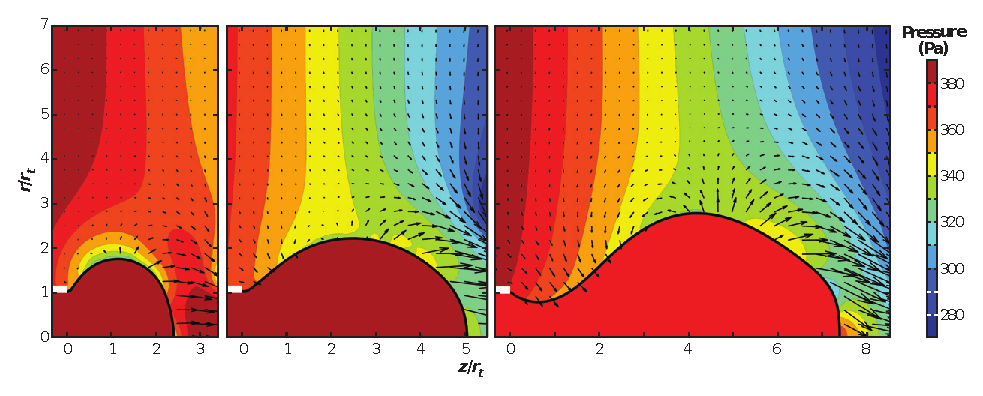
\includegraphics[width=\linewidth]{introduccion/figuras/esquemaBurbuja.eps}
\caption{Contornos de presión en las fases iniciales del proceso de formación de una burbuja para un número de Bond, $Bo = 0.245$. Cortesía de~\cite{Rodriguez-Rodriguez2015b}}
\LABFIG{esquemaBurbuja}
\end{figure}

Sintetizando una vez más las ideas expuestas en~\cite{Rodriguez-Rodriguez2015b}, el proceso de formación de una burbuja en una piscina en reposo puede esquematizarse en las siguientes etapas:

\begin{itemize}
\item En primer lugar, para satisfacer \EQ{continuidad}, el volumen de la burbuja debe aumentar, lo que provoca velocidades radiales en el líquido hacia fuera de la burbuja. 
\item La presión del gas en el interior de la burbuja es prácticamente uniforme, y debe adaptarse a la del líquido exterior en algún punto entre $z = 0$ (véase la \FIG{esquemaBurbuja}) y $z = 2R_{b}$, el cenit de la misma, supóngase en $z \sim R_{b}$. 
\item A medida que el radio de la burbuja aumenta, la punta de la burbuja se encuentra con una sobrepresión respecto al líquido exterior del orden de $\sim \rho g R_{b}$, lo que contribuye a que el gas acelere al líquido exterior, mientras que, en $z = 0$, es el líquido el que ejerce una sobrepresión sobre la base de la burbuja del orden de $\sim -\rho g R_{b}$, lo que conlleva que el líquido induzca velocidades hacia el interior de la burbuja. 
\end{itemize}

Por lo tanto, si nos ceñimos al caso no viscoso, la burbuja se desprenderá del inyector cuando la velocidad hacia adentro en $z = 0$, que surge del balance de \EQ{rayleighPlesset}, $\Delta p = p_{exit} - 2\sigma/R_{b} \sim \rho \dot{R}_{b}$ coincida con la velocidad hacia afuera impuesta por continuidad, $\sim Q_{g}/\left(4\pi R_{b}^{2}\right)$.

\begin{equation}\LABEQ{dbestimado}
\dfrac{Q_{g}}{R_{b}^{2}} \sim 	\sqrt{\dfrac{\Delta p}{\rho}} \sim \sqrt{g R_{b}} \Rightarrow d_{b} \sim \left(\dfrac{Q_{g}}{g^{1/2}}\right)^{2/5}
\end{equation}

siendo, finalmente, la frecuencia de producción 

\begin{equation}\LABEQ{fbestimado}
f_{b}\sim \dfrac{Q_{g}}{d_{b}^{3}} \sim	\left(\dfrac{g^{3}}{Q_{g}}\right)^{1/5}
\end{equation}

Así, aunque puede emplearse este sencillo método para producir burbujas simplemente inyectando gas en el seno de un líquido en reposo, la burbujas obtenidas poseen un diámetro significativamente mayor que el radio del inyector y con frecuencias que decrecen con el caudal, por lo que no resulta un método adecuado para satisfacer las demandas que las aplicaciones actuales requieren en lo que a diámetros y frecuencias se refiere\cite{Rodriguez-Rodriguez2015b}. Ello ha propiciado el desarrollo de tecnologías más sofisticadas basadas en dispositivos microfluídicos los cuales, en esencia, buscan aumentar el gradiente de presión (esto es, la gravedad efectiva) al que se ve sometida la gota en su proceso de generación. 




\section{Dispositivos para la generación de microburbujas}\LABSEC{tecnologias}


Una vez que se han descrito las ecuaciones necesarias para la compresión de los fundamentos de la generación de burbujas en el seno de un líquido, se está en disposición de enumerar y describir de forma sucinta las tecnologías más relevantes que, actualmente, se emplean para producir masivamente las mencionadas burbujas. Conviene recordar que las soluciones tecnológicas que aquí se presentan no son las únicas que permiten la producción de burbujas con tamaños submilimétricos; en efecto, en aplicaciones industriales como los reactores químicos, los esfuerzos de cortadura fruto de la turbulencia son los responsables de que la formación de burbujas que, aunque micrométricas y a grandes frecuencias, son generadas con un alto PDI~\cite{Rodriguez-Rodriguez2015b}.

De nuevo, al igual que se realizó en \SEC{fundamentos}, se respetará la estructura de~\cite{Rodriguez-Rodriguez2015b} para presentar las tecnologías que a continuación se describen, no extendiénsose en exceso y pudiendo encontrar el lector una descripción más detallada tanto en el \textit{review} como en las referencias citadas en él. Así pues, en la \FIG{tecnologias}, se describen de forma esquemática los dispositivos más relevantes para la producción de burbujas actualmente. En la figura se pueden distinguir dos tipos principales de tecnologías: aquellas emplean una corriente de líquido para provocar el colapso de la corriente gaseosa para la formación de burbujas (\FIG{tecnologias}a-d) y aquellas que en las que se emplean ultrasonidos (\FIG{tecnologias}e-f). A su vez, de entre las primeras, se puede distinguir en aquellas en las que el líquido es inyectado en la misma dirección que la corriente gaseosa (\FIG{tecnologias}a-c) y aquellas en las que el líquido y el gas se encuentran de forma perpendicular (\FIG{tecnologias}d). Finalmente, la diferencia principal entre los dispositivos de \emph{flow-focussing} (\FIG{tecnologias}b-c), y los de \emph{coflow} es que en el primero se hace pasar ambos fluidos a través de un estrechamiento, lo que acelera colapso y permite generar burbujas más pequeñas~\cite{Rodriguez-Rodriguez2015b}. En esta sección, nos centraremos sólo en los 4 primeros, debido a la analogía que los mismos presentan con la solución tecnológica de la que trata este estudio. 


\begin{figure}
\LABFIG{tecnologias}
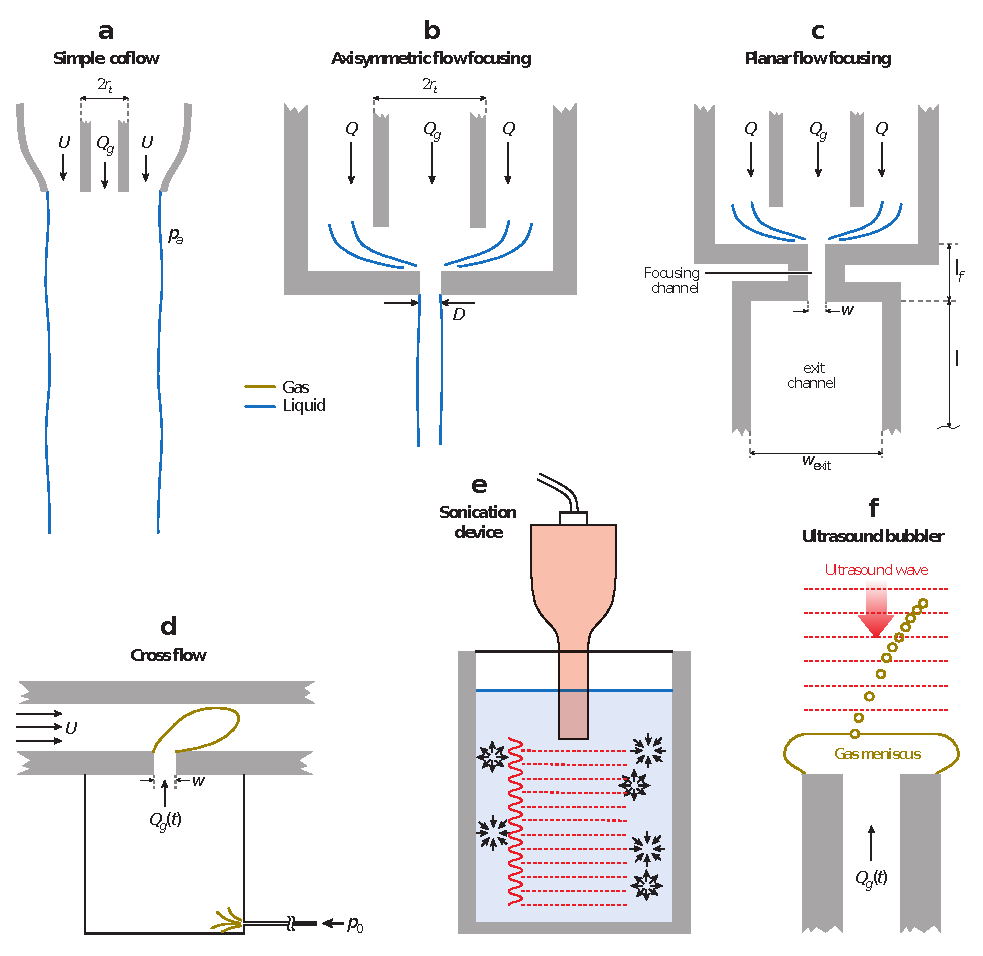
\includegraphics[scale=1]{introduccion/figuras/tecnologias.eps}
\caption{Representación esquemática de los diferentes dispositivos que identiican la tecnología utilizada en la producción de burbujas monodispersas. Figura adaptada de~\cite{Rodriguez-Rodriguez2015b}.}
\LABFIG{tecnologias}
\end{figure}

\subsection{Dispositivos de Coflow}\LABSSEC{coflow}

Un dispositivo de tipo coflow es aquél como el mostrado en la \FIG{tecnologias}a, donde la corriente gaseosa y la de líquido son inyectadas en la misma dirección y de forma libre. Las condiciones en las que usualmente se opera este tipo de dispositivos son aquellas en las que el número de Reynolds y Webber son tales que $Re = \rho U r_{t}/\mu \gg 1$ y $We = \rho U^{2} r_{t}/ \sigma$. Bajo estas condiciones, las frecuencias de producción, $f_{b}$ y los diámetros equivalentes de las burbujas obtenidas, $d_{b} = \left[\left(6Q_{g}\right)/\left(\pi f_{b}\right)\right]^{\left(1/3\right)} $, dependen sólo del ratio de velocidades gas-líquido, $U_{g}/U$, y del ratio $r_{t}/U$. Además, en los casos bajo consideración donde $We \gg 1$, el líquido exterior impone la velocidad a la que la interfase es transportada, con lo que se previene la coalescencia ya que las burbujas son transportadas a la velocidad del líquido~\cite{Sevilla2005a}. Precisamente, en una operación normal con este tipo de dispositivos, la velocidad del gas suele ser mayor que la del líquido, con lo que las burbujas son generadas cerca de la punta del inyector. Siguiendo las mismas ideas que el proceso basado en las fases de expansión y posterior colapso descrito en \SEC{fundamentos}, en \cite{Gordillo2007a} se desarrolla un modelo simple para la fase de colapso en el que puede comprobarse que, en el límite en el que $U_{g}/U \gg 1$, la frecuencia escala como $f_{b}\simeq 0.15U/r_{t}$. 

Por otro lado, el caso contrario en el que $Re \ll 1$ no ha sido muy reportado en la literatura~\cite{Rodriguez-Rodriguez2015b}. En este caso, en lugar del número de Webber, el parámetro adimensional que gobierna el problema es el número capilar, $Ca = \mu U /\sigma$, además del ratio $U_{g}/U$ como en el caso anterior y del ya descrito número de Bond, $Bo$. En este caso, tras el exhaustivo estudio numérico de~\cite{Suryo2006a}, se tiene que el diámetro de las burbujas decrece cuando el ratio $U_{g}/U$ también lo hace. 

\subsection{Dispositivos de Cross-Flow}\LABSSEC{crossflow}

Los dispositivos de tipo Cross-Flow son aquellos como los mostrados en la \FIG{tecnologias}d, donde puede apreciarse que el gas es inyectado de forma perpendicular al líquido a través de una junta en T. Para tener buen control y repetibilidad en los tamaños de las burbujas, estos dispositivos operan a números de Reynolds muy bajos, por lo que su mayor campo de amplicación se encuentra dentro de la microfluídica. Dado que operan a $Re \ll 1$, se observan diferentes regímenes en función del número capilar, $Ca$, como son el \emph{squeezing, dripping} o \emph{jetting}. De entre ellos, el que parece más apropiado para el control del diámetro de las burbujas es el \emph{squeezing}, lo que ocurre cuando $Ca \lesssim \\mathcal{O}\left(10^{-2}\right)$. Por otro lado, una de las principales desventajas del empleo de este tipo de dispositivo es la baja frecuencia de producción derivada de la operación a bajos números capilares. En efecto, si se pretende aumentar la velocidad del líquido para aumentar dicha frecuencia, también se producirá un aumento del numero capilar, lo que limita en general la frecuencia de producción de estos dispositivos a $f_{b}\sim 10^{3} \mathrm{Hz}$. 

Tanto los dispositivos con configuraciones de tipo Cross.Flow como los de Coflow permiten tener control de forma separada del diámetro de las burbujas y de su frecuencia, variando $Q_{g}$ y $Q$. Sin embargo, a pesar de ser dispositivos microfluídicos de tamaños del orden de las centenas de milímetros (o mayores), su geometría limita el tamaño mínimo de las burbujas que se pueden obtener. Esta dificultad puede ser superada e través de otro método conocido como \emph{Flow-Focussing} que utiliza una geometría un tanto diferente como se verá en la próxima subsección. 

\subsection{Dispositivos de Flow-Focussing}\LABSSEC{flowfocussing}


La sencillez de los dispositivos descritos anteriormente posee un notable inconveniente, pues si se elmina la inyección de gas las líneas de líquido son casi paralelas, con lo que los gradientes de presión existentes son prácticamente despreciables~\cite{Rodriguez-Rodriguez2015b}. La demanda de diámetros cada vez menores de las burbujas hace que sea tecnológicamente inviable reducir tanto como se desee el diámetro del inyector, por lo que otras soluciones han emergido para paliar las limitaciones de las configuraciones de coflow y crossflow; una de ellas, es el empleo de dispositivos de \emph{Flow-Focussing}. En geometrías de flow-focussing como las mostradas en la \FIG{tecnologias}b-c, la presencia del estrechamiento provoca (además de un coflujo de líquido y gas que previene la aparición de coalescencia) un gradiente longitudinal de presión, cuyo efecto principal es el de reducir el diámetro final de las burbujas obtenidas. Los primeros en reportar este fenómeno fueron~\cite{Ganan-Calvo2001a}, obteniendo burbujas de tamaños $d_{b} \mathcal{O}\left(10 \mu m\right) < D$, controlando simplemente el ratio $Q_{g}/Q$  y el caudal de líquido exterior $Q = \pi D^{2} U/4$, con $D$ el diámetro del estrechamiento. En efecto, el papel del gradiente axial de presión es análogo al jugado por la gravedad en el caso de la \EQ{dbestimado}, esto es, tomando $\Delta p_{exit} = \nabla p R_{b}$, y teniendo en cuenta que el gradiente de presión puede ser obtenido de forma estimada de las ecuaciones de Navier-Stokes como

\begin{equation}\LABEQ{focusGradPres}
\rho \dfrac{D\mathbf{u}}{Dt} = -\nabla p \Rightarrow \nabla p \sim \rho \mathbf{u} \cdot \nabla \mathbf{u} \sim \rho U^{2}/D
\end{equation}

se tiene, sustituyendo $ \Delta p $ en \eqref{eq:dbestimado},

\begin{equation}\LABEQ{focusDbEstimado}
\dfrac{d_{b}}{D} \sim \left(\dfrac{Q_{g}}{Q}\right)^{2/5}
\end{equation}

siendo pues la frecuencia de burbujeo 

\begin{equation}\LABEQ{focusFb}
f_{b} = \dfrac{6 Q_{g}}{\pi d_{b}^{3}} \propto \dfrac{U}{D}\left(\dfrac{Q_{g}}{Q}\right)^{-1/5}
\end{equation}

por lo que este dispositivo también permite controlar de forma separada tamaño y frecuencia de producción simplemente a través de la variación de los reatios $Q_{g}/Q$ y de la velocidad del líquido $U$. Uno de los principales escollos en el uso de este tipo de dispositivos se encuentra en la dificultad que supone conseguir un buen alineamiento entre los diferentes canales, lo que introdujo la configuración de la \FIG{tecnologias}c, que permite simplificar esta labor.


\subsection{Otros dispositivos y breve reflexión}\LABSSEC{ConclusionDevices}

Existe, además de los descritos en los apartados anteriores, otros dispositivos para generar burubujas de tamaño micrométrico de forma monodispersa, como son aquellos basados en la aplicación de ondas acústicas, tal y como se muestra en la \FIG{tecnologias}e-f, y lo que es más, nada impediría (en principio) combinar estos dispositivos con los anteriores, si se pretende reducir aún ás el diámetro de las burbujas~\cite{Rodriguez-Rodriguez2015b}. A través de los ejemplos más significativos de dispositivos que aquí se han presentado, el lector puede estimar que el tamaño característico de estos dispositivos se encontrará en un rango comprendido entre $\sim \mathcal{O}(10 \mu\, m)$ hasta  $\sim \mathcal{O}\left(10 \,\mathrm{mm}\right)$, lo que a priori puede suponer una dificultad tanto de fabricación como de operación; además, a la dificultad de manejo de los instrumentos microfluídicos habría que sumar la limitación existente en la frecuencia máxima de producción, que estaría limitada por el tamaño de los dispositivos y cuya solución se encontraría en la fabriación de un número mayor de estos. Cabe entonces preguntarse si los mecanismos físicos ya descritos y que subyacen bajo los diferentes procesos de producción de microburbujas aquí presentados van aparajados necesariamente del empleo de dispositivos microfluídicos. En efecto, si bien a lo largo del capítulo se ha podido comprobar que existe una clara dependencia con el diámetro del inyector del gas (lo que apoya la necesidad del empleo de la microfluídica), también es cierto que las condiciones de contorno que el líquido exterior impone sobre la corriente gaseosa, bien únicamente mediante el transporte a la velocidad del líquido de la interfase (coflow y cross-flow) o bien sumando el gradiente longitudinal de presión provocado por un estrechamiento (flow-focussing), no tendrían (en principio) porqué ir ligadas taxativamente al empleo de geometrías micrométricas.  

Así pues, en la siguiente sección de este capítulo se discute con más detalle el papel que el gradiente de presión juega en la formación de burbujas, prestando especial atención para ello en una técnica conocida como \emph{Confined-Selective-Withdrawal} que presenta características comunes tanto a las configuraciones de coflow y flow-focussing. Se pretende así reforzar la idea de la importancia que juega el gradiente de presión en la formación de burbujas para, finalmente, plantear si cabría la posibilidad de plantearse un dispositivo capaz de generar microburbujas monodispersas de forma masiva con dimensiones características mucho mayores que las de los dispositivos empleados actualmente. 

\section{Influencia del gradiente de presión}\LABSEC{gradPres}

A lo largo de la \SEC{tecnologías}, se ha podido comprobar como el papel del líquido exterior en la generación de microburbujas puede ir desde simplemente imponer la velocidad de la entrefase previniendo la coalescencia hasta ejerecer un efecto análogo al de la gravedad a través del gradiente axial de presión. Las conclusiones extraídas en la \SSEC{ConclusionDevices} motivan indagar un poco más en el papel que dicho gradiente longitudinal de presión puede jugar en el proceso de formación de burbujas, por lo que se van a presentar de forma sucinta los resultados obtenidos~\cite{Evangelio2015b} donde se obtuvieron burbujas de tamaño micrométrico empleando la técnica conocida como \emph{Confined Selective Withdrawal}.

\begin{figure}[hbtp!]
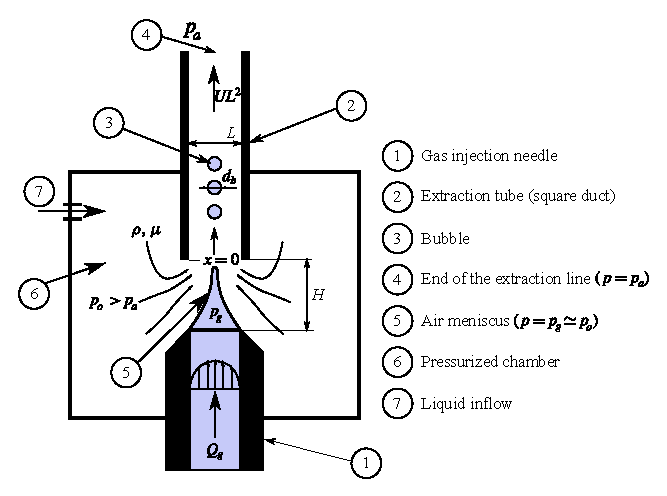
\includegraphics[scale=1]{introduccion/figuras/esquemaCSW.eps}
\caption{Esquema del dispositivo empleado en~\cite{Evangelio2015b} para la producción de microburbujas con la técnica de Confined Selective Withdrawal. Imagen adaptada de~\cite{Evangelio2015b}}
\LABFIG{esquemaCSW}
\end{figure}

 En la \FIG{esquemaCSW} se describe esquemáticamente el funcionamiento de este dispositivo. El dispositivo consiste en cámara presurizada a $p_{0}$ con un líquido, de densidad $\rho$ y de viscosidad $\mu$, que se suministra desde el exterior y que descarga a $p_{a} < p_{0}$ a través de una salida a través de un capilar (en este caso de sección cuadrada) de dimensiones características $L = 1\,\mathrm{mm}$. El capilar se encuentra perfectamente alineado con una aguja donde se inyecta el gas con caudal $Q_{g}$ y que se encuentra a una distancia $H$ del capilar. Como puede observarse en la \FIG{fenomenologia}, para velocidades del líquido en el capilar inferiores a una $U < U^{*}$, el menisco emite burbujas de forma pulsante y de diferentes diámetros~\cite{Evangelio2015b}. Sin embargo, por encima de esta velocidad, se puede observar que el menisco de aire se mantiene estable para una regíon $x \leq x_{s}$, lo que propicia la aparición de un régimen de producción de burbujas monodispersas; la condición de equilibrio de la que resulta $x_{s}$ será discutida más adelante. Finalmente, en la \FIG{produccionEstable} se muestra como, para valores de $U > U^{*}$, aguas abajo de la zona estacionaria ($x \leq x_{s}$), se produce un cilindro de gas de diámetro $d_{g}$ y longitud $\ell$ que, finalmente, culmina con la producción de una nueva burbuja; una vez la burbuja es emitida y transportada a la velocidad del líquido, se inicia nuevamente el proceso de formación de otra burbuja a través del mecanismo descrito. 
 
\begin{figure}[hbtp!]
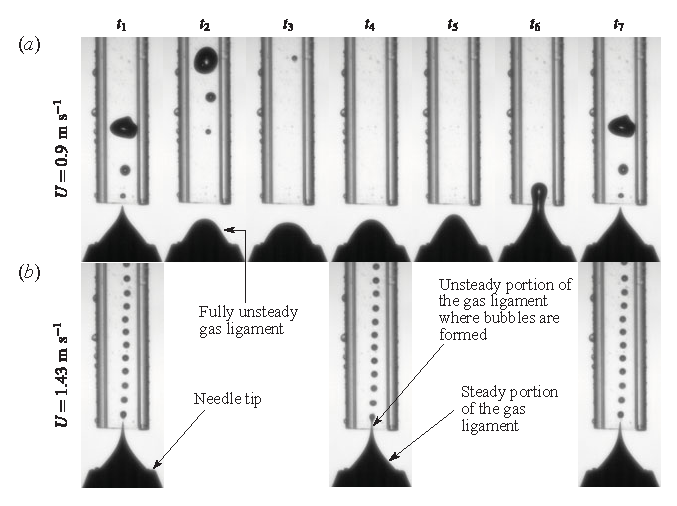
\includegraphics[scale=1]{introduccion/figuras/fenomenologia.eps}
\caption{Diferentes regímenes de burbujeo en función de la velocidad $U$ a la que el líquido circula a través del capilar. En (a) se visualiza el caso en que $U < U^{*}$, por lo que no se tiene un régimen de burbujeo constante, mientras que en (b), $U > U^{*}$, se consigue alcanzar un régimen de producción de burbujas monodispersas. Imágenes adaptadas de~\cite{Evangelio2015b}.}
\LABFIG{fenomenologia}
\end{figure}

Aunque en~\cite{Evangelio2015b} se analiza tanto el caso viscoso como el no viscoso, en esta sección nos centraremos únicamente en los casos $Re \gg 1$, ya que será el caso de interés para el dispositivo que aquí se describe. Antes de comenzar el análisis, conviene notar que la presión del gas, $p_{g}$, que además se considera constante a lo largo del mismo según la hipótesis ya comentada en la \SEC{fundamentos}, debe de encontrarse en equilibrio con la del líquido a la salida de la aguja, donde la velocidad del líquido es casi nula, por lo que puede suponerse que $p_{g} \simeq p_{0}$. Así, para obtener un menisco de aire estable en la región $x \leq x_{s}$, la diferencia de presiones $p_{0} - p\left(x\right)$ debe estar en equilibrio con la presión capilar. En efecto, considerando que el hilo gaseoso tenga un diámetro $d_{g}$, llamando $U_{0}$ a la velocidad en el centro del tubo capilar, y teniendo en cuenta el cumplimiento de la ecuación de continuidad

\begin{equation}
Q_{g} = \dfrac{\pi d_{g}^{2}}{4}U_{0} \Rightarrow d_{g} \sim \left(\dfrac{Q_{g}}{U_{0}}\right)^{1/2}
\LABEQ{continuidadLigamento}, 
\end{equation}

se tiene que 

\begin{equation}
p_{0} - p\left(x_{s}\right) = \dfrac{2\sigma}{d_{g}} \simeq \dfrac{2\sigma}{\left(Q_{g}/U_{0}\right)^{1/2}}
\LABEQ{equilibrioLigamento}
\end{equation}

lo que proporciona la condición de equilibrio para que exista un menisco de aire estacionario en $x \leq x_{s}$. Tanto en \eqref{eq:contiuidadLigamento} como en \eqref{equilibrioLigamento}, la expresión de $U_{0}$ vendrá determinada por el tipo de flujo que exista en el capilar, lo que para el caso en el que $Re \gg 1$ y teniendo en cuenta los resultados de las simulaciones
\footnote{En~\cite{Evangelio2015b} se realiza una simulación del dominio considerando este como axilsimétrico y sin simular la fase gaseosa, lo que suele realizarse generalmente cuando se desea estudiar la estabilidad de chorros, descomponiendo el campo de presiones como suma de la solución básica más una perturbación (véase como ejemplo~\cite{Gordillo2014a}. En~\cite{Evangelio2015b}, sin embargo, se realiza la hipótesis, verificada \textit{a posteriori}, de que la presencia de las burbujas no perturba el campo de presiones del líquido.} realizadas en~\cite{Evangelio2015b} constituye un perfil uniforme de velocidad; efectivamente, este hecho queda representado por el valor del coeficiente de presión adimensional $\xi = \left(p_{0} - p\left(x\right)\right)/\left(1/2 \rho U^{2}\right) \simeq 1$ en $x = 0$. Así, dado que $p_{0} - p\left(x_{s}\right) \sim 1/2\rho U^{2}$ para $Re \gg 1$ y teniendo en cuenta que la formación de burbujas tnedrá lugar si $p_{0}-p\left(x\right) > \dfrac{2\sigma}{d_{g}}$, la formación de burbujas monodispersas será posible si 

\begin{equation}
\beta = \dfrac{\rho U^{2} L}{4\sigma}q^{1/2} \gtrsim 1 \qquad \mathrm{con} q = \dfrac{Q_{g}}{UL^{2}}
\LABEQ{beta}
\end{equation}

donde $\beta$ en la \EQ{beta} constituye un parámetro similar al número de Webber, $We = \rho U^{2}L^{2}/\sigma$; la validez de \eqref{eq:beta} queda mostrada en~\cite{Evangelio2015b}.

\begin{figure}[hbtp!]
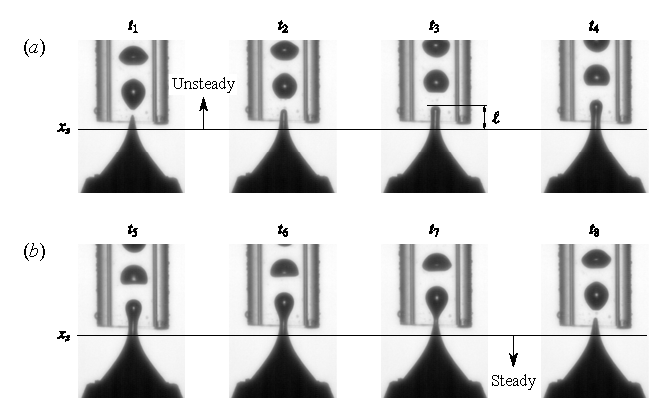
\includegraphics[scale=1]{introduccion/figuras/produccionEstable.eps}
\caption{Secuencia de producción de burbujas a partir de un menisco de aire estable para la región $x \leq x_{s}$. Como se aprecia en la figura, aguas abajo de $x_{s}$, se emite un cilindro de gas de diámetro $\sim d_{g}$ que se extiende una longitud $\ell$. Imagen tomada de~\cite{Evangelio2015b}.}
\LABFIG{produccionEstable}
\end{figure}


Una vez se han descrito las condiciones neesarias para la producción monodispersa de burbujas y se conocen las condiciones de equilibrio estacionario del menisco de aire, se está en condición de describir el resto del proceso de formación, así como las expresiones de los diámetros y frecuencias de producción de las burbujas obtenidas. Una vez que las burbujas se desprenden del ligamento de gas en $Lx \approx Lx_{s} + \ell$, la diferencia de presión $\Delta p = p_{0} - p\left(x\right) -2\sigma/d_{g} > 0$, induce velocidades radiales sobre el ligamento de gas que provoca el inicio del proceso de formación de una nueva burbuja. Dado que durante los instantes posteriores a la eyección de una nueva burbuja el diámetro del cilindro apenas varía, es posible escribir

\begin{equation}
\begin{split}
&\Delta p = p_{0} - p\left(x\right) - 2\sigma/d_{g} = p_{0} - p\left(x_{s}\right) - 2\sigma/d_{g} + p\left(x_{s}\right) - p\left(x\right) \approx \\
& \approx - \dfrac{\mathrm{d}p}{\mathrm{d} x}\left(x_{s}\right)\left(x-x_{s}\right) \approx \dfrac{\mathrm{d}\left(p_{0}-p\right)}{\mathrm{d}x}\left(x_{s}\right)\dfrac{\ell}{L}
\end{split}
\LABEQ{gradPress}
\end{equation}

donde se ha tenido en cuenta la \EQ{equilibrioLigamento} y se ha realizado un desarrollo en serie de Taylor de primer orden de la presión en torno al punto $x = x_{s}$. De este modo, y tal y como se detalla en~\cite{Evangelio2015b}, la \EQ{gradPress} muestra como el proceso de formación de burbujas está gobernado por el gradiente de presión local en el punto $x = x_{s}$, por lo que, como ya se ha comentado previamente, el gradiente de presión local posee un papel absolutamente análogo al que tiene la gravedad en la formación de una burbuja en una piscina en reposo. Por lo tanto, siguiendo el procedimiento que se siguió en la \SEC{fundamentos}, si se sustituye la \EQ{gradPress}, particularizada para el caso $Re \gg 1$, en la ecuación de Rayleigh-Plesset (\EQ{rayleighPlesset}), se tendrá que 

\begin{equation}
\rho R_{b}\ddot{R}_{b} \propto \dfrac{\mathrm{d}\left(p_{0} - p\right)}{\mathrm{d}x}\left(x_{s}\right)\dfrac{\ell}{L}\propto \dfrac{\ell}{2L}\rho U^{2} P_{s}
\end{equation}

siendo $P_{s} = \dot{\xi}\left(x_{s}\right)$. La ecuación anterior junto con la ecuación de continuidad~\eqref{eq:continuidad}, reescrita aquí por conveniencia

\begin{equation}
Q_{g} = \dfrac{\pi}{6}d_{b}^{3} f_{b}
\end{equation}

permiten obtener las frecuencias de producción,

\begin{equation}
\rho \dfrac{P_{s}}{2}\dfrac{U^{2}}{L}\ell \propto \rho R_{b} \ddot{R}_{b} \sim \rho d_{b}^{2}f_{b}^{2} \Rightarrow f_{b} \propto \dfrac{U\sqrt{P_{s}/2}}{\sqrt{L d_{b}}}\sqrt{\dfrac{\ell}{d_{b}}}
\LABEQ{freqGradPres}
\end{equation}

y, finalmente, tomando $\ell \propto d_{b}$ empleando la analogía al caso de formación de burbujas en una piscina en reposo~\cite{Evangelio2015b}, la expresión final de la frecuencia y los diámetros de las burbujas. 

\begin{equation}
f_{b} \propto \dfrac{U\sqrt{P_{s}/2}}{\sqrt{L d_{b}}} \quad \mathrm{y} \quad \dfrac{d_{b}}{L} \propto \left(\dfrac{Q_{g}}{U\sqrt{P_{s}/2}L^{2}}\right)^{2/5}
\end{equation}

El proceso seguido para la obtención de las ecuaciones~\eqref{eq:freqGradPres} y \eqref{dbGradPres} es completamente análogo al descrito en la \SEC{fundamentos} con el gradiente de presión local ejerciendo el papel de la gravedad y con la diferencia que $\rho U^{2}/L \gg \rho g $, lo que atendiendo a las ecuaciones de arriba, se traduce en un aumento de la frecuencia y una disminución de los diámetros obtenidos. Este hecho invita a pensar que, si el proceso de formación descrito está controlado por el gradiente de presión local en $x_{s}$, nada impide imaginar dispositivos generadores de burbujas donde los gradientes favorables de presión puedan obtenerse con geometrías tan diversas como diferentes a la descrita en~\cite{Evangelio2015b}.


\section{Analogía Aerodinámica}\LABSEC{aerodynamics}

Al final de La \SEC{gradPres}, basándose en las ideas de~\cite{Evangelio2015b}, se dejó entrever la posibilidad de obtener gradientes favorables de presión similares a los encontrados en dispositivos de Confned Selective Withdrawal o Flow-Focussing pero con otras geometrías completamente diferentes. La motivación en la exploración de otras geometrías es doble: dispositivos con tamaños alejados de la escala de la microfluídica permitirían no sólo una fabricación y operación más sencilla sino también aumentar notablemente las frecuencias de producción de las burbujas. Así, un ejemplo cotidiano de geometrías donde se producen fuertes gradientes favorables de presión lo constituyen los perfiles aerodinámicos empleados como sección transversal en las alas de los aviones. Dado que la única premisa que, \textit{a priori}, debe cumplir una geometría alternativa a las empleadas actualmente sería conseguir gradientes de presión comparables a los creados en los dispositivos microfluídicos, ¿qué impide pensar que se pueda emplear un ala para producir masivamente microburbujas monodispersas?

Conviene antes de seguir, no obstante, esbozar algunas ideas básicas en aerodinámica que permitirán comprender mejor la posibilidad de emplear un ala como dispositivo generador de burbujas. La Aerodinámica es la parte de la Mecánica de Fluidos que se encarga del estudio del movimiento de gases (generalmente aire) alrededor de un cuerpo. Teniendo en cuenta las propiedades del aire (densidad $\rho_{g} \sim \mathcal{O}(1\,\mathrm{kg/m^{3}})$ y viscosidad $\mu \sim \mathcal{O}(10^{-5}\,\mathrm{Pa \cdot s})$ a $T = 20^{\circ}$) y las velocidades características de un cuerpo que se mueve en él (tómese como ejemplo un coche circulando a $V = 30\,\mathrm{m/s} $ o el ala de un avión a $V = 100\, \mathrm{m/s}$) se tiene que los números de Reynolds característicos del flujo de aire alrededor de un objeto con dimensiones características $L = 1\,\mathrm{m}$ serán $Re = \rho V L / \mu  \sim \mathcal{O}\left(10^{6}\right)$. Bajo estas condiciones los efectos viscosos pueden ser despreciados en la mayor parte del dominio del problema salvo en una delgada región adyacente a la superficie del cuerpo (capa límite), donde la viscosidad impone la condición de contorno de velocidad relativa nula para el fluido con respecto al sólido y donde, por lo tanto, los efectos de inercia y los viscosos son del mismo orden ($Re \approx 1$); el espesor de esta capa puede ser estimado como $\delta_{L} \sim L Re^{-1/2}$, por lo que para el caso del ala de un avión ($L \sim 1\,\mathrm{m}$) esta capa tiene un espesor de apróximadamente 1\,mm. Sin embargo, la importancia de esta delgada capa en la estabilidad del flujo alrededor del cuerpo es capital, ya que si sus efectos no estuvieran confinados a la mencionada región la hipótesis de viscosidad despreciable en el resto del dominio no sería asumible. En efecto, si la corriente experimenta un gradiente adverso de presión (como el que experimenta un fluido cuando circula a través de un canal que se ensancha o el que pueda existir en una esfera aguas abajo del punto más alto de la misma), las velocidades cerca de la pared del sólido son tan cercanas a cero que puede producirse una recirculación del fluido, lo que provocaría el desprendimiento de la capa límite. Para que esto no se produzca, se puede reducir el gradiente desfavorable de presión extediendo la longitud del cuerpo aguas abajo del punto de mínima presión, lo que para el caso de un sólido en el seno del aire significaría emplear cuerpos fuselados (cuerpos con longitud transversal característica mucho menor que la longitudinal) en lugar de cuerpos romos (como sería por ejemplo una esfera). Además, para que la corriente no se desprenda, el ángulo con el que incide la corriente con respecto a línea media longitudinal del sólido, no debe ser muy elevado, ya que de lo contrario el desprendimiento también tendrá lugar. 

\begin{figure}[hbtp!]
\centering
\subfloat[Campo de presión y geometría]{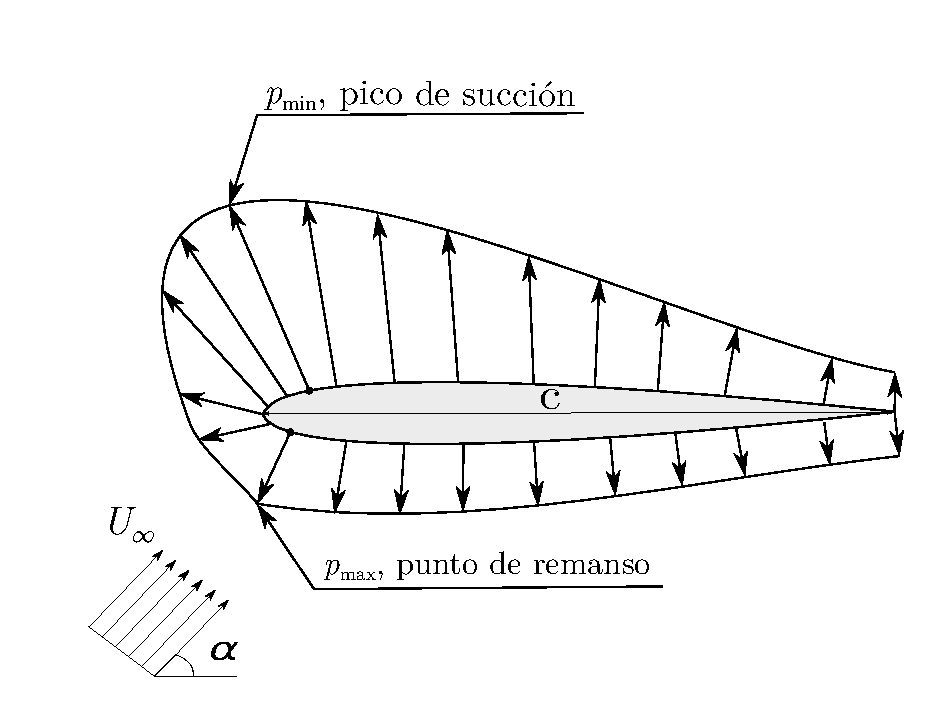
\includegraphics[width=.45\textwidth]{introduccion/figuras/airfoil.eps}\LABFIG{airfoil}}
\subfloat[Líneas de corriente]{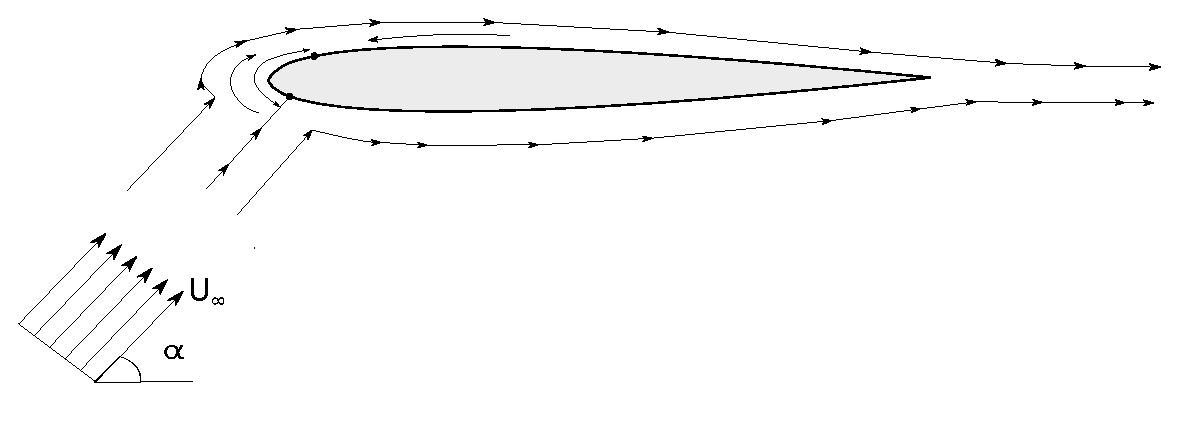
\includegraphics[width=.45\textwidth]{introduccion/figuras/streamlines.eps}\LABFIG{streamlines}}
\caption{Representación esquemática de un perfil aerodinámico que enfrenta una corriente a la velocidad $U_{\infty} $ que forma un ángulo de ataque $\alpha$ con la cuerda, $c$, del perfil. En la \FIG{airfoil} se representan el campo de presión cambiado de signo ($-(p(\mathbf{x})-p_{\infty})$, con $\mathbf{x}\in \Sigma_{s}$, indicando  tanto el pico de succión (punto de mínima presión) como el punto de remanso (punto de máxima presión). En la \FIG{streamlines} se muestra una representación cualitativa de las líneas de corriente alrededor de un perfil aerodinámico. Adicionalmente se representan las zonas de fuertes gradientes favorables de presión, esto es la zona que, conteniendo el borde de ataque, se extiende desde el punto de remanso hasta el pico de succión, y la zona de gradiente desfavorable de presión, que se extiende aguas abajo del pico de succión y que se ha representado con una flecha indicando el sentido de la recirculación que podría producirse en la capa límite.}
\end{figure}

En la \FIG{airfoil} se representa de forma esquemática un perfil aerodinámico que enfrenta una corriente a la velocidad $U_{\infty}$ que forma con la \emph{cuerda del perfil}, $c$, un \emph{ángulo de ataque}, $\alpha$. Considerando que el flujo incidente es uniforme y carente de vorticidad (esto es $\omega = \nabla \times \mathbf{v} = 0$) y despreciando los efectos viscosos en todo el dominio excepto en la capa límite, la velocidad deriva de un potencial, $\mathbf{v} = \nabla \phi$, por lo que, imponiendo la ecuación de continuidad se llega al siguiente problema de contorno

\begin{eqnarray}
\nabla^{2} \phi & = & 0 \\
\nabla \phi \cdot \mathbf{n} & = & 0, \quad \mathbf{x} \in \Sigma_{s}\\
\left|\nabla \phi \right| & \rightarrow & 0, \quad \left|\mathbf{x}\right| \rightarrow \infty
\LABEQ{problemaContorno}
\end{eqnarray}


Con las hipótesis realizadas, la resolución de este problema arroja resultados cualitativos y cuantitativos que ayudarán a comprender mejor el campo de velocidades y en especial de presiones del fluido alrededor del perfil. El problema de la laplaciana, que puede ser resuleto con un método de elementos de cotorno%INCLUIR SI DA TIEMPO UN APÉNDICE CON EL MÉTODO EMPLEADO!!!!!!
, normalmente se descompone como $\phi = \phi_{\infty} + \phi'$, siendo $\phi_{\infty}$ el potencial correspondiente a una corriente infinita a ángulo de ataque $\alpha$ y $\phi^{'}$ el potencial de perturbación causado por la presencia del perfil. En la \FIG{resultadoPotencial} se muestran los resultados de una simulación realizada con el método de los elementos de contorno para problemas bidimensionales aplicada a un perfil simétrico NACA~0012 que se mueve en el seno de un fluido a un ángulo de ataque $\alpha = 4^{\circ}$. Como se puede observar en la \FIG{upotencial} y más detalladamente en la \FIG{upotencialZoom}, la velocidad longitudinal de perturbación posee un mínimo que se corresponde con el punto de remanso (punto de máxima presión) en la \FIG{cp}; nótese que, por conveniencia, se representa el \emph{coeficiente de presión}, $C_{p} = \left(p-p_{\infty}\right)/\left(1/2\rho U_{\infty}^{2}\right)$, cambiado de signo. Del mismo modo, el máximo de $u'$ se corresponde con el punto de mínima presión (pico de succión) como se muestra en la \FIG{cp} y más detalladamente en la \FIG{cpZoom}. 


\begin{figure}
\centering
\subfloat[Velocidad de perturbación adimensional $u'/U_{\infty}$]{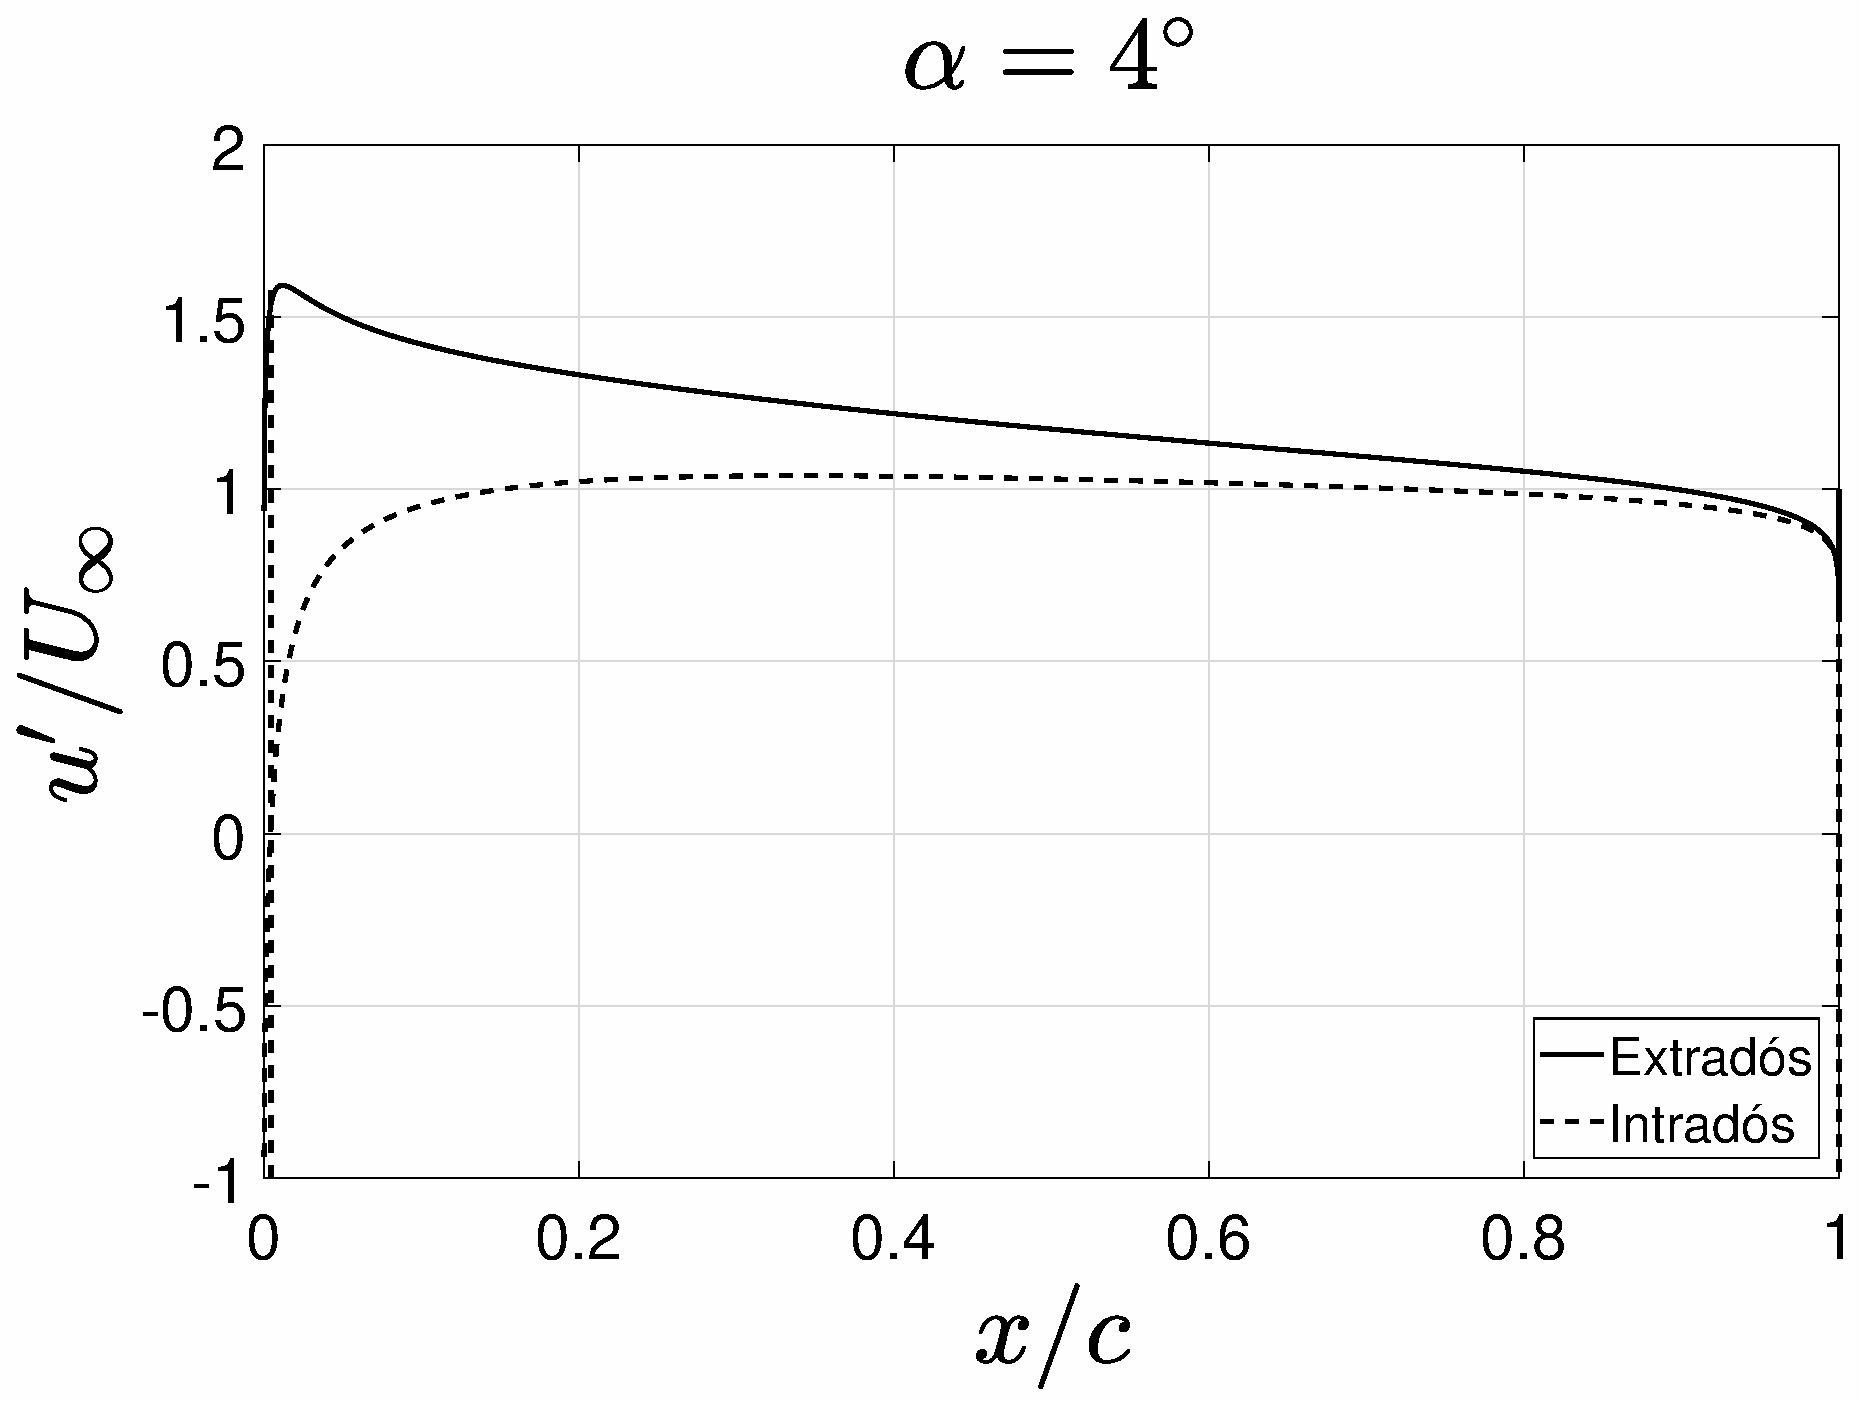
\includegraphics[width = .45\textwidth]{upotencial.eps}\LABFIG{upotencial}}
\subfloat[Zoom de $u'/U_{\infty}$ en el borde de ataque]{\includegraphics[width = .45\textwidth]{uptonecialZoom.eps}\LABFIG{upotencialZoom}} \\
\subfloat[Representación de $-C_{p} = -\left(p-p_{\infty}\right)/\left(1/2\rho U_{\infty}^{2}\right)$]{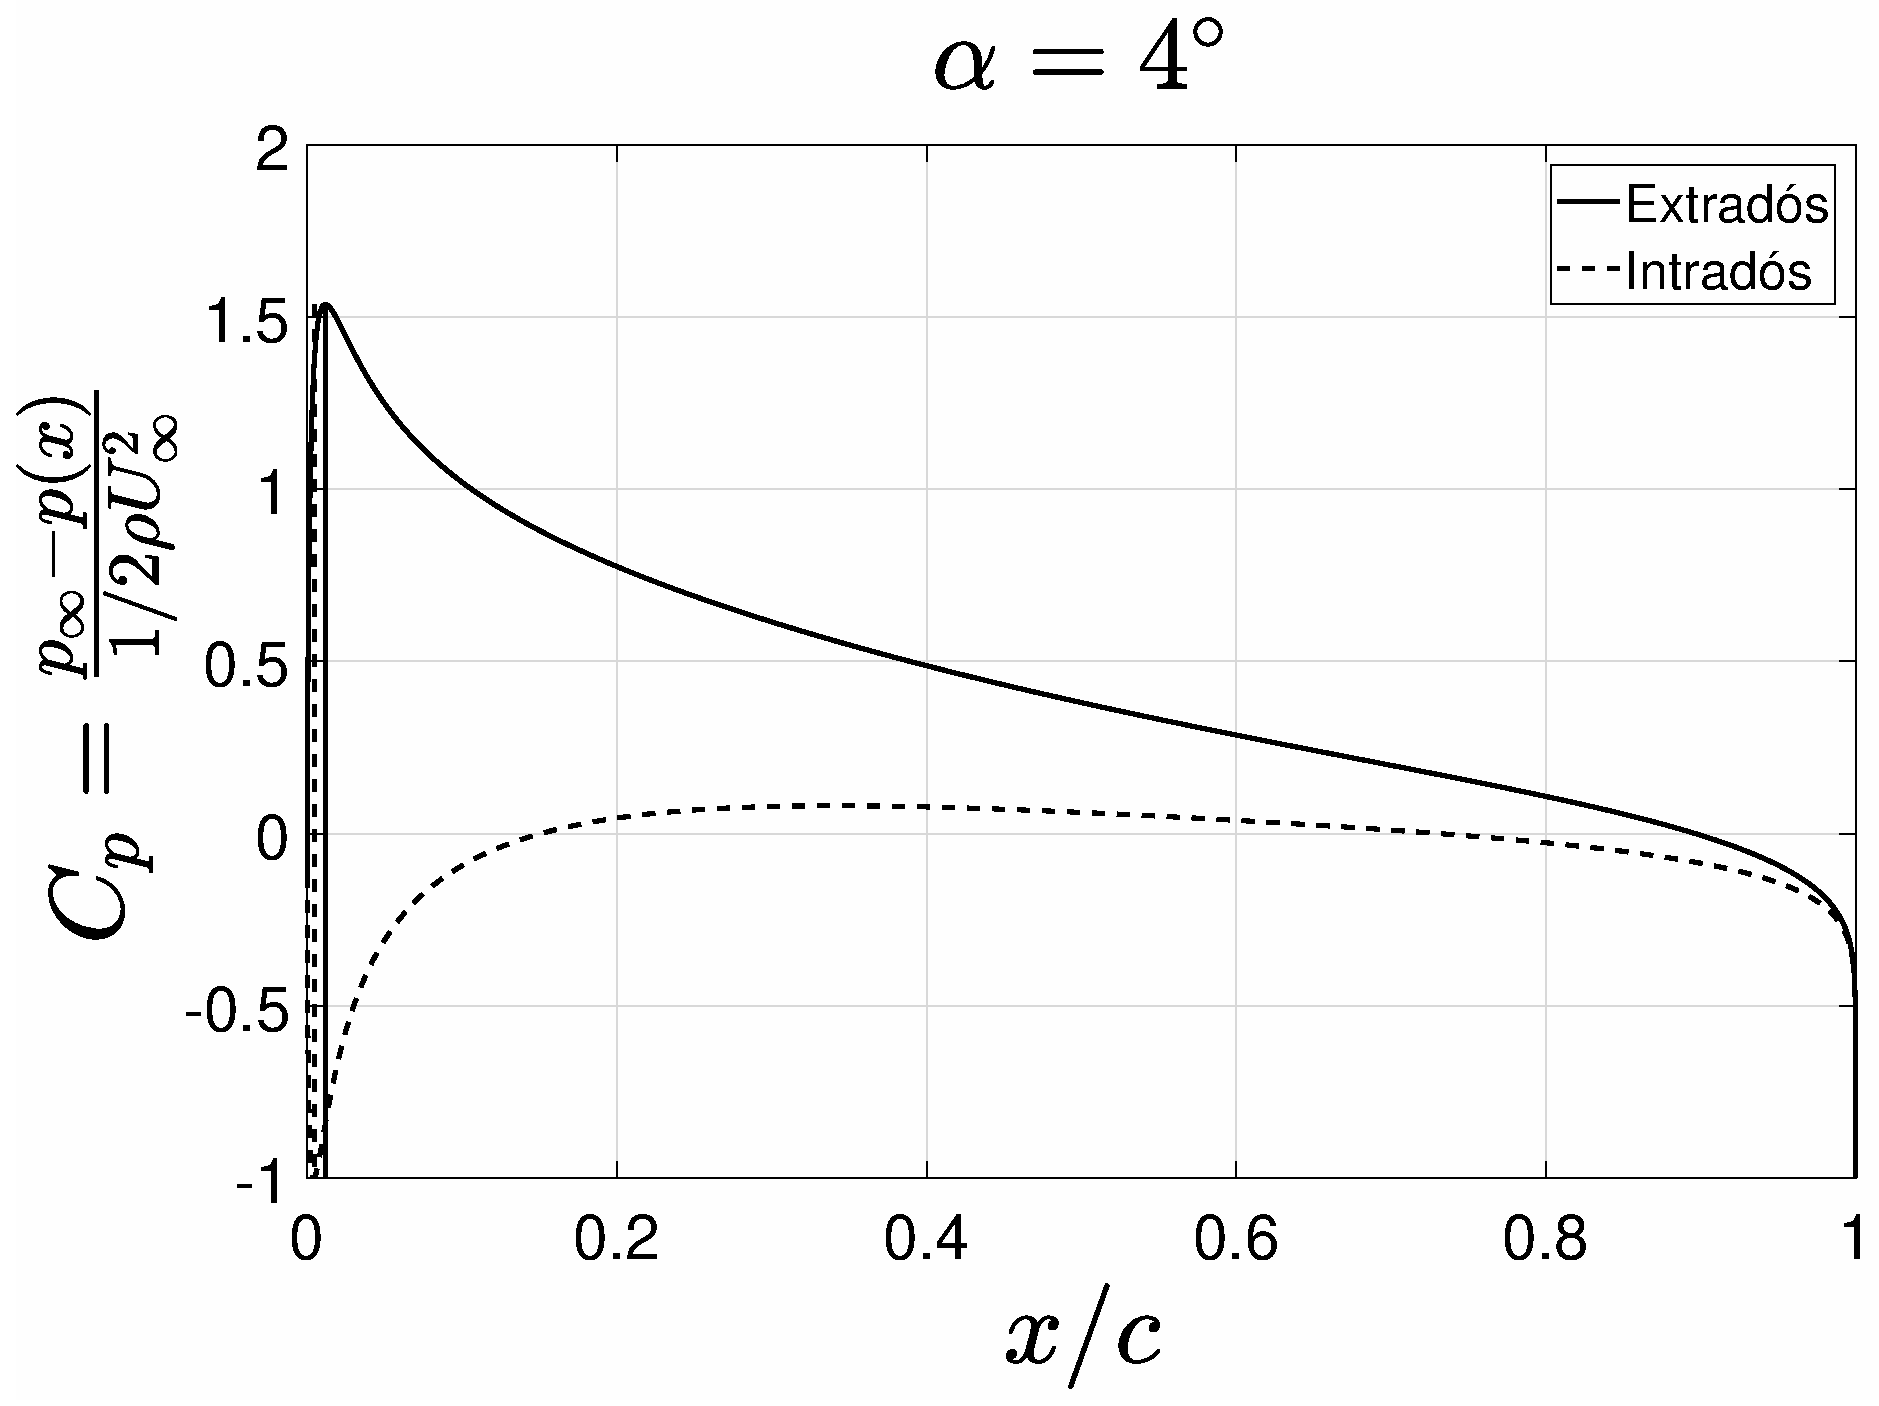
\includegraphics[width = .45\textwidth]{cp.eps}\LABFIG{cp}}
\subfloat[Zoom de $-C_{p}$ en el borde de ataque]{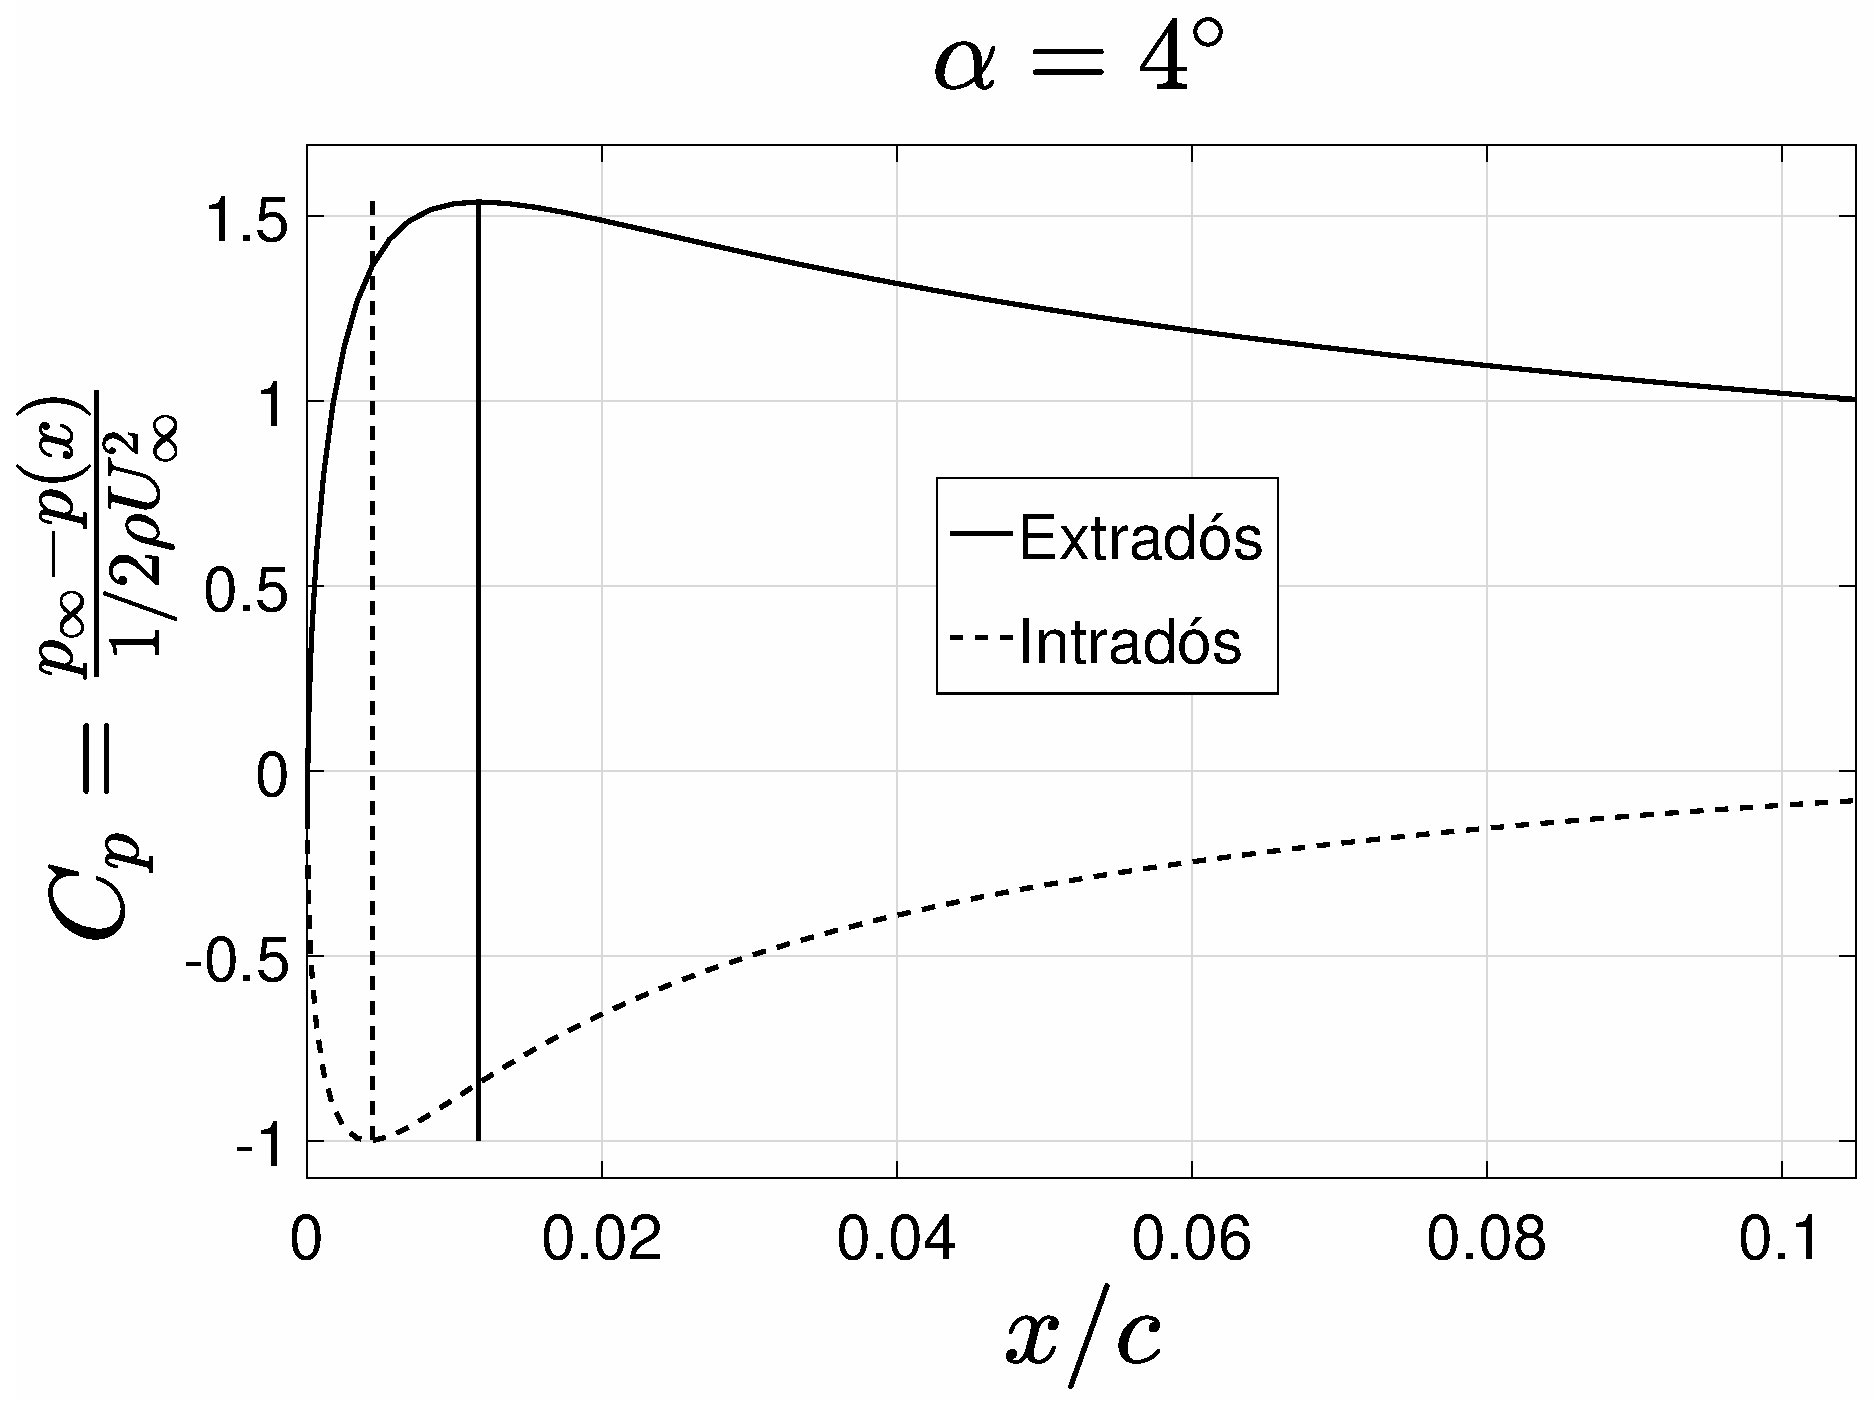
\includegraphics[width=.45\textwidth]{cpZoom.eps}\LABFIG{cpZoom}}
\caption{Resultados de una simulación por el método de elementos de contorno de un perfil simétrico NACA~0012 cuando sobre él incide una corriente con ángulo de ataque $\alpha = 4^{\circ}$. En la \FIG{upotencial} se representa el campo de velocidad longitudinal de perturbación y en la \FIG{cp} su correspondiente campo de presión. La \FIG{upotencialZoom} y la \FIG{cpZoom} se muestra ampliada la zona cercana al borde de ataque, donde existen como puede apreciarse fuertes gradientes favorables de presión.}
\LABFIG{resultadoPotencial}
\end{figure}

% !TEX root =../LibroTipoETSI.tex
\chapter{Ejemplo de Capítulo}\LABCHAP{CAPEJ}
\pagestyle{esitscCD}
\epigraph{ Una de las virtudes del ingeniero es la eficiencia.  }{Guang Tse}

%\lettrine[lraise=0.7, lines=1, loversize=-0.25]{E}{l} 
\lettrine[lraise=-0.1, lines=2, loversize=0.25]{E}l \emph{formato de capítulo }\index{formato!de capítulo} abarca diversos factores. Un capítulo puede incluir, además de texto, los siguientes elementos:
%http://en.wikibooks.org/wiki/LaTeX/List_Structures#Customizing_Lists

\begin{itemize}\itemsep1pt \parskip0pt \parsep0pt
\item \indexit{Figuras}
\item \indexit{Tablas}
\item \indexit{Ecuaciones}
\item \indexit{Ejemplos}
\item \indexit{Resúmenes}, con recuadros en gris, por ejemplo
\item \indexit{Lemas}, \indexit{corolarios}, \indexit{teoremas},... y sus demostraciones
\item \indexit{Cuestiones}
\item \indexit{Problemas} propuestos
\item ...
\end{itemize}

En este capítulo se propone incluir ejemplos de todos estos elementos, para que el usuario pueda modificarlos fácilmente para su uso. Consulte el código suministrado, para ver cómo se escriben en \LaTeX.

\section{Ejemplo de sección}\LABSEC{SEC}
%
En la \FIG{FIG} se incluye a modo de ejemplo la imagen del logo de la \gls{ETSI} \footnote{Se usa aquí el package de acrónimos, que la primera vez define el acrónimo y ya luego sólo incluye el mismo. Esto facilita luego generar de forma automática la lista de acrónimos.}. El código para que aparezca dicha imagen se muestra en el cuadro siguiente:



Si nos detenemos en los comandos que hemos utilizado, con \ttcolor{width} se controla el ancho, y se escala así el tamaño de la imagen. En \LaTeX existen diversas opciones para situar la figura en la página: con \ttcolor{t} o \ttcolor{b} se le indica que las incluya arriba o abajo (top/bottom) y con \ttcolor{!} se le pide que la deje dónde está, tras el texto anterior.


\begin{lstlisting}[language=TeX,caption={Código para incluir una figura}, breaklines=true, label=prg01-01]
\begin{figure}[htbp]
\centering

\includegraphics[width=3 cm]{capituloLibroETSI/figuras/logoESI.pdf}
\caption{Logo de la ETSI}
\label{fig:figura1}
\end{figure}
\end{lstlisting}


\begin{figure}[htbp]
\centering
%
\includegraphics[width=0.2\linewidth]{capituloLibroETSI/figuras/logoESI.pdf}

\includegraphics[width=3 cm]{CapituloLibroETSI/figuras/logoESI.pdf}
\caption{Logo de la ETSI}
\LABFIG{FIG} %Esto es una forma propia de los autores de gestionar las etiquetas y referencias
\end{figure}
%

Para dar énfasis a algún texto, usamos \ttcolorc{emph}. %Este comando es de los denominados \emph{inteligentes} apareciendo el texto \emph{resaltado} dependiendo del contexto.  
Así, por ejemplo, 
\begin{caja}
\emph{No olvide intentar utilizar este formato en sus publicaciones de la \gls{ETSI}}
\end{caja}
hace aparecer el anterior texto en itálica. Pero si escribiésemos, por ejemplo, 
\begin{caja}
\emph{No olvide intentar utilizar este formato \emph{siempre} en sus publicaciones de la \gls{ETSI}}
\end{caja}
vemos cómo hemos destacado la palabra ``siempre'' en torno a su contexto. Para ello, hemos escrito, realmente, \comandos{emph}{siempre} dentro de la frase original.
%
\subsection{Ejemplo de subsección}\LABSSEC{EjSS}
%
Si se usaba \ttcolorc{section} para indicar una sección, se utiliza \ttcolorc{subsection} para una subsección.


\section{Elementos del texto}
%

\subsection{Figuras}

Además del tipo de figura que vimos anteriormente, el normal, podemos desear incluir una figura en modo apaisado ocupando toda la página. Para ello utilizamos el entorno de figura siguiente \comandos{begin}{sidewaysfigure}, cuyo resultado se puede observar en la \FIG{FigApaisada}. 

\begin{sidewaysfigure}
\centering
%
\includegraphics[width=0.2\linewidth]{capituloLibroETSI/figuras/logoESI.pdf}

\includegraphics[width=3 cm]{CapituloLibroETSI/figuras/logoESI.pdf}
\caption{Logo de la ETSI}
\LABFIG{FigApaisada}
\end{sidewaysfigure}

Aunque puede optar por la forma que desee, en el fichero \ttcolor{notacion.sty} se incluyen definiciones para que pueda usar \comandos{LABFIG}{etiqueta} y \comandos{FIG}{etiqueta} para poner una etiqueta y hacer referencia a la misma luego. Además, está definido para que \comandos{FIG}{etiqueta} incluya por delante el término Figura.

\subsection{Tablas}
A modo de ejemplo, \TAB{Tab1} incluye un ejemplo de tabla. Al igual que con figura, si usa \ttcolor{notacion.sty} puede usar \comandos{LABTAB}{etiqueta} y \comandos{TAB}{etiqueta} para poner una etiqueta y una referencia, y el \comandos{TAB}{etiqueta} ya incluye el nombre Tabla por delante.

Una alternativa al uso de estos comandos está representado por el uso del comando \ttcolorc{autoref\{etiqueta\}} que, en conjunción con el paquete \ttcolor{babel} genera automáticamente los nombres de Figura o Tabla, en función de la etiqueta correspondiente.

\begin{table}[h]
%\small
\caption{Valores de parámetros}
\begin{center}
\begin{tabular}{p{7cm}p{2cm}p{2cm}} %Con esto definimos el ancho de cada columna
Definición & notación & valor\\
 \hline
Potencia transmitida	(entregada a antena) & $P_{et}$ & -5 a 20 dBm	\\
Ganancia antenas & $G$ & $40.5$ dBi\\	
 \hline
\end{tabular}
\end{center}
\LABTAB{Tab1}
\end{table}%

\subsection{Listados de programas}
Es muy habitual en nuestros documentos que tengamos que incluir listados de programas. Para ello, se propone la utilización de un paquete denominado \ttcolor{listings}. Se obtiene con él un listado como el mostrado en el \autoref{prg02-01} de \matlab siguiente: 

\begin{lstlisting}[language=Matlab,caption={Representación de la función $\rect(t-T/2)$}, breaklines=true, label=prg02-01]
clear all
close all
T = 1;
A = 1;
L = 100;
tstep = T/L;                                
t = 0:tstep:T-tstep;   
g_t = A*ones(1,L); 
figure(1);
subplot(211);
h=plot(t,g_t); axis( [0 T -A-0.1 A+0.1]);
set(h,'linewidth', 1.0);
ylabel('g(t)'), xlabel('t[s]'); grid on;

g_n = g_t;
subplot(212);
h=stem(g_n, '.', 'filled'); axis( [1 L -0.1 A+0.1]);
set(h,'linewidth', 1.0);
ylabel('g(n)'), xlabel('n');
\end{lstlisting}

También se puede generar en este caso una relación de los códigos usados en nuestro documento, de manera equivalente a la relación de figuras o tablas. Para ello, observar la correspondiente codificación en el fichero principal.
 
\subsection{Ecuaciones}%%%%%%%%%%%%%%%%%%%%%%%%%%%%%%%%%%%%%%%
Para escribir expresiones matemáticas, como por ejemplo $2+2=4$, sólo hace falta que meta la expresión entre símbolos \ttcolor{\$}. En el fichero notacion.sty se incluyen muchas definiciones para facilitar la escritura de estas expresiones y de ecuaciones. Para escribir una ecuación, con una o más líneas, se aconseja utilizar \ttcolor{align}, como en el siguiente ejemplo, en las ecuaciones \EQ{Eq1}-\EQ{Eq3},
\begin{align}
 T     &=kT_b  \LABEQ{Eq1}, \\
 R_b&=\frac{1}{T_b }	, \\
 D    &=\frac{1}{T}=\frac{R_b }{k}=\frac{R_b}{\log_2 M}. \LABEQ{Eq3}
\end{align}
Si no quiere numerar una línea, utilice las instrucción \comando{nonumber} antes de poner \verb+\\+  para escribir la siguiente línea. Y con \& puede alinear las ecuaciones. 

Un ejemplo más complejo de ecuaciones sería el siguiente: decimos que el vector aleatorio $\vc{Z}$ es gaussiano si su función densidad de probabilidad conjunta viene dada por:
\begin{equation}\label{eq02-x131}
f_{\vc{Z}}\left( {\vc{z}} \right)= \frac{1}{\left( {2\pi} \right)^{N}{\left| {\vc{C_{Z}}} \right|}^{1/2}}\e^{-\frac{1}{2}\left( {\vc{z}-\vc{m_{Z}}} \right)\trs\vc{C_{Z}}^{-1}\left( {\vc{z}-\vc{m_{Z}}} \right) }
\end{equation}
con el vector media la matriz $\vc{m_{Z}}$ y la matriz de covarianza real $\vc{C_{Z}}$ $\left( {2N \times 2N} \right)$ simétrica definida positiva dado por:
\begin{equation}\label{eq02-x132}
\vc{m_{Z}}=\begin{bmatrix}
\vc{m_{X}}\\
\vc{m_{Y}}
\end{bmatrix}, \quad
\vc{C_{Z}}=\begin{bmatrix}
\vc{C_{X\hphantom{X}}} & \vc{C}_\vc{XY}\\
\vc{C_{YX}} & \vc{C_{Y\hphantom{X}}}
\end{bmatrix}
\end{equation}

con el vector $\bm{\omega}$ dado por:
\begin{equation}\label{eq02-y410}
\bm{\omega}=\begin{bmatrix}
\omega_{1}\\
\vdots \\
\omega_{N}\\
\omega_{N+1}\\
\vdots \\
\omega_{2N}
\end{bmatrix}
\end{equation}
Si no desea que se numere una ecuación puede poner asterisco, tanto en el entorno \verb+equation+ como \verb+align+.


\subsection{Ejemplos}%%%%%%%%%%%%%%%%%%%%%%%%%%%%%%%%%%%%%%%

Para incluir un ejemplo, utilize el entorno \comando{ejmp}, usando el entorno \comando{begin\{ejmp\}} y \comando{end\{ejmp\}}, y para la solución el entorno  \comando{begin\{sol\}}. 

\begin{ejmp}
Calcule $2+2$.
\end{ejmp}
\begin{sol}
%
Para resolver esto se puede utilizar que $1+1=2$, de la siguiente forma
\begin{equation*}% con el * se evita que se numere la ecuación
2+2=(1+1)+(1+1)=4,
\end{equation*}
donde se ha contado, pruebe a utilizar los dedos de su mano, a cuatro.
\end{sol}

Observad que antes de comenzar el ejemplo y tras su finalización se han incluido unos \emph{filetes} a modo de resalte en el texto. En el caso de una serie de ejemplos, los entornos \comando{begin\{ejmpn\}} y  \comando{begin\{soln\}}, junto con los entornos de cierre correspondientes, permiten que no existan estos filetes entre los ejemplos y soluciones intermedias de la serie.
 
\subsection{Lemas, teoremas y similares}

Se incluyen ejemplos de estos elementos de texto. Empezamos con la \DFN{D11} y la \PRP{P11}:

\begin{defn}[Suma]\LABDFN{D11}
 La suma es la operación que permite contar sobre un número, otro.
\end{defn}


\begin{prop}[Suma]\LABPRP{P11}
 Los números enteros se pueden sumar.
\end{prop}


\begin{lema}[Suma de 1 y 1]\LABLEM{L11}
 La suma $1+1$ es igual a $2$.
\end{lema}
\begin{proof}
Ponga un dedo a la vista, junto a otro, y cuéntelos.
\end{proof}


\begin{teor}[Suma]\LABTHM{T11}
 La suma de cualquier número y dos es igual a la suma del mismo número más uno más uno.
\end{teor}
\begin{proof}
Por inducción y el \LEM{L11}.
\end{proof}

\begin{coro}[Contables]\LABCOR{C11}
  Los números enteros son contables.
\end{coro}
\begin{proof}
Por el \THM{T11}.
\end{proof}


\subsection{Resúmenes}%%%%%%%%%%%%%%%%%%%%%%%%%%%%%%%%%%%%%%%
Para incluir un resumen de una sección o un conjunto de secciones o en cualquier otro punto que consideremos interesante, se utiliza el entorno \comando{begin\{Resumen\}}, que admite como parámetro opcional un nombre que queramos asignarle al resumen. Por defecto, se denomina ``Resumen''. Observar que se ha modificado la cabecera de las páginas impares. Una vez finalizado el resumen, con el comando \comando{end\{Resumen\}}, se recupera la anterior cabecera automáticamente. Los resúmenes que se deseen incluir aparecen en la tabla de contenidos como una sección sin numeración, con el nombre elegido o el nombre por defecto de Resumen. En el siguiente ejemplo hemos utilizado este parámetro opcional de nombre.

\begin{Resumen}[Resumen de Teoría de Información]
\noindent Debido al considerable número de definiciones, teoremas y propiedades que hemos descrito en los apartados anteriores, vamos a presentar un resumen de los principales resultados, no necesariamente en el mismo orden que el expuesto anteriormente. Supondremos en este resumen que las variables aleatorias $X$,  $Y$ y $Z$ son discretas, definidas en el alfabeto $\calg{X}$, $\calg{Y}$  y  $\calg{Z}$ respectivamente. 

\subsubsection*{Entropía de una variable aleatoria discreta}
Se define la entropía $H\left( {X} \right)$ de una variable aleatoria discreta $X$ , con función masa de probabilidad $p\left( {x} \right)$, en la forma:
\begin{equation*}
H\left( {X} \right)= -\sum_{x\in \calg{X} }{p\left( {x} \right)\log p\left( {x} \right)}=\E\left[ -{\log p\left( {X} \right)} \right]
\end{equation*}
\begin{enumerate}
\item Se cumple:
\begin{equation*}
 0\le H\left( {X} \right) \le \log \card{\calg{X}}
\end{equation*}
 con la igualdad en la izquierda si y sólo si $p\xb{i}=1$ para algún $x_{i} \in \calg{X}$ y con la igualdad a la derecha si y sólo si la variable aleatoria está uniformemente distribuida; esto es, $p\xb{i}=1/\card{\calg{X}} \; \mbox{para todo }i$.
 \item $H\left( {X} \right)=0$ si y sólo si $X$ es determinista.
\item $H\left( {X} \right)=H\left( {p\left( {x} \right)} \right)$ es una función cóncava en $p\left( {x} \right)$.
\item Se define la \emph{Función de Entropía Binaria} en la forma:
\begin{equation*}
h_{b}\left( {p} \right) \eqdef -p\log p-\left( {1-p} \right)\log\left( {1-p} \right)\end{equation*}
\item La función entropía binaria $h_{b}\left( {p} \right)$ es una función cóncava en $p$.
\item Si $X$ y $\hat X$ son dos variables aleatorias estadísticamente independientes igualmente distribuidas, 
\begin{equation*}
\Pr\left( {X=\hat X} \right) \ge 2^{-H\left( {X} \right)}
\end{equation*}
con la igualdad si y sólo si $X$ tiene una distribución uniforme.
\end{enumerate}

\subsubsection*{Entropía conjunta y entropía condicional}
Definimos la \emph{entropía conjunta} de las variables aleatorias $X$ e $Y$, $H\left( {X,Y} \right)$ en la forma:
\begin{equation*}
H\left( {X,Y} \right)=\sum_{x\in \calg{X} }{\sum_{y\in \calg{Y}}{p\left( {x,y} \right)\log \frac{1}{p\left( {x,y} \right)}}}=\E\left[ {-\log p\left( {X,Y} \right)} \right]
\end{equation*}

Definimos la \emph{entropía condicional} $H\left( {X \mid Y} \right)$ en la forma:
\begin{align*}
H\left( {X \mid Y} \right)&=\sum_{y\in \calg{Y}}{p\left( {y} \right)H\left( {X \mid Y= y} \right)}=  \\
&=-\sum_{x\in \calg{X}}{\sum_{y\in \calg{Y}}{p\left( {x,y} \right) \log p\left( {x \mid  y} \right)}}= \\
&=\E\left[ {-\log p\left( {X\mid Y} \right)} \right]
\end{align*}

\begin{enumerate}
\itemv[10]
\begin{equation*}
H\left( {X,Y} \right) \le H\left( {X} \right)+ H\left( {Y} \right)
\end{equation*}
con la igualdad si y sólo si $X$ e $Y$ son estadísticamente independientes.
\itemv[10]
\begin{align*}
H\left( {X\mid Y} \right) &\le H\left( {X} \right) \\
H\left( {Y\mid X} \right) &\le H\left( {Y} \right)
\end{align*}
con la igualdad si y sólo si $X$ e $Y$ son estadísticamente independientes.
\item $H\left( {X\mid Y} \right)=0$ si y sólo si $X$ es una función de $Y$.
\itemv[10]
\begin{equation*}
H\left( {X \mid X} \right) =0
\end{equation*}
\itemv[10] 
\begin{equation*}
H\left( {X,Y} \right)=H\left( {Y} \right)+H\left( {X\mid Y} \right)
\end{equation*}
\itemv[10] 
\begin{equation*}
H\left( {X,Y} \right)=H\left( {X} \right)+H\left( {Y\mid X} \right)
\end{equation*}
\itemv[10] 
\begin{equation*}
H\left( {X,Y \mid Z} \right)=H\left( {X\mid Z} \right)+H\left( {Y\mid X,Z} \right)
\end{equation*}
\item \emph{Desigualdad de Fano} Sean $X$ y $\hat{X}$ dos variables aleatorias que toman valores en el mismo alfabeto \calg{X}. Se verifica:
\begin{equation*}
H\left( {X\mid \hat{X}} \right) \le h_{b}\left( {p\xb{e}} \right)+p\xb{e}\log \left( {\card{\calg{X}}-1} \right)
\end{equation*}
\end{enumerate}
%
\subsubsection*{Reglas de las cadenas}
Sea $\mathbf{X}$   un vector formado por las $N$ variables aleatorias $X_{i}, i=1, 2, \ldots,N$.
\begin{enumerate}
\item \emph{Regla de la cadena para la entropía}
\begin{align*}
H\left( {X_{1}, X_{2}, \ldots, X_{N}} \right)&=\sum_{i=1}^{N}{H\left( {X_{i}\mid X_{1},\ldots, X_{i-1}} \right)}= \\
&=H\left( {X_{1}} \right)+H\left( {X_{2}\mid X_{1}} \right)+ \cdots +H\left( {X_{N}\mid X_{1},\ldots, X_{N-1}} \right) 
\end{align*}
\item \emph{Regla de la cadena para la entropía condicional}
\begin{equation*}
H\left( {X_{1}, X_{2}, \ldots, X_{N} \mid Y} \right)=\sum_{i=1}^{N}{H\left( {X_{i}\mid X_{1},\ldots ,X_{i-1}, Y} \right)}
\end{equation*}
\item \emph{Regla de la cadena para la información mutua}
\begin{equation*}
I\left( {X_{1}, X_{2}, \ldots, X_{N} ; Y} \right)=\sum_{i=1}^{N}{I\left( {X_{i} ;Y \mid X_{1},\ldots, X_{i-1}} \right)}
\end{equation*}
\item \emph{Regla de la cadena para la Información Mutua Condicional}
\begin{equation*}
I\left( {X_{1}, X_{2}, \ldots, X_{N} ; Z \mid Y} \right)=\sum_{i=1}^{N}{I\left( {X_{i} ;Z \mid X_{1},\ldots, X_{i-1},Y} \right)}
\end{equation*}
\end{enumerate}
\end{Resumen}

\section{Una nueva sección después del resumen}


%%%%%%%%%%%%%%%%%%%%%%%%%%%
%%%%%%%%%%														
%%%%%%%%%%					Problemas							
%%%%%%%%%%														
%%%%%%%%%%%%%%%%%%%%%%%%%%%


\cleardoublepage
\subchapter{Problemas Propuestos}
\setenumerate[1]{label=\bfseries{\alph*)\quad}, labelindent=\parindent}
\setenumerate[2]{label=\bfseries\arabic*.}
\setenumerate[3]{label=\bfseries{\roman*})}
\pagestyle{probprop}
\captionsetup[figure]{textformat=simple}

\noindent Esto es un ejemplo de cómo incluir cuestiones y/o problemas al final de un capítulo, con o sin solución. Para poner un problema o cuestión, usar  \comando{begin\{prob\}} y \comando{end\{prob\}}. Para incluir la solución, a continuación usar \comando{begin\{soln\}} seguido del texto terminado en \comando{end\{soln\}}.

% P02-01
\begin{prob}
Sean $A$, $B$ y $C$ sucesos de un cierto experimento con probabilidades dadas por:
\begin{align*}
\Pr\left( {A} \right)=&\frac{1}{3}\\
\Pr\left( {B} \right)=&\frac{1}{4}\\
\Pr\left( {C} \right)=&\frac{1}{5}\\
\Pr\left( {A\cap B} \right)=&\frac{1}{12}\\
\Pr\left( {A\cap C} \right)=&\frac{1}{15}\\
\Pr\left( {B\cap C} \right)=&\frac{1}{20}\\
\Pr\left( {A\cap B\cap C} \right)=&\frac{1}{30}
\end{align*}
\begin{enumerate}
\item ¿Son los sucesos independientes dos a dos? ¿Son estadísticamente independientes?
\item Encontrar $\Pr\left( {A\cup B} \right)$.
\item Encontrar $\Pr\left( {A\cup B\cup C} \right)$.
\end{enumerate}
\end{prob}

\begin{prob}
Suponer que tenemos una moneda con las siguientes características: cuando se lanza, la probabilidad de que salga cara es  $\Pr\left( {c} \right)=p$ y la probabilidad de que salga cruz $\Pr\left( {+} \right)=q$. Lanzamos dos veces la moneda y queremos conocer acerca de la independencia estadísticade los siguientes sucesos:
\begin{align*}
A& = \textrm{Sale c en la primera tirada}\\
B& = \textrm{En las dos tiradas sale lo mismo}\\
C& = \textrm{Sale c en la segunda tirada}
\end{align*}
\end{prob}

\begin{prob}
Determinar la media, la autocorrelación y el espectro densidad de potencia de la salida de un sistema con respuesta impulsiva dada por:
\begin{equation*}
h(n) = \begin{cases}
1 &n=0,2 \\
-2 &n=1  \\
0 & \text{en cualquier otro caso} \\
\end{cases}
\end{equation*}
cuando la señal de entrada es un ruido blanco $X(n)$ con varianza 
$\sigma_X^2$.
\end{prob}

\begin{soln}
Si el ruido es blanco, su valor esperado será cero y su espectro densidad de potencia será una constante: $S_{X}\left( {\Omega} \right)=C$. Calculemos su autocorrelación. Se tiene:
\begin{align*}
 R_X (k)&=\L[F]\ ^{-1}\left[ {S_X \left( \Omega \right)} 
\right]=\L[F]\ ^{-1}\left[ C \right]=\frac{1}{2\pi }\int_{-\pi }^\pi 
{Ce^{jk\Omega }\mathrm{d}\Omega } =
\begin{cases}
   {k\ne 0}	   &  \frac{C}{2\pi }\left. {\frac{\e^{jk\Omega }}{jk}} \right|_{-\pi }^\pi\\
     k=0 & C \\
\end{cases}
\;\Rightarrow \\ 
 R_X (k)&=C\delta(k)=
 \begin{cases}
      C & k= 0\\
      0 & k \ne 0
\end{cases}
 \end{align*}

Ahora bien:  (...)
\end{soln}



%%%%%%%%%%%%%%%%%%%%%%%%%%%%%%%%%%%%%%%
%:Material suplementario

%%%%%%%%%%%%%%%%%%%%%%%%%%%%%%%%%%%%%%%

%%%%%%%%%%%%%%%%%%%%%%%%%%%%%%%%%%%%%%%
\subchapter{Anexo}
\pagestyle{esitscCD}
%

\epigraph{Si quiere introducir un separador dentro de un capítulo puede utilizar la instrucción subchapter. Esto le puede interesar, por ejemplo, para introducir alguna información adicional al final de un capítulo como un anexo al mismo.}


%\noindent 
\lettrine[lraise=-0.1, lines=2, loversize=0.25]{E}{n} las secciones que siguen vamos a repasar algunas materias que utilizamos ampliamente a lo largo del texto y que sostienen de forma rigurosa el estudio de las comunicaciones digitales.

\section{Señales: definición y clasificación}
%
Una \index{señal} puede definirse como una función que transmite información generalmente sobre el estado o el comportamiento de un sistema físico, \cite{oppenheim}. Aunque las señales puedan representarse de muchas maneras, en todos los casos la información está contenida en la variación de alguna magnitud física. Matemáticamente se representan como una función de una  o más variables independientes. Por ejemplo, una señal de voz se puede representar como una función del tiempo y una imagen fotográfica puede representarse como una variación de la luminosidad respecto a dos parámetros espaciales. En cualquier caso, es una práctica común denotar como tiempo, $t$, a la variable independiente, en el caso de una variación continua de la variable independiente, y $n$ en caso contrario.
%
\subsection{Clasificación de señales}%
Establezcamos a continuación una clasificación de las señales atendiendo a diversos puntos de vista.
%
\subsubsection*{Señales deterministas y aleatorias}
%
\index{señal!determinista}\index{señal!aleatoria} %% Índice
Una señal se clasifica como determinista cuando no hay incertidumbre alguna acerca del valor que tiene en cualquier instante de tiempo. Estas señales pueden modelarse como una función matemática, por ejemplo, $g\left( {t} \right) = 10 \cos\left( {4\pi t^{2}} \right)$. 

Una señal aleatoria es aquella para la que existe cierta incertidumbre respecto a su valor. Matemáticamente vamos a modelarla como una función muestra de un proceso aleatorio.

Para que una señal transmita información debe tener un carácter aleatorio, \cite{wiener}. 
%
\subsubsection*{Señales periódicas y no periódicas.}
%
\index{señal!periódica}\index{señal!no periódica}
Una señal $g(t)$ es periódica, con periodo $T_{0}$, si existe una cantidad $T_{0} >$0 tal que:
\begin{equation}
\label{eq01ms-1}
g(t)=g(t+T_0 )\quad \forall t
\end{equation}
siendo $T_{0}$ el valor más pequeño que cumple esta relación. Una señal que no cumpla \eqref{eq01ms-1} se denomina no periódica.
%
\subsubsection*{Señales analógicas, discretas, muestreadas y digitales}
%
\index{señal!analógica}\index{señal!discreta}\index{señal!muestreada}\index{señal!digital}			%% Índice
Una señal analógica $g(t)$ es aquella que está definida para todo $t$. Una señal discreta sólo está definida en un conjunto numerable\footnote{\label{foot02-01}Un conjunto  es numerable o contable cuando sus elementos pueden ponerse en correspondencia uno a uno con el conjunto de los números naturales. Con posterioridad veremos que el concepto de conjunto numerable o contable juega un papel importante en el desarrollo de numerosos aspectos de la teoría.} de valores del tiempo. Una señal muestreada está definida para todo instante de tiempo, aunque sólo puede tomar valores en un conjunto numerable y una señal digital es aquella que sólo está definida en un conjunto numerable de valores del tiempo y toma valores en un conjunto numerable.
%



%%%%%%%%%%%FIN


\captionsetup[figure]{textformat=period}
\endinput

 

% !TEX root =../LibroTipoETSI.tex
\chapter{Ejemplo de Capítulo de Problemas}\LABCHAP{CAPPB}

\epigraph{Este es un ejemplo de capítulo de libro de problemas, donde cada sección es un problema distinto, con 
enunciado y solución. Se incluye un problema cualquiera, para que el lector pueda aprender cómo utilizarlo. El enunciado de cada problema comienza con \comando{problema} cómo si se tratara de una sección más. Como tal aparecerá en el índice del libro y en las cabeceras de páginas correspondientes.} 

\lettrine[lraise=-0.1, lines=2, loversize=0.25]{B}{la} bla,..., los conceptos más relevantes necesarios para la resolución de los problemas de este capítulo se refiere al lector al texto \cite{Hernando08}. La notación es la incluida al comienzo de este documento.
%
%incluyeron en los Apartados \SSEC{Ruido}, \SSEC{Sensibilidad}, y \SSEC{Nolinealidad}. 
Los conceptos necesarios para resolver los problemas planteados se pueden consultar en \cite{Murillo07}, excepto los relacionados con el cálculo de propagación, para los que se puede recurrir a \cite{Hernando08}. A continuación se incluye una descripción de los cálculos más relevantes utilizados en estos problemas, utilizando la notación introducida al comienzo del texto.


\section{Ruido y sensibilidad}\LABSEC{Ruido}
Vamos a estudiar el ruido y la sensibilidad en ...

\subsection{Temperatura y figura de ruido} \LABSSEC{Ruido}
En este texto, ver comienzo del mismo, se denota por $f_r$ y $T_r$ la figura y la temperatura equivalente de ruido, respectivamente, del receptor, formado éste por los elementos que van desde el conector de antena a la entrada al demodulador. Por otro lado, $f_a$ y $T_a$ se utilizan para denotar la figura y la temperatura equivalente de ruido de la antena. Y $f_s$ y $T_s$ denotan la figura de ruido y la temperatura equivalente del sistema completo, antena más receptor.  Aquí las figuras de ruido están en unidades naturales, y las denotamos por ello en minúsculas. La misma notación para las figuras de ruido en mayúsculas se utilizará para denotar dB. (...)%Por otra parte, se asume adaptación de impedancias en el sistema. 


\subsection{Sensibilidad}\LABSSEC{Sensibilidad}


En radiocomunicaciones digitales es habitual utilizar \cite{Hernando08}
\begin{align}
    \frac{c}{n}=\frac{e_b/T_b}{n_0\cdot B}=\frac{e_b\cdot R_b}{n_0\cdot B},
\end{align}
donde $c$ es la potencia de portadora en u.n., $B$ es el ancho de banda equivalente de ruido y
%\begin{align}
%    w&=\frac{c}{n}\cdot \frac{B}{R_b},
%\end{align}
%donde
$R_b=1/T_b$ es el régimen binario. 
%En comunicaciones digitales, si se utiliza el filtro adaptado como filtro receptor, $B=1/T_s$, y $\frac{c}{n}=\log_2M\cdot w$.

Por otro lado se define $w=e_b/n_0$ como (...)

\section{No linealidad}\LABSSEC{Nolinealidad}
Si la sensibilidad nos impone un mínimo a la potencia mínima recibida, el cálculo de la distorsión por no linealidad permite determinar la potencia máxima que el receptor, o transmisor, puede manejar. 
La distorsión por no linealidad de un dispositivo se mide de diferentes formas. Una de las más utilizadas es calcular la relación esperada entre la potencia útil a la salida, $P_o$, y la potencia de intermodulación de tercer orden, $I_3$. Esta relación, una diferencia si se escribe en decibelios, se denota por relación de protección frente a intermodulación de tercer orden, $RP=P_o-I_3$.

Para calcular este valor se (...)


\problema[Radioenlace del servicio fijo a 13 GHz]{Radioenlace del servicio fijo a 13 GHz. Título muy largo que en realidad no cabría en la cabecera}

Una compañía de telefonía móvil desea instalar un radioenlace digital del servicio fijo a $13$ GHz, para unir dos estaciones base a través de un vano de $15$ km de longitud. El enlace tiene un obstáculo agudo de incidencia rasante, esto es, con despejamiento $h=0$ y que introduce unas pérdidas de 6 dB a la par que evita cualquier reflexión en el suelo. 

Se propone utilizar para ello equipos de la serie Flexi-Hopper de Nokia, cuyos datos se incluyen en la \TAB{resfFHop13} para una transmisión dúplex\footnote{ el $2\times$ indica que se utilizan las dos polarizaciones para transmitir.} de $2 \times 2$E1, resultando $4.2$ Mbps en cada sentido modulados en un radiocanal. Tanto el transmisor como el receptor constan de una unidad interior (IU), al pié de la torre, y una unidad exterior (OU) con la etapa de RF junto a la antena, en el extremo superior de las torres, de 15 m. Se sabe, además, que hay una probabilidad $\eta = 25.73$ \% de que exista actividad multitrayecto en el vano para esa zona climática. Además, para esa zona climática se conoce la atenuación, $A_p$, excedida en el $p$\% del tiempo, ver \FIG{resfFHop13}. 

El operador ha fijado como criterios de calidad el \% del tiempo en el que el sistema sufre interrupciones largas y cortas, y como objetivos que las primeras ($>10$s, $BER>10^{-3}$) no superen el $0.036\%$ y las cortas ($\leq10$s, $BER>10^{-3}$) no superen el 0.006\% anual. El departamento de radio tiene que calcular la mínima potencia transmitida para la que el enlace es viable, evitando así interferencias a otros sistemas. 
 
Se pide 
\begin{enumerate}%[labelindent=\parindent,leftmargin=\parindent, label=\normalfont\bfseries  \alph*)] 
\item Calcular el valor de esta potencia. Indique si es necesario mantener en el diseño el HSB (Hot Stand By).
\end{enumerate}   

\begin{table}[h]
%\small
\caption{Datos de las estaciones, con equipos Flexi-Hopper de Nokia}
\begin{center}
\begin{tabular}{p{8.5cm}p{2.5cm}}
 \hline
Potencia transmitida	(entregada a antena) regulable & -5 a 20 dBm	\\
Ganancia antenas & $40.5$ dBi\\	
Modulación & $\pi/4$-DQPSK\\
%Pérdidas en conectores 1 dB	\\
Potencia recibida necesaria para  $BER = 10^{-3}$ y 2E1 ($4.2$Mbps) & $P_{dr}=-89$ dBm\\
Figura de ruido del sistema & 6 dB\\
HSB 1+1, tanto en OU e IU &\\
Tiempo medio entre fallos para OU & $MTBF$=35 años \\
Tiempo medio entre fallos para IU $MTBF$=110 años \\
Tiempo medio en reparar para OU como IU & $MTTR$=20 horas\\
%Altura de antenas sobre el suelo, 15 m\\
Signatura normalizada del receptor	& $k = log_2 M$ \\
 $M$ el número de puntos de la constelación de la modulación & \\
 \hline
\end{tabular}
\end{center}
\LABTAB{resfFHop13}
\end{table}%
\begin{figure}[h]
\centering 
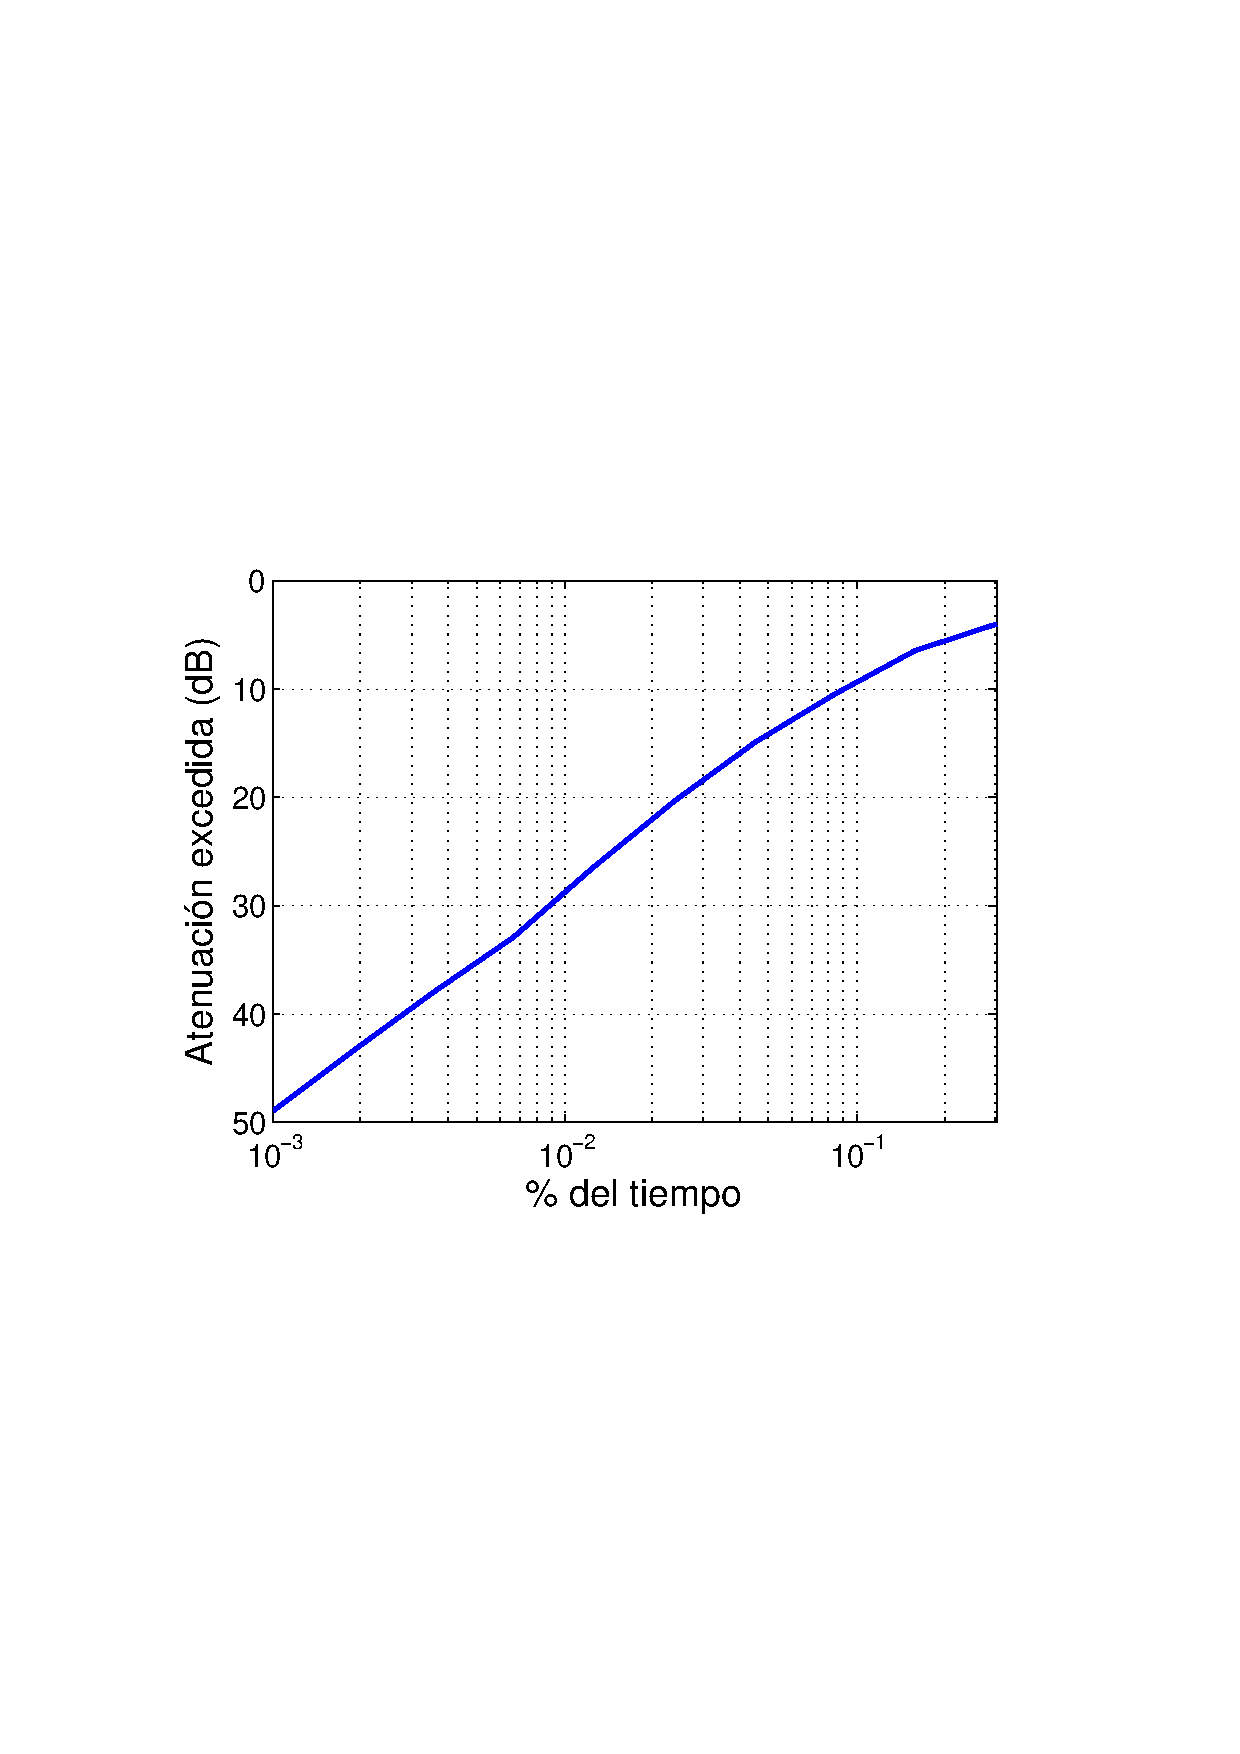
\includegraphics[width=8 cm]{CapituloProblemasLibroETSI/figuras/rain13GHz.pdf}
\caption{Atenuación por lluvia excedida en el $p$ \% del tiempo para 13 GHz y 15 km de distancia}\LABFIG{resfFHop13}%\vspace{-.5 cm}
\end{figure} 

 \begin{solnum}
 \item 
En principio la frecuencia de trabajo no es muy alta, lo que hace pensar que el enlace no estará limitado por lluvia. Los tiempos medios entre fallos son grandes, lo que parece indicar que la indisponibilidad, o interruciones largas, no va a ser un problema. Mientras que sí lo será la pérdida de fidelidad, o interrupciones breves. En todo caso, como el régimen binario es bajo, $\leq 34$ Mbps, el desvanecimiento selectivo no es importante. 

El margen bruto es el que domina en ambos criterios de calidad. De forma que podemos calcular el margen necesario para que se cumplan los objetivos de interrupciones largas (indisponibilidad) y cortas (fidelidad) y quedarnos con el más restrictivo, el mayor.

Calculamos primero el margen necesario para que se cumpla la indisponibilidad. La indisponibilidad de equipos sería la resultante de la suma de la indiponibilidad en cada extremo. En cada extremo tenemos dos equipos funcionando, la IU y la OU, el $MTBF$ equivalente es
\begin{align}
MTBF_e&=(MTBF_{IU}^{-1}+MTFB_{OU}^{-1})^{-1}\nonumber\\
    &=((110\cdot24\cdot 365)^{-1}+(35\cdot24\cdot365)^{-1})^{-1}=2.3259\cdot 10^5.
\end{align}
 Y calculamos
\begin{align}
q&=MTTR/(MTTR+MTBF_e)=20/(20+2.3259\cdot 10^5)=8.5980\cdot 10^{-5}.
\end{align}
 para finalmente estimar la indisponibilidad
\begin{align}
U_{e}&=2 \cdot 100\cdot \binom{M+N}{N+1} (mq)^{N+1}\nonumber\\&=2\cdot 100 \cdot\binom{1+1}{1+1} (1\cdot 8.5980\cdot 10^{-5})^{1+1}
=1.478510^{-6}\%,
\end{align}
%Si no se tuviese HSB, tendríamos 
donde $m=1$ porque tenemos un vano y  $M=N=1$ porque el HSB (Hot Stand By) es $M+N=1+1$. Dado que el máximo valor permitido es $0.036\%$ y que el valor anterior de indisponibilidad por equipos es muy muy pequeño, el máximo valor permitido para indisponibilidad por propagación es, aproximadamente este mismo valor (...)\end{solnum}



%%%%%%%%%%%%
%%%%%%%%%%%%
%%%%%%%%%%%%

\problema{Radioenlace del servicio fijo a 13 GHz}

Una compañía de telefonía móvil desea instalar un radioenlace digital del servicio fijo a $13$ GHz, para unir dos estaciones base a través de un vano de $15$ km de longitud. El enlace tiene un obstáculo agudo de incidencia rasante, esto es, con despejamiento $h=0$ y que introduce unas pérdidas de 6 dB a la par que evita cualquier reflexión en el suelo. 

Se propone utilizar para ello equipos de la serie Flexi-Hopper de Nokia, cuyos datos se incluyen en la \TAB{resfFHop13} para una transmisión dúplex\footnote{ el $2\times$ indica que se utilizan las dos polarizaciones para transmitir.} de $2 \times 2$E1, resultando $4.2$ Mbps en cada sentido modulados en un radiocanal. Tanto el transmisor como el receptor constan de una unidad interior (IU), al pié de la torre, y una unidad exterior (OU) con la etapa de RF junto a la antena, en el extremo superior de las torres, de 15 m. Se sabe, además, que hay una probabilidad $\eta = 25.73$ \% de que exista actividad multitrayecto en el vano para esa zona climática. Además, para esa zona climática se conoce la atenuación, $A_p$, excedida en el $p$\% del tiempo, ver \FIG{resfFHop13}. 

El operador ha fijado como criterios de calidad el \% del tiempo en el que el sistema sufre interrupciones largas y cortas, y como objetivos que las primeras ($>10$s, $BER>10^{-3}$) no superen el $0.036\%$ y las cortas ($\leq10$s, $BER>10^{-3}$) no superen el 0.006\% anual. El departamento de radio tiene que calcular la mínima potencia transmitida para la que el enlace es viable, evitando así interferencias a otros sistemas. 
 
Se pide 
\begin{enumerate}%[labelindent=\parindent,leftmargin=\parindent, label=\normalfont\bfseries  \alph*)] 
\item Calcular el valor de esta potencia. Indique si es necesario mantener en el diseño el HSB (Hot Stand By).
\end{enumerate}   

\begin{table}[h]
%\small
\caption{Datos de las estaciones, con equipos Flexi-Hopper de Nokia}
\begin{center}
\begin{tabular}{p{8.5cm}p{2.5cm}}
 \hline
Potencia transmitida	(entregada a antena) regulable & -5 a 20 dBm	\\
Ganancia antenas & $40.5$ dBi\\	
Modulación & $\pi/4$-DQPSK\\
%Pérdidas en conectores 1 dB	\\
Potencia recibida necesaria para  $BER = 10^{-3}$ y 2E1 ($4.2$Mbps) & $P_{dr}=-89$ dBm\\
Figura de ruido del sistema & 6 dB\\
HSB 1+1, tanto en OU e IU &\\
Tiempo medio entre fallos para OU & $MTBF$=35 años \\
Tiempo medio entre fallos para IU $MTBF$=110 años \\
Tiempo medio en reparar para OU como IU & $MTTR$=20 horas\\
%Altura de antenas sobre el suelo, 15 m\\
Signatura normalizada del receptor	& $k = log_2 M$ \\
 $M$ el número de puntos de la constelación de la modulación & \\
 \hline
\end{tabular}
\end{center}
\LABTAB{resfFHop13}
\end{table}%
\begin{figure}[h]
\centering 
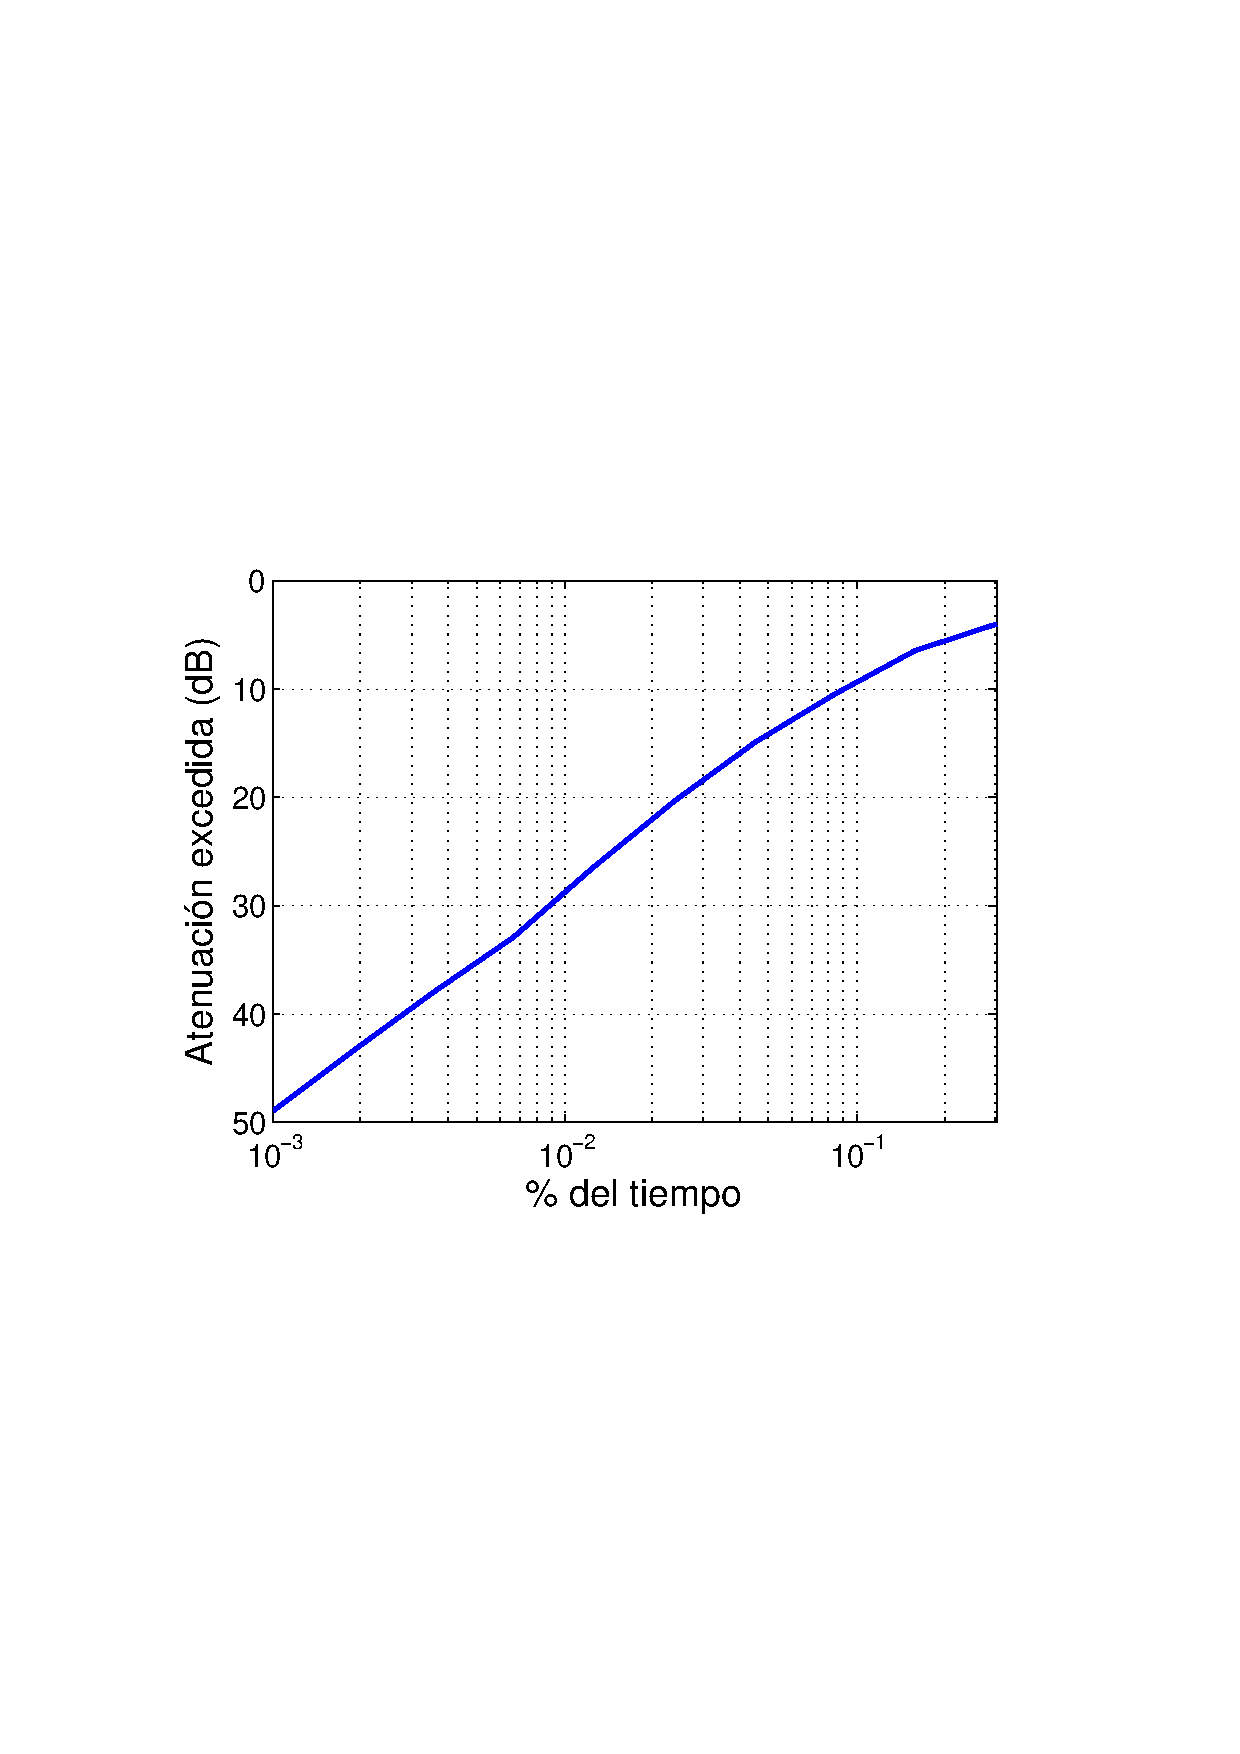
\includegraphics[width=8 cm]{CapituloProblemasLibroETSI/figuras/rain13GHz.pdf}
\caption{Atenuación por lluvia excedida en el $p$ \% del tiempo para 13 GHz y 15 km de distancia}\LABFIG{resfFHop13}%\vspace{-.5 cm}
\end{figure} 

%%%%%%%%%%%
%%%%%%%%%%%
%%%%%%%%%%%

\section{...Ruido y sensibilidad}\LABSEC{Ruido}
Vamos a estudiar el ruido y la sensibilidad en ...

\subsection{...Temperatura y figura de ruido} \LABSSEC{Ruido}
En este texto, ver comienzo del mismo, se denota por $f_r$ y $T_r$ la figura y la temperatura equivalente de ruido, respectivamente, del receptor, formado éste por los elementos que van desde el conector de antena a la entrada al demodulador. Por otro lado, $f_a$ y $T_a$ se utilizan para denotar la figura y la temperatura equivalente de ruido de la antena. Y $f_s$ y $T_s$ denotan la figura de ruido y la temperatura equivalente del sistema completo, antena más receptor.  Aquí las figuras de ruido están en unidades naturales, y las denotamos por ello en minúsculas. La misma notación para las figuras de ruido en mayúsculas se utilizará para denotar dB. (...)%Por otra parte, se asume adaptación de impedancias en el sistema. 

\subsection{...Temperatura y figura de ruido} \LABSSEC{Ruido}
... En este texto, ver comienzo del mismo, se denota por $f_r$ y $T_r$ la figura y la temperatura equivalente de ruido, respectivamente, del receptor, formado éste por los elementos que van desde el conector de antena a la entrada al demodulador. Por otro lado, $f_a$ y $T_a$ se utilizan para denotar la figura y la temperatura equivalente de ruido de la antena. Y $f_s$ y $T_s$ denotan la figura de ruido y la temperatura equivalente del sistema completo, antena más receptor.  Aquí las figuras de ruido están en unidades naturales, y las denotamos por ello en minúsculas. La misma notación para las figuras de ruido en mayúsculas se utilizará para denotar dB. (...)%Por otra parte, se asume adaptación de impedancias en el sistema. 

\subsection{...Temperatura y figura de ruido} \LABSSEC{Ruido}
... En este texto, ver comienzo del mismo, se denota por $f_r$ y $T_r$ la figura y la temperatura equivalente de ruido, respectivamente, del receptor, formado éste por los elementos que van desde el conector de antena a la entrada al demodulador. Por otro lado, $f_a$ y $T_a$ se utilizan para denotar la figura y la temperatura equivalente de ruido de la antena. Y $f_s$ y $T_s$ denotan la figura de ruido y la temperatura equivalente del sistema completo, antena más receptor.  Aquí las figuras de ruido están en unidades naturales, y las denotamos por ello en minúsculas. La misma notación para las figuras de ruido en mayúsculas se utilizará para denotar dB. (...)%Por otra parte, se asume adaptación de impedancias en el sistema. 

%Para incluir otro problema, utilice \problema
\endinput
  
 
% !TEX root =../LibroTipoETSI.tex

%:Descripción del fichero de estilo de la ETSI

\chapter{Estilo tipográfico LibroETSI}\label{estilo}

\lettrine[lraise=-0.1, lines=2, loversize=0.25]{E}{n} este Capítulo se analiza el fichero de estilo \ttcolor{libroETSI.sty} en el que se han definido los diferentes elementos que constituyen el estilo tipográfico propuesto en la Escuela Técnica Superior de Ingeniería de la Universidad de Sevilla para la redacción y publicación de libros y otros tipos de documentos. 

El objetivo de este análisis es explicar detalladamente la relación entre los paquetes que se han utilizado y su reflejo en la confección del documento, para permitir, si se desea, modificar, corregir o mejorar cualquiera de los mismos por los usuarios.

Por supuesto, como ocurre en cualquier diseño, existen propuestas alternativas a las que aquí se recogen y creemos que con la exposición realizada se facilitará una mayor extensión de la utilización de \LaTeX\ por parte de todos los miembros de nuestra Escuela. 

Es importante señalar que muchas de las instrucciones del estilo \emph{tienen que estar en el orden que se proponen}. Al ser \LaTeX\ un lenguaje en el que numerosos bloques de código (paquetes) se cargan consecutivamente, es importante el orden en el que se realiza esta carga, para evitar posibles incompatibilidades.

\section{Bloque 0}

Está formado por un conjunto de sentencias genéricas en cualquier hoja de estilo de \LaTeX\ y en él se establece el formato que va a utilizarse (LaTex2e) además de definir las posibles opciones que se han incorporado al estilo y procesarlas. Debemos observar que estas opciones pueden venir definidas o bien en la declaración del documento, como se propone en el fichero \ttcolor{libroTipoETSI.tex} o bien en la propia llamada del paquete. Así, se podrían haber escrito las primeras instrucciones del fichero \ttcolor{libroTipoETSI.tex} en la forma:

\begin{lstlisting}[rulecolor=\color{white}]
\documentclass[paper=a4,10pt, twoside]{scrbook}
\usepackage[Myfinal=true, Minion=false]{libroETSI}
\end{lstlisting}

Para poder utilizar estas opciones y alguna otra que veremos interesante introducir, como el idioma, debemos saber que, por defecto, son falsas por lo que, en realidad, no hubiera sido necesaria colocar la opción \ttcolor{Minion=false}. Sin embargo, a veces se prefiere su declaración para hacer más explícita que se está utilizando. Observar la forma que se definen las opciones mediante las instrucciones

\begin{lstlisting}[rulecolor=\color{white}]
\DeclareBoolOption{Myfinal}
\DeclareBoolOption{Minion}
\DeclareBoolOption{English}
\end{lstlisting}

\section{Bloque 1: Aspectos generales}

El primer paquete que se carga se denomina \ttcolor{etoolbox}. \index{etoolbox}Este paquete general permite importantes correcciones en el resto de la hoja de estilo, modificando de manera sustancial el comportamiento de algunos de los elementos utilizados. Así, por ejemplo, hemos utilizado un comando definido en este paquete, \ttcolor{appto} \index{appto}en la sentencia

\begin{lstlisting}[rulecolor=\color{white}]
\appto{\appendices}{\def\Hy@chapapp{Appendix}}
\end{lstlisting}
que ha resuelto un grave problema que aparece al generar el índice de un documento que tenga apéndices que esté escrito en español o cualquier otro idioma que tenga caracteres no comprendidos entre los primeros 128 del código ASCII.

A continuación se cargan un conjunto de paquetes que resuelven incompatibilidades con el tipo de documento que estamos utilizando, resuelven problemas internos o nos permiten realizar comparaciones booleanas. 

Seguidamente se carga el paquete \ttcolor{microtype}\index{microtype}, si el parámetro \ttcolor{Myfinal} es \ttcolor{true}. Este paquete es responsable de finísimos microajustes en los textos generados por \LaTeX\, permitiendo la expansión o comprensión de caracteres y espacios en blanco de un documento para mejorar su apariencia. Con diferencia a lo que se realiza en Word, \TeX\ gestiona estas correcciones a nivel de parágrafo, lo que confiere un aspecto altamente profesional a los documentos generados. Debido a la complejidad de los algoritmos que se utilizan, al cargar \ttcolor{microtype} se enlentece considerablemente la compilación del documento, por lo que resulta conveniente definir \ttcolor{Myfinal} como \ttcolor{true} únicamente en las etapas últimas de redacción. ¡Pero no sólo en la última!, puesto que el ajuste que introduce hace que a veces cambie la situación de las líneas huérfanas y viudas, de considerable importancia desde un punto de vista tipográfico. 

Siguiendo los consejos de los editores de IEEE, se han modificado un conjunto de valores por defecto lo que hace el documento menos restrictivo en lo referente a la colocación de los elementos flotantes dentro de una página. Además, se ha optado por permitir que un conjunto de fórmulas que constituyan un bloque (definidas dentro del entorno  \comandos{begin}{align}... \comandos{end}{align}, por ejemplo) puedan escribirse en diferentes páginas. Si se desea cambiar este comportamiento, simplemente debemos modificar el valor de \ttcolorc{interdisplaylinepenalty} a un valor más elevado, por ejemplo $10000$.

Aunque el tipo de documento utilizado, \ttcolor{scrbook}\index{scrbook}, incorpora por defecto un conjunto de instrucciones que permiten una gestión muy eficiente del tamaño de los diferentes elementos que constituyen una página (cabecera, ancho del texto, altura, pie de página, offset de encuadernación, etc, ) se ha optado por utilizar el paquete \ttcolor{geometry}\index{geometry} para ese fin. En el fichero de estilo simplemente se carga el paquete y los parámetros concretos se definen posteriormente en el fichero principal que estemos utilizando. Por ejemplo, este documento se ha generado con los siguientes:

\begin{lstlisting}[rulecolor=\color{white}]
paperheight=240mm,% Altura de la página
paperwidth=170mm,%   Anchura
top=25mm,%
headsep=7.5mm,%
footskip=10mm,%
textheight=190mm,%     Altura del texto
textwidth=124mm,%      Ancho del texto
bindingoffset=15mm,%   Offset de encuadernación
twoside
\end{lstlisting}

Finalizamos este bloque definiendo un alias para el tamaño básico de la fuente que hemos declarado en la sentencia inicial para poder realizar un escalado de los diferentes tamaños que se van a usar en el documento. Observad que se crean dos dimensiones, para la fuente y para el interlineado. \ttcolorc{lnormal} y \ttcolorc{lbnormal}, respectivamente.

\section{Bloque 2: Idioma, Codificación y Fuentes}
\subsection{Idioma}
La posibilidad de utilizar nuestra plantilla para escribir textos en inglés (es el único idioma aparte del español que se ha considerado) nos obliga a establecer una posible opción para cargar el paquete \ttcolor{babel}\index{babel} de una u otra manera. Este paquete es el responsable de establecer las reglas de partición silábica, entre otras cosas, por lo que resulta imprescindible su incorporación a una hoja de estilo. Cabe decir que en estos momentos el responsable de su mantenimiento es el español Javier Bezos, lo que nos garantiza una excelente adaptación del paquete a nuestro idioma.

Además de la partición silábica, un determinado conjunto de macros quedan automáticamente traducidos como por ejemplo, la definición de límite, máximos y mínimos que se utilizan en la escritura matemática. Observemos cómo aparecen unos y otros en función del idioma que utilicemos:
\begin{LTXexample}[pos=r, hsep=15pt,width=0.45\textwidth]
\begin{align*}
\lim_{n\to\infty}a_{n}&=10\\
\max\left[{a,b}\right]&=a
\end{align*}
\figurename, \tablename

\selectlanguage{english}
\begin{align*}
\lim_{n\to\infty}a_{n}&=10\\
\max\left[{a,b}\right]&=a
\end{align*}
\figurename, \tablename
\selectlanguage{spanish} 
\end{LTXexample}

El grupo de macros que gestionan los nombres que cambian en uno y otro caso, se encuentra a continuación en el fichero de estilo. 
\subsection{Codificación}
Para gestionar la forma en la que se controla la codificación en la que está escrita los ficheros fuentes de \LaTeX\ se utiliza el paquete \ttcolor{inputenc}\index{inputenc} junto con el paquete \ttcolor{fontenc}\index{fontenc}. Estos dos paquetes sólo son necesarios si no utilizamos \LuaLaTeX\ ya que en caso de utilizarse este motor, la gestión se realiza por un mecanismo completamente diferente, interno al propio motor y del que podemos despreocuparnos. 

\subsection{Fuentes del texto y comandos asociados}
La selección de la fuente a utilizar depende fundamentalmente de qué motor estemos utilizando para generar nuestro texto. Si optamos por \LaTeX\ (en realidad, pdf\LaTeX\ ), la selección del texto normal se realiza en el fichero principal mediante el comando \comandos{usepackage}{tgtermes}, que selecciona para el texto un clon de la fuente Times. En general, las fuentes que se pueden utilizar con \LaTeX\ no son demasiadas y una excelente recopilación de las disponibles se encuentra en la dirección \url{http://www.tug.dk/FontCatalogue/}. 

Sin embargo, si nuestro motor es \LuaLaTeX, podemos utilizar como fuente de texto cualquier fuente .otf ó .ttf presente en nuestro ordenador. Cómo se cargan dichas fuentes y cómo se utilizan se encuentra recogido en la documentación del paquete \ttcolor{fontspec}\index{fontspec} y en nuestro estilo se muestra en las líneas de código siguientes:
\begin{lstlisting}[rulecolor=\color{white}]
\setmainfont[Renderer=Basic, Ligatures=TeX,% 
	Scale=1.0,%
	]{Times New Roman}
\end{lstlisting}

La fuente que hemos seleccionado de esta manera es la que utilizaremos en el texto normal. Es decir, en todo el texto que no sea cabeceras de página, enunciados de secciones, captions de figuras, etc. Para todos estos casos, como una elección de diseño, hemos utilizado una fuente perteneciente al tipo denominado \emph{sin serif}. En el caso de \LaTeX\ hemos optado por una fuente {\ifluatex{\fontspec[Scale=0.95]{Helvetica}Helvética Narrow}\else{Helvética Narrow}\fi}, mientras que en el caso de \LuaLaTeX\ hemos utilizado una fuente {\ifluatex{\fontspec{Arial Narrow}Arial Narrow}\else{Arial Narrow}\fi}. Los comandos iniciales de esta decisión se muestran en las siguientes líneas de código.
\begin{lstlisting}[rulecolor=\color{white}]
\ifluatex
	\setsansfont[Ligatures=TeX,		% Se puede obtener un texto sin serif con \ssfamily				
	Scale=0.95,
	]{Arial Narrow}
\else
	\renewcommand{\sfdefault}{phv} 
\fi
\end{lstlisting}

Podemos observar la sintaxis completamente diferente que se utiliza en un caso y otro.  En realidad, para facilitar la utilización de diversas variantes de ambas fuentes, en cualquiera de los dos motores de composición elegidos, hemos definido un conjunto de comandos que están recogidos en las siguientes líneas.

\begin{lstlisting}[rulecolor=\color{white}]
\ifluatex

	\newfontfamily\helveticam{Arial}						% Helvética
	\newfontfamily\helveticab{Arial Bold}					% Helvética Bold
	\newfontfamily\helveticai{Arial Italic}					% Helvética itálica
	\newfontfamily\helveticax{Arial Bold Italic}				% Helvética Bold Itálica

	\newfontfamily\titular{ArialNarrow-Bold}				% Para los titulares
	\newfontfamily\titulart{ArialNarrow-Bold}				% Para los titulos
	\newfontfamily\titulari{ArialNarrow-BoldItalic}			% Para los titulares oblicua

	\newfontfamily\titulartoc{ArialNarrow}					% Para el TOC
	\newfontfamily\titulartocb{ArialNarrow-Bold}			% Para el TOC bold
	\newfontfamily\titulartoci{ArialNarrow-BoldItalic}		% Para el TOC oblicua

\else

	\newcommand{\helveticam}{\usefont{T1}{phv}{m}{n}\selectfont }
	\newcommand{\helveticab}{\usefont{T1}{phv}{b}{n}\selectfont }
	\newcommand{\helveticai}{\usefont{T1}{phv}{m}{it}\selectfont }
	\newcommand{\helveticax}{\usefont{T1}{phv}{b}{it}\selectfont }

	\newcommand{\titular}{\usefont{T1}{phv}{bc}{n}\selectfont }
	\newcommand{\titulari}{\usefont{T1}{phv}{bc}{it}\selectfont }
	\newcommand{\titulart}{\usefont{T1}{phv}{bc}{n}\selectfont }
	
	\newcommand{\titulartoc}{\usefont{T1}{phv}{mc}{n}\selectfont }
	\newcommand{\titulartocb}{\usefont{T1}{phv}{bc}{n}\selectfont }
	\newcommand{\titulartoci}{\usefont{T1}{phv}{mc}{it}\selectfont }
	
\fi
\end{lstlisting}

De esta manera para el usuario del paquete es transparente el uso de \LaTeX\ o \LuaLaTeX . La sintaxis en este último caso se debe a la utilización del paquete \ttcolorc{usepackage[no-math]\{fontspec\}} que hemos cargado con anterioridad y en el caso de \LaTeX\ al uso de instrucciones básicas del esquema de selección de fuentes.

En cualquier caso, hasta este momento sólo hemos definido los comandos que nos permitirán hacer uso de las tipografías seleccionadas. Su aplicación concreta, con el tamaño que hemos elegido debe realizarse a continuación. En primer lugar, para facilitar un escalado adecuado de las distintas fuentes, hemos definido un conjunto de dimensiones relativas como, por ejemplo,
\begin{lstlisting}[frame=none]
\newdimen\lcatorce
\newdimen\lbcatorce
\end{lstlisting}
y posteriormente le hemos asignado valores, 
\begin{lstlisting}[frame=none]
\lcatorce=\dimexpr1.4\dimexpr\lnormal
\lbcatorce=\dimexpr1.4\dimexpr\lbnormal
\end{lstlisting}

Estos valores se corresponden  en este caso a fracciones (1,4 ó 140\%) del tamaño de la fuente normal que, recordemos, habíamos definido con anterioridad.

Por último, un conjunto de comandos facilita la utilización de las fuentes en sus diversas variaciones a lo largo de todo el texto. Así, por ejemplo, se ha definido en la siguiente línea de código un comando para definir la fuente y el tamaño que vamos a usar en los títulos de las secciones:
\begin{lstlisting}[frame=none]
\newcommand{\aheadsecc}{\fontsize{\ltrece}{\lbtrece} \titular}
\end{lstlisting}

Por supuesto, una vez que hemos definido este comando, podemos utilizarlo siempre que deseemos. Así, la utilización y el resultado del comando \ttcolorc{aheadsecc} se muestra a continuación:
\begin{LTXexample}[pos=r, hsep=15pt,width=0.45\textwidth]
\aheadsecc{Como si fuera una sección}
\end{LTXexample}

\subsection{Fuentes matemáticas y símbolos}
En una Escuela de Ingeniería la gestión de las fuentes matemáticas en nuestros documentos juega un papel fundamental. Po ello, si utilizamos \LuaLaTeX\ es necesario cargar los paquetes \ttcolor{lualatex-math}\index{lualatex-math} y \ttcolor{luatextra}\index{luatextra}. Observar además que aparte de estos dos paquetes, orientados básicamente a la utilización de aspectos concretos relacionados con símbolos matemáticos, hemos incluido el comando \ttcolorc{usepackage[no-math]\{fontspec\}}. Aunque \ttcolor{fontspec} se utilizará en la gestión del tipo de fuentes y comandos relacionados con las mismas, es necesario incluirlo aquí por el típico problema que hemos mencionado anteriormente del orden en el que se encargan los paquetes.

En general, para mejorar el escalado de determinados símbolos, utilizaremos el paquete \ttcolor{exscale}\index{exscale}. Advertimos nuevamente que \emph{se tiene que cargar exactamente antes que el paquete \ttcolor{amsmath}\index{amsmath}}, que se carga a continuación, junto con una adición recomendable, el paquete \ttcolor{mathtools}\index{mathtools}.

Existen numerosos paquetes que definen los símbolos matemáticos más habituales. Uno de los más completos es el paquete \ttcolor{MnSymbol}\index{MnSymbol}, especialmente indicado cuando la fuente del texto es la Minion, licenciada por Adobe. Sin embargo, la utilización tanto de la fuente de símbolos como la fuente de texto dentro de \LaTeX\ es un asunto no trivial. Requiere la disponibilidad de la fuente Minion, y la creación del  paquete \ttcolor{MinionPro}\index{MinionPro}. El lector interesado puede encontrar el procedimiento para crear dicho paquete en \url{https://github.com/sebschub/FontPro/}.

Si se han seguido las instrucciones que se encuentran en la dirección anterior y se desea utilizan la fuente, se indicará mediante uno de las opciones del programa, escribiendo \ttcolor{Minion=true}. Con ello, se cargarían los correspondientes paquetes mediante las primeras líneas del siguiente código:
\begin{lstlisting}[rulecolor=\color{white}]
\makeatletter
\ifdtsc@Minion
	\usepackage{MnSymbol}
	\usepackage[mathlf, minionint, mnsy]{MinionPro}
	\newcommand{\bm}{\ensuremath{\boldsymbol}}
\else
	\usepackage{amssymb}
	\usepackage{mathptmx}
	\usepackage{amsfonts}
	\usepackage{bm}
\fi
\makeatother
\end{lstlisting}

En el caso que no se tenga instalado el paquete, o no se desee utilizar, basta ignorar la opción y se ejecutarán las restantes líneas del código anterior. 

\section{Bloque 3: Tabla de contenidos}
Uno de los aspectos sobresalientes de \LaTeX\ es la facilidad para generar la \emph{Tabla de contenidos} (TOC) de un documento. No sólo para generarla sino también para controlar cómo se presenta y cómo se gestiona el contenido de la misma. En esta sección explicaremos los comandos que hemos utilizado con este fin, teniendo en cuenta que hemos actuado directamente renombrado y creando nuevos elementos, sin utilizar paquetes específicos para esta tarea. Si alguno desea hacer uso de los mismos, unos de los más ampliamente utilizados es el paquete \ttcolorc{tocloft}\index{tocloft}.

Para controlar dónde queremos que aparezca la tabla de contenido, debemos utilizar el comando \ttcolorc{tableofcontens}\index{tableofcontens}. Si analizamos el fichero principal de este documento, veremos que precediendo a este comando aparecen las líneas
\begin{lstlisting}[frame=none]
\cleardoublepage
\phantomsection
\addcontentsline{toc}{listasf}{Índice}
\pagestyle{especial}
\end{lstlisting}
Con ellas indicamos, en primer lugar, que la tabla de contenidos siempre va a aparecer en una página impar, que haremos uso de un estilo de página\footnote{Más adelante veremos cómo se definen estos estilos.} que denominamos \ttcolor{especial} y que queremos que la propia tabla de contenido (o índice del documento) aparezca referenciada en en el índice, aunque pueda parecer complejo entender lo que esto significa.\LaTeX\ permite controlar el nombre que le hemos asignado a la tabla de contenido mediante la sentencia \comando{def}\comando{contentsname}\ttcolor{\{Índice\}}, tal como se define en otro lugar del estilo, puesto que este nombre dependerá del idioma que utilicemos.
 
A la hora de construir esta tabla de contenidos, nuestra primera decisión fue establecer que iban a aparecer hasta los apartados que hemos denominados \ttcolor{subsubsecciones}, lo que se logra mediante el \ttcolor{\{3\}} del comando \comandos{setcounter}{tocdepth}\index{tocdepth} en \ttcolor{libroETSI.sty}.  Cambiar este número haría aparecer menos apartados o más, dependiendo de la elección.

Para establecer la manera en la que cada nivel de segmentación aparece en el TOC hacemos uso de una secuencia de comandos similares a las mostradas a continuación para el caso del capítulo:
\begin{lstlisting}[frame=none, numbers=left, xleftmargin=2em]
\makeatletter
	\renewcommand*\l@chapter[2]
	{
    \addpenalty{-\@highpenalty}%
    \vskip 0.5em \@plus\p@
	 \@dottedtocline{0}{0em}{1em}{\tocchap #1}{\tocchap #2}
	}
\makeatother
\end{lstlisting}
El elemento clave está recogido en la línea \ttcolor{6}. El significado de cada uno de los parámetros es el siguiente: el \ttcolor{0} señala que estamos formateando el nivel de capítulo. El siguiente parámetro, \ttcolor{0em} establece la indetación de la línea, \ttcolor{1em} define la anchura que reservamos para el número que mostramos, si es que la parte tiene números y los otros dos establecen las características tipográficas que vamos a utilizar para el título (incluyendo el número si lo hubiera) y el número de la página en el que se encuentra la correspondiente parte. Este ajuste se ha realizado sin tener en cuenta ninguno de los paquetes, únicamente utilizando sentencias del propio núcleo de \LaTeX\. De forma similar hemos procedido para el resto de los elementos de segmentación del texto.

Aunque algo redundante, nuestra siguiente decisión afecta a la manera en la que hemos querido que aparezcan en el índice los índices del texto (valga la redundancia), tales como el \emph{Índice de Figuras}, \emph{Índice Alfabético}, etc y otros elementos como el \emph{Resumen, Prefacio}, etc o la \emph{Bibliografía}. No es trivial pero, básicamente, hemos definido dos listas, una para los elementos que aparecen antes del Índice y otra para los  que aparecen después, al final del texto, que se corresponden aproximadamente a lo que hemos denominado \ttcolorc{frontmatter}\index{frontmatter} y \ttcolorc{backmatter}\index{backmatter}, respectivamente. Si nos fijamos por ejemplo en la lista que hemos denominado \ttcolorc{listasf}, cómo se representan los elementos que están incluidos en la misma se realiza con las instrucciones
\begin{lstlisting}[frame=none]
\makeatletter
	\newcommand*\l@listasf[2]
	{
    \addpenalty{-\@highpenalty}%
    \vskip 0.05em \@plus\p@
	 \@dottedtocline{0}{0em}{2.5em}{\fontsize{\lnueve}{\lbnueve}\selectfont \helveticai #1}{\fontsize{\lnueve}{\lbnueve}\titulartoc #2}
	}
\makeatother
\end{lstlisting}
en las que vemos, por ejemplo, que el tamaño del texto es el tamaño relativo \ttcolorc{lbnueve}, junto con una fuente \ttcolorc{helveticai} represente esta fuente lo que represente (en un apartado anterior ha quedado definido).

Una cuestión distinta es las instrucciones que debemos ejecutar para incluir un determinado elemento en la lista correspondiente. Por ejemplo, para incluir el \emph{Prefacio} en la  \ttcolorc{listasf}, observemos que hemos escrito el siguiente comando: 
\begin{lstlisting}[frame=none]
\addcontentsline{toc}{listasf}{Prefacio}
\end{lstlisting}

Para finalizar este apartado, también hemos propuesto que no aparezcan los habituales puntos que existen entre el texto y el número de página correspondiente de muchos índices, ajustando a \ttcolor{10000} el parámetro \ttcolor{\textbackslash@dotsep}. Unas referencias interesantes para manejar todos estos elementos las encontramos en las siguientes direcciones \url{http://tex.stackexchange.com/questions/110253/what-the-first-argument-for-lsubsection-actually-is} y \url{http://tex.stackexchange.com/questions/33841/how-to-modify-the-indentation-before-sectioning-titles-in-the-table-of-contents}.

\section{Bloque 4: Estilos de Páginas y Títulos}
Este apartado ha sido uno de los más complejos en cuanto a diseño se refiere, atendiendo a la gran cantidad de elementos que componen un texto y sus interrelaciones. 

En general, se recomienda que los tipos de páginas diferentes que se utilicen en un documento sea un número muy limitado. Por ello, \LaTeX\ no establece un mecanismo elemental para definir distintos tipos de páginas (en realidad, únicamente un tipo \ttcolor{plain} y un tipo \ttcolor{empty}) y debemos acudir a paquetes específicos que nos permitan una mayor libertad de diseño. Lo mismo podríamos decir a la hora de definir el formato de los distintos elementos, lo que hemos denominado genéricamente \emph{Títulos}, haciendo con ello referencia a los \emph{Títulos} de los capítulos, secciones, subsecciones, etc. 

Hemos de tener en cuenta que el aspecto de un libro está básicamente determinado por el formato que se ha elegido para los diferentes títulos de las partes que lo constituyen, el formato de las páginas y qué queremos que aparezca en las cabeceras y pies de páginas del mismo. Todo esto se ha conseguido utilizando un paquete desarrollado por el español Bezos denominado \ttcolor{titlesec}\index{titlesec}, que se carga en nuestro fichero mediante la instrucción \comandos{usepackage[noindentafter, pagestyles,...]}{titlesec}. En el listado siguiente se recogen algunos de los elementos de los formatos elegidos para que mediante su análisis podamos realizar nuestro propio diseño.
\begin{lstlisting}[frame=none, numbers=left, xleftmargin=2.5em]
\newpagestyle{esitscCD}
	{
	\esirulehead
	\sethead[\numpagpar \rhfont\chaptername\ \thechapter. \;\chaptertitle][][]%
			{}{}{\rhfont\thesection\ \;\sectiontitle \numpagodd}
	}

\newpagestyle{primera}
	{
	\esirulehead \footrule
  	\sethead[][][]{\includegraphics[width=2 cm]{logoUS.pdf}}%
  				{\raisebox{0.8cm}{\begin{minipage}{0.515\textwidth}
				\centering
				{\aheadsubsecc \fromtitulacion}\\
				\vspace*{.5ex}
				{\normalfont \fromasignatura}\\
				\vspace*{1ex}
				\normalfont \fromconvocatoria \quad \fromfecha
				\end{minipage}}
				}%
				{\includegraphics[width=4 cm]{logoTSC.pdf}
				}
	\setfoot{}{\rhpagefont Pág. \thepage\, de\, \zpageref{LastPage}}{}
  	}

\newpagestyle{examen}
	{
	\esirulehead
	\sethead[\rhpagefont Pág. \thepage\, de\, \zpageref{LastPage}][\aheadsubsecc\fromasignatura][[\rhpagefont\fromfecha]%
	{[\rhpagefont\fromfecha}{\aheadsubsecc\fromasignatura}{\rhpagefont Pág. \thepage\, de\, \zpageref{LastPage}}
	}

\newpagestyle{problema}
	{
	\esirulehead
    	\sethead[\numpagpar][][\rhfont\chaptername \; \thechapter. \chaptertitle]% even
        		{\rhfont\theproblema \; \problematitle}{}{\numpagodd}% odd
    	}
\newpagestyle{especial}
	{ 
	\esirulehead
	\sethead[\numpagpar][\rhfont\chaptertitle][] {}{\rhfont\chaptertitle}{\numpagodd}
	}

\newpagestyle{paginablanco}
	{
  	\sethead[][][]{}{}{}
	    \vspace*{0.2\textheight}
    \begin{center}
    {\emph{Página en blanco} }
    \end{center}
	}
	
\renewpagestyle{plain}
{
\setfoot[][\rhpagefont\thepage][]{}{\rhpagefont\thepage}{}
}
          
%:Estilo de capítulos con numeración
\titleformat{\chapter}{\vspace{75pt}\achapnum} {\makebox[25 pt]{\raggedright\thechapter}}{8pt}{\hspace*{-6pt}\raggedright\achaptext #1}[\vspace{0.3pc} {\color{gray!75}\titlerule[3.5pt]} \vspace{50pt}]
\titlespacing{\chapter}{0 pt}{0 pt}{0 pt}[0 pt]

%:Estilo de capítulos sin numeración
\titleformat{name=\chapter,numberless}{\vspace{75pt}}{}{0pc}{\filleft\achaptext #1}[\vspace{0.3pc} {\color{gray!75}\titlerule[3.5pt]} \vspace{50pt}]
\titlespacing{name=\chapter,numberless}{0 pt}{0 pt}{0 pt}[0 pt]

%:Estilo de sección     
\titleformat{\section}{\aheadsecc}{\thesection}{10 pt}{#1} 
\titlespacing{\section}{0 pt}{3ex plus .1ex minus .2ex}{3ex plus .1ex minus .2ex}

%:Estilo de sección sin numeración     
\titleformat{name=\section,numberless} {\aheadsecc}{}{0 pt}{#1} 
\titlespacing{name=\section,numberless}{0 pt}{3ex plus .1ex minus .2ex}{3ex plus .1ex minus .2ex}

%:Estilo de sección sin numeración personal
\titleclass{\misection}{straight}[\chapter]        
\titleformat{name=\misection,numberless}{\aheadsecc}{}{0 pt}{#1} 
\titlespacing{name=\misection,numberless}{0 pt}{3ex plus .1ex minus .2ex}{3ex plus .1ex minus .2ex}

%:Estilo de problema en un libro con capítulos de problemas   
\newcounter {problema}[chapter]
\makeatletter
\renewcommand {\theproblema}{P. \thechapter.\@arabic\c@problema}
\makeatother
\newcommand{\problemtitle}{}

\titleclass{\problema}{straight}[\chapter]  
\titleformat{name=\problema}{\aheadsecc}{\theproblema}{10 pt}{#1}[]      
\titlespacing{name=\problema}{0 pt}{3ex plus .1ex minus .2ex}{3ex plus .1ex minus .2ex}

\makeatletter
\let\problemaint\problema
\def\problema{\@ifnextchar[\problemaii\problemai}
\def\problemai#1{\gdef\problematitle{#1}\problemaint{#1}}
\def\problemaii[#1]#2{\gdef\problematitle{#1}\problemaint[#1]{#2}}
\makeatother

%:Para que el cambio del tipo de página se gestione con los comandos
\makeatletter
	\let\problema@without@pagestyle\problema
	\def\problema{\pagestyle{problema}\problema@without@pagestyle}
\makeatother

\makeatletter
	\let\section@without@pagestyle\section
	\def\section{\pagestyle{esitscCD}\section@without@pagestyle}
\makeatother
\end{lstlisting}

La definición de los estilos de páginas se realiza siguiendo el modelo que podemos ver entre las líneas \ttcolor{1} y \ttcolor{6} para el estilo de página por defecto, que hemos denominado \ttcolor{esitscCD}. En la línea \ttcolor{3} se define el comando \ttcolorc{esirulehead} que es el responsable de la línea de cabecera o bien, algún comando más para controlar el pie de página, como se puede observar en la línea \ttcolor{31} de otro de los estilos de página o cualquier comando genérico.

A continuación, mediante la sección \ttcolorc{sethead[][][]\{\}\{\}\{\}} definimos los elementos que vamos a incorporar en las secciones izquierda, centro y derecha de las páginas pares ó izquierda centro y derecha de las páginas impares. Las líneas \ttcolor{4} y \ttcolor{5} son las responsables de las cabeceras de este documento y creemos que es fácil entender su funcionamiento.

Un ejemplo diferente lo encontramos en el estilo de página \ttcolor{especial}. Podemos observar que en este caso las páginas pares e impares son las mismas diferenciándose únicamente en la posición del número de página.

El paquete permite definir con gran libertad estilos de páginas mucho más complejos, como podemos apreciar en los estilos de página que hemos denominado \ttcolor{primera} (primera página de un examen) y \ttcolor{examen}. Así, se han incluido en las cabeceras logos, varias líneas o un contador del número de páginas de las que consta el examen, como podemos ver en un ejemplo concreto en la  \autoref{fig04-01}.

\begin{figure}[htpb]
\centering 

\includegraphics[width=0.8\textwidth]{figuras/cabeceras.pdf}
\caption{Ejemplos de cabeceras de la página primera de un examen y de la página segunda}\label{fig04-01}%\vspace{-.5 cm}
\end{figure} 

Como últimos ejemplos de definición de estilos de páginas, se muestran las definiciones del estilo de página \ttcolor{paginablanco} que generaría una página en blanco, con el texto \emph{Página en blanco} en su centro, o el estilo \ttcolor{plain}, que es una modificación del estilo definido por defecto en \LaTeX.

A continuación, en el anterior código, se muestran varios ejemplos de definiciones de los elementos de segmentación del texto. El paquete \ttcolor{titlesec} es la referencia para estudiar cómo se han definido y solamente destacar que se ha creado un nuevo elemento, \ttcolorc{problema} para poder gestionar los problemas como si fueran secciones de un libro permitiendo, por ejemplo, su inclusión en la tabla de contenidos. 

Es importante prestar especial atención a las líneas de código \ttcolor{99}-\ttcolor{107}. En ella establecemos que siempre que definamos un problema o una sección, nos garantizamos que las páginas que vamos a utilizar se correspondan respectivamente con la página especial de problemas o con la página general de nuestro texto. Con ello logramos que en las cabeceras correspondientes queden reflejados el problema o la sección en la que nos encontramos. 

\section{Bloque 5: Gestión general del documento}
En este Bloque 5 se recogen un gran número de comandos, cargas de paquetes y ajustes que, como su nombre indica, permite una mejor gestión del documento.  La gran extensión del mismo, más de 700 líneas de código, hace inviable su descripción pormenorizada y nos limitaremos a señalar los elementos más importantes. Debemos insistir que el orden en el que se ejecuta la carga de los paquetes no es arbitrario y hay restricciones sobre este orden que pueden dar lugar a inconsistencias y errores. 

\subsection{Apéndices}
Para la gestión de los apéndices se ha elegido el paquete \ttcolor{appendix}. Para ajustar la manera en la que se muestran los apéndices en el texto, se modifica dentro del entorno el formato de \ttcolorc{chapter} de manera que también se incluya la palabra \emph{Apéndice} dentro de la definición del mismo. También se ha utilizado dentro del entorno una página de estilo especial y para evitar un problema con la tabla de contenidos cuando se utiliza el idioma español, ha sido necesario incluir las siguiente líneas de código:

\begin{lstlisting}[frame=none]
\makeatletter
	\appto{\appendices}{\def\Hy@chapapp{Appendix}}
\makeatother
\end{lstlisting}
%
que se encuentran situadas tras la carga del paquete \ttcolor{hyperref} para garantizar un correcto funcionamiento.

\subsection{Colores}
Entre los diversos paquetes que permiten la utilización de colores dentro de \LaTeX\ hemos elegido \ttcolor{xcolor}\index{xcolor} con las opciones \ttcolor{svgnames, x11names}. En la documentación del mismo vemos que existe una gran variedad de colores y esquemas que pueden utilizarse con mucha facilidad. Creemos que es una buena idea definir los colores en un lugar concreto y un ejemplo de cómo puede hacerse se muestra en las siguientes líneas.

\begin{lstlisting}[frame=none]
\usepackage[svgnames, x11names]{xcolor}
\definecolor{light-gray}{gray}{0.90}
\definecolor{shadecolor}{gray}{0.90}
\definecolor{refcolor}{named}{Black}
\definecolor{Matlabcolor}{RGB}{252,251,220}
\end{lstlisting}
%
También hemos definido en el fichero correspondiente a la edición colores propios de la ETSI:

\begin{lstlisting}[frame=none]
\definecolor{etsi}{RGB}{83,16,12}
\definecolor{fondo}{RGB}{136,18,1}
\definecolor{texto}{RGB}{253,181,138}
\definecolor{logoetsi}{RGB}{176,124,96}
\end{lstlisting}

\subsection{Aspectos genéricos de tratamiento del texto}
A continuación hemos cargado un conjunto de paquetes que mejoran aspectos genéricos y facilitan la utilización de logos y acentos especiales.  Por ejemplo, el paquete \ttcolor{icomma}\index{icomma} corrige un pequeño error en \LaTeX\ y establece una separación correcta de la coma decimal.

En este bloque también está incluido la asignación de un valor al contador \ttcolor{secnumdepth}\index{secnumdepth}. Con la instrucción 

\begin{lstlisting}[frame=none]
\setcounter{secnumdepth}{4}
\end{lstlisting}
%
le asignamos el valor de 4, que significa que hasta las  subsecciones deben aparecer numeradas. No debemos confundir este parámetro con  \ttcolor{tocdepth}\index{tocdepth}, que establece hasta qué nivel debe aparecer en la tabla de contenidos. 

La gestión de los subíndices y superíndices en las ecuaciones matemáticas se realiza de forma diferente según estemos compilando con \LaTeX\ o \LuaLaTeX . En este último caso, el control es muy preciso diferenciándose incluso si la ecuación está en línea con el texto o bien no lo está.

Adicionalmente hemos definido el comando \ttcolorc{xb} que permite modificar la posición de los subíndices cuando se utilizan con letras descendientes como la \emph{f} o \emph{g}. En el siguiente ejemplo se muestra su utilización (o no) y el resultado que se obtiene.
\begin{LTXexample}[pos=r, hsep=15pt,width=0.45\textwidth]
\begin{align*}
f_{1}(t)&=\sen(\omega_{0}t)\\
f\xb{1}(t)&=\sen(\omega_{0}t)\\
g_{i}(t)&=\sen(\omega_{0}t)\\
g\xb{i}(t)&=\sen(\omega_{0}t)
\end{align*}
\end{LTXexample}

También hemos creado un conjunto de comandos que facilitan la escritura de los subíndices y superíndices en modo texto, \ttcolorc{tsp} y \ttcolorc{tsb}.

Asimismo se incluyen en este apartado los paquetes ya mencionados \ttcolor{epigraph}\index{epigraph}, que permite escribir un epígrafe en el lugar que se desee y el paquete \ttcolor{lettrine}\index{lettrine}, con el que obtenemos el efecto de la primera letra del texto del capítulo en mayúscula y negrita y ocupando más de un renglón. Ambos paquetes han sufrido ajustes y en las siguientes líneas se recogen los realizados en el texto y autor del epígrafe.

\begin{lstlisting}[frame=none]
\makeatletter			%% El texto
\renewcommand{\@epitext}[1]
	{%
	\begin{minipage}{\epigraphwidth}
		\begin{\textflush} \itshape #1\\
		\ifdim\epigraphrule>\z@ \@epirule \else \vspace*{1ex} \fi
		\end{\textflush}
	\end{minipage}
	}
\makeatother

\makeatletter			%% El autor
\renewcommand{\@episource}[1]
	{%
	\begin{minipage}{\epigraphwidth}
		\begin{\sourceflush} \scshape #1\end{\sourceflush}
	\end{minipage}
	}	
\makeatother
\end{lstlisting}

\LaTeX\ ofrece la posibilidad de crear tablas de contenidos abreviadas de muy diversos tipos. Aunque en este texto no se han confeccionado, el paquete \ttcolor{shorttoc}\index{shorttoc} permite su gestión. Por último, destacar el uso del paquete \ttcolor{enumitem}\index{enumitem} para facilitar la creación de listas enumeradas.

\subsection{Elementos flotantes}

En \LaTeX\ , los elementos flotantes son las tablas y figuras y tienen un gran número de parámetros que se necesitan ajustar mediante un conjunto de paquetes seleccionados. Uno de los más importantes es el paquete \ttcolor{caption}\index{caption} que permite ajustar de manera muy preciso el texto que acompaña a estos elementos flotantes. 

De acuerdo con la documentación de \ttcolor{caption}, su carga y ajuste se ha realizado con las líneas de código que siguen:

\begin{lstlisting}[frame=none]
\usepackage{caption}[2013/02/03]
\DeclareCaptionLabelFormat{esisf}{\aheadteoremas{#1} \aheadteoremas{#2} }
\DeclareCaptionLabelSeparator{cuadratin}{\hspace*{3pt}}
\captionsetup{labelformat=esisf, textfont=normalfont, textformat=period, labelsep=cuadratin, format=hang, indention=0 cm,skip=10pt, labelformat=esisf}
\end{lstlisting}

Las declaraciones de formatos son diferentes para cada uno de los elementos flotantes. Así, por ejemplo, uno de los posibles recursos de \LaTeX\ es la inclusión en el texto de subfiguras, lo que se gestiona mediante el paquete \ttcolor{subfig} y la declaración de formato correspondiente, como podemos ver a continuación:

\begin{lstlisting}[frame=none]
\DeclareCaptionLabelFormat{subfig}{\aheadteoremas{#1} \aheadteoremas{(#2)} }
\captionsetup[subfigure]{labelformat=subfig }
\end{lstlisting}

Un ejemplo de ambos paquetes podemos apreciarlo en la \autoref{fig04-02}. La referencia a las subfiguras de la figura anterior se realiza con el código siguiente, de resultado mostrado a continuación. 

\begin{LTXexample}[pos=b, hsep=15pt,width=\textwidth]
en la \autoref{fig04-02}\sfx{fig04-02a} se muestra la función de distribución de una variable aleatoria continua y en la \autoref{fig04-02}\sfx{fig04-02b} su función densidad de probabilidad.
\end{LTXexample}
%
\begin{figure}[htpb]% 
\centering 
\subfloat[][]{% 
\label{fig04-02a}% 
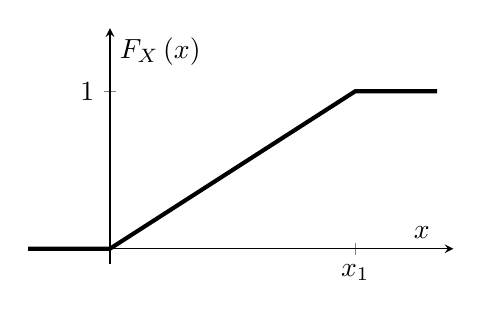
\begin{tikzpicture}
	\begin{axis}[% Cosas comunes a todos los gráficos
		width=5.4cm,height=3cm, scale only axis,
		xmin=-1, xmax=4.2, xlabel={$x$},xtick={0,3},xticklabels={,$x_{1}$,},
		ymin=-0.1, ymax=1.4, ytick={1},
		axis x line=middle,
		x tick label style={{xshift=0pt},{yshift=0pt}}, ylabel=$F_{X}\left( {x} \right)$,yticklabels={$1$},
		x label style={{xshift=-5pt},{yshift=0pt}},
		axis y line=middle]
	 	\draw[line width=1.5pt, color=black] (axis cs:-1,0) --(axis cs:0,0) --  (axis cs:3,1) --  (axis cs:4,1);
	\end{axis}
\end{tikzpicture}  
}% 
\hspace{10pt}% 
\subfloat[][]{% 
\label{fig04-02b}% 
\begin{tikzpicture}
	\begin{axis}[% Cosas comunes a todos los gráficos
		width=5.4cm,height=3cm, scale only axis,
		xmin=-1, xmax=4.2, xlabel={$x$},xtick={0,3},xticklabels={,$x_{1}$},
		ymin=-0.1, ymax=1.4, ytick={1},
		axis x line=middle,
		x tick label style={{xshift=0pt},{yshift=0pt}}, ylabel=$f\xb{X}\left( {x} \right)$,yticklabels={$\dfrac{1}{x_{1}}$},
		x label style={{xshift=-5pt},{yshift=0pt}},
		axis y line=middle]
		\draw[line width=1.5pt, color=black] (axis cs:0,1) -- (axis cs:3,1)-- (axis cs:3,0);  
\end{axis}
\end{tikzpicture}  
}
\caption[Función de distribución y Función densidad de probabilidad de una variable aleatoria continua]{Función de distribución y Función densidad de probabilidad de una variable aleatoria continua.}
\label{fig04-02} 
\end{figure} 

Un ejemplo de cómo se gestionan las tablas que puedan segmentarse a través de más de una página se muestra en la \autoref{tab01-08}, obtenida con el siguiente código:
%
\begin{lstlisting}[frame=none]
\begin{longtable}{p{3.5cm}p{8cm}}
\caption{Funciones de manipulación de gráficos} \label{tab01-08}\\
\hline
{\rule[-8pt]{0pt}{22pt}\bfseries{Función}} & Significado\\
\hline %\rule{0pt}{1pt}
\endfirsthead
\caption[]{..continuación} \\
\hline
{\rule[-8pt]{0pt}{22pt}\bfseries{Función}} & Significado\\
\hline %\rule{0pt}{1pt}
\endhead
\hline
\endfoot %\rule{0pt}{14pt}
\texttt{xlabel('texto')} & Etiqueta el eje \texttt{x} de la gráfica actual\\ 
\texttt{ylabel('texto')} & Etiqueta el eje \texttt{y} de la gráfica actual\\ 
\texttt{title('texto')} & Título de la gráfica actual\\ 
\texttt{text(x,y, 'texto')} & Introduce ``texto'' en la posición \texttt{(x,y)} de la gráfica actual\\ 
\texttt{legend()} & Permite definir rótulos para las distintas líneas o curvas de la gráfica\\ 
\texttt{grid} & Dibuja una rejilla. Con \texttt{grid off} desaparece la cuadrícula\\ 
\texttt{axis([xmin xmax ymin ymax])} & Fija los valores máximos y mínimos de los ejes\\ 
\texttt{axis equal} &Establece que la escala de los ejes sea la misma\\ 
\texttt{axis square} & Fija que la gráfica sea un cuadrado\\ 
\end{longtable}
\end{lstlisting}
%
%
\begin{longtable}{p{3.5cm}p{8cm}}
\caption{Funciones de manipulación de gráficos} \label{tab01-08}\\
\hline
{\rule[-8pt]{0pt}{22pt}\bfseries{Función}} & Significado\\
\hline %\rule{0pt}{1pt}
\endfirsthead
\caption[]{..continuación} \\
\hline
{\rule[-8pt]{0pt}{22pt}\bfseries{Función}} & Significado\\
\hline %\rule{0pt}{1pt}
\endhead
\hline
\endfoot %\rule{0pt}{14pt}
\texttt{xlabel('texto')} & Etiqueta el eje \texttt{x} de la gráfica actual\\ 
\texttt{ylabel('texto')} & Etiqueta el eje \texttt{y} de la gráfica actual\\ 
\texttt{title('texto')} & Título de la gráfica actual\\ 
\texttt{text(x,y, 'texto')} & Introduce ``texto'' en la posición \texttt{(x,y)} de la gráfica actual\\ 
\texttt{legend()} & Permite definir rótulos para las distintas líneas o curvas de la gráfica\\ 
\texttt{grid} & Dibuja una rejilla. Con \texttt{grid off} desaparece la cuadrícula\\ 
\texttt{axis([xmin xmax ymin ymax])} & Fija los valores máximos y mínimos de los ejes\\ 
\texttt{axis equal} &Establece que la escala de los ejes sea la misma\\ 
\texttt{axis square} & Fija que la gráfica sea un cuadrado\\ 
\end{longtable}

\subsection{Gestión de índices alfabéticos y glosario}
Para gestionar el índice alfabético se ha utilizado el paquete \ttcolorc{imakeidx}\index{imakeidx}. Se ha optado por generar un índice alfabético con tres columnas y con una letra antes de cada grupo de palabras del índice. Para ello se ha redefinido el entorno \ttcolor{theindex}\index{theindex}.

Para incluir algo en el índice el comando standard es \ttcolorc{index} y además se han creado un par de comandos: el comando \ttcolorc{indexit} que pone la palabra correspondiente en cursiva y además se incluye en el índice y \ttcolorc{ind} que es idéntica a \ttcolorc{index}.

Para los glosarios se utiliza el paquete \ttcolor{glossaries}\index{glossaries} cuyo uso ya ha sido explicado.

\subsection{Ajustes en fórmulas}
La escritura de fórmulas en \LaTeX\ requiere el conocimiento de un conjunto de comandos que se encuentran muy bien explicados en el documento \ttcolor{mathmode.pdf}. Uno de los comandos que facilitan esta escritura y algunos efectos especiales se basan en el uso de los paquetes \ttcolor{cancel}\index{cancel} y \ttcolor{kbordermatrix}\index{kbordermatrix}. Para permitir la escritura de matrices con diferentes limitadores, hemos utilizado el paquete \ttcolor{array}\index{array}.

Debido a un bug de  \LuaLaTeX\ es necesario escribir fórmulas demasiado anchas mediante el entorno \comando{begin\{equationw\}}\index{equationw}. Un ejemplo se muestra a continuación y el resultado del mismo posteriormente.

\begin{LTXexample}[pos=b, hsep=15pt,width=\textwidth]
\begin{equationw}
\E\left[ {Y} \right]=\E\left[ {\left( {X-m_{X}} \right)^{n}} \right]=\begin{cases}
1\times 3 \times \cdots \times \left( {2k-1} \right)\sigma_{X}^{2k}=\frac{\left( {2k} \right)!\sigma_{X}^{2k}}{2^{k}k!}&\textrm{ para }n=2k \\
0 &\textrm{ para }n=2k +1
\end{cases}
\end{equationw}
\end{LTXexample}
Podemos observar la posición del número de ecuación que se ha desplazado debajo de la fórmula. Para crear el entorno que ha permitido resolver este error (el número de ecuación se desplazaba a la derecha), ha sido necesario cargar el paquete \ttcolor{environ}.

También para corregir otro bug de \LuaLaTeX\ hemos introducido el comando \ttcolorc{sqrtlua}\index{sqrtlua} que evita el desplazamiento del contenido bajo el signo de la raíz cuando dicho contenido tiene una altura superior a un renglón. Esta definición hay que encontrarla en el bloque de gestión de fuentes.

\subsection{Hiperenlaces}\index{hyperref}

La creación de los hiperenlaces en los documentos escritos en \LaTeX\ se gestiona mediante el paquete \ttcolor{hyperref}. La documentación de este paquete es extensa y muy detallada y permite, por ejemplo, manejar con facilidad los colores de los hiperenlaces, la utilización de comandos inteligentes como \ttcolorc{autoref}\index{autores}, etc. 

El ajuste más genérico de \ttcolor{hyperref} se ha realizado en esta hoja de estilo pero adicionalmente se han definido otros ajustes en el fichero principal de manera que, por ejemplo, se generen ficheros pdf con palabras claves que les permitan ser localizados con los buscadores, como podemos ver en la líneas de código siguientes:

\begin{lstlisting}[frame=none]
\hypersetup
	{
 	linkcolor=black, %Tocar para poner color en enlaces
	pdfauthor={\elautor},
	pdftitle={\eltitulo}, 
	citecolor=black, %Tocar para poner color en enlaces, eg blue
	pdfkeywords={Formato de Libro para la ETSI, Universidad de Sevilla}	
	 }
\end{lstlisting}
  
Dentro de este apartado, mencionar la utilización de los paquetes \ttcolor{zref-lastpage} y \ttcolor{zref-user}\index{zref-lastpage}\index{zref-user} para detectar el número total de páginas de un documento, que viene dado por \comandos{zpageref}{Lastpage}, o bien el ajuste que se realiza sobre las direcciones url, del paquete \ttcolor{url}\index{url}, que ha sido cargado automáticamente.

\subsection{Listado de códigos}
Es habitual en textos escritos en la Escuela el uso de listados de códigos de muy diversa índole. Nosotros hemos elegido el paquete \ttcolor{listings}\index{listings} para gestionarlos en nuestros documentos. Este paquete se encuentra perfectamente documentado, lo que nos ha permitido realizar algunos ajustes que hemos considerado necesarios. 

En el caso de utilizar \LaTeX\ es necesario que los símbolos no habituales se declaren, como hemos hecho en el siguiente bloque:
\begin{lstlisting}[frame=none]
\ifluatex
\else
\lstset{literate=%
    {á}{{\'a}}1
    {é}{{\'e}}1
    {í}{{\'i}}1
    {ó}{{\'o}}1
    {ú}{{\'u}}1
    {Á}{{\'A}}1
    {É}{{\'E}}1
    {Í}{{\'I}}1
    {Ó}{{\'O}}1
    {Ú}{{\'U}}1
    {ñ}{{\~{n}}}1
    {º}{{\textsuperscript{\b{o}}}}1
    {ª}{{\textsuperscript{\b{a}}}}1
    {¿}{{?`}}1
}
\fi
\end{lstlisting}
%
Y también hemos tenido que ajustar determinados problemas relacionados con el uso de los idiomas español e inglés.  Por último, hemos ajustado el ``caption'' de los códigos mediante la declaración de un formato y modificado ligeramente la manera en la que se realiza el listado de los mismos, mediante el siguiente conjunto de instrucciones.
 
\begin{lstlisting}[frame=none]
\makeatletter
	\renewcommand*{\l@lstlisting}[2]{\@dottedtocline{1}{.1em}{2.8em}{\tocsecc #1}{\tocsecc #2}}
\makeatother
\end{lstlisting}

\subsection{Entornos, teoremas y similares}
En este apartado hemos agrupado un conjunto de paquetes relacionados con la creación de entornos específicos y estructuras como los teoremas y elementos similares.

En primer lugar, utilizamos el paquete \ttcolor{mdframed}\index{mdframed} para poder crear cajas sombreadas que se continúan a través de más de una página. Aunque no se ha utilizado en este estilo, merece señalarse la existencia del paquete \ttcolor{tcolorbox}\index{tcolorbox} que permite una gestión probablemente más flexible con este mismo fin.

A continuación, señalamos la creación del entorno \ttcolor{Resumen} que permite realizar resúmenes en el lugar del texto que nos interese, como ya hemos mencionado y mostrado en un apartado anterior.

Para la gestión de los teoremas y elementos similares hemos escogido el paquete \ttcolor{ntheorem}\index{ntheorem} junto con una serie de opciones. Si analizamos las siguientes líneas de código, en la que se define el entorno \ttcolor{teor}:

\begin{lstlisting}[frame=none, numbers=left, xleftmargin=2em]
\theoremnumbering{arabic}
\theoremheaderfont{\aheadteoremas}
\theoremseparator{\hspace{.2em}}
\theorembodyfont{\itshape}
\newtheorem{teor}{\theoremname}[section]
\end{lstlisting}

Podemos observar que el la línea \ttcolor{1} el esquema de numeración será arábico, esto es, mediante números. Para su declaración utilizaremos el comando \comando{aheadteoremas} que habíamos definido anteriormente y nos indica que utilizaremos una determinada fuente con las características que habíamos señalado. El enunciado del teorema irá en \emph{cursiva} y el nombre que usaremos viene marcado por el macro  \comando{theoremname}. Por último, al incluir el término \ttcolor{section} en la línea \ttcolor{5} estamos señalando que la numeración de los teoremas se realizará al nivel de sección; esto es, las siguientes líneas de código, en las que también hemos utilizado el entorno \ttcolor{demo}, generan el teorema debajo de las mismas.

%\begin{LTXexample}[pos=b, hsep=15pt,width=\textwidth]
\begin{lstlisting}[frame=none]
\begin{teor}\label{th04-02} Si una función $f\left( {x} \right)$ tiene una segunda derivada que es no negativa (positiva) en un intervalo dado, la función es convexa (estrictamente convexa) en ese intervalo.
\end{teor}
\begin{demo} Para probar el teorema, desarrollemos la función en serie de Taylor alrededor del punto $x_{0}$:
\begin{equation}\label{eq04-321}
f\left( {x} \right)=f\left( {x_{0}} \right)+f^{\prime}\left( {x_{0}} \right)\left( {x-x_{0}} \right)+\frac{f^{\prime \prime}\left( {x^{\ast}} \right)}{2}\left( {x-x_{0}} \right)^{2}
\end{equation}
donde $x^{\ast}$ está entre $x_{0}$ y $x$. Por hipótesis, $f^{\prime \prime}\left( {x^{\ast}} \right)\ge 0$, así que el último término es no negativo para todo $x$.

...
\end{demo}
\end{lstlisting}
%\end{LTXexample}

\begin{teor}\label{th04-02} Si una función $f\left( {x} \right)$ tiene una segunda derivada que es no negativa (positiva) en un intervalo dado, la función es convexa (estrictamente convexa) en ese intervalo.
\end{teor}
\begin{demo} Para probar el teorema, desarrollemos la función en serie de Taylor alrededor del punto $x_{0}$:
\begin{equation}\label{eq04-321}
f\left( {x} \right)=f\left( {x_{0}} \right)+f^{\prime}\left( {x_{0}} \right)\left( {x-x_{0}} \right)+\frac{f^{\prime \prime}\left( {x^{\ast}} \right)}{2}\left( {x-x_{0}} \right)^{2}
\end{equation}
donde $x^{\ast}$ está entre $x_{0}$ y $x$. Por hipótesis, $f^{\prime \prime}\left( {x^{\ast}} \right)\ge 0$, así que el último término es no negativo para todo $x$.

...
\end{demo}

Existen un conjunto de entornos definidos de manera análoga al anterior y su uso puede ser fácilmente deducible del ejemplo anterior.

\subsection{Otros comandos}
Finalizamos la descripción del fichero señalando la existencia de un grupo de comandos muchos de ellos únicamente utilizables en la escritura de un texto como el presente. Otros, como las definiciones de las cabeceras de los exámenes o el que nos permite crear una dedicatoria de nuestro texto. Ambos se gestionan en el fichero principal con líneas de código similares a las siguientes:

\begin{lstlisting}[frame=none]
\dedicatoria{A nuestras familias\\A nuestros maestros} 
\titulacion{ Grado en Ingeniería de Tecnología de Telecomunicación}
\asignatura{Comunicaciones Digitales}
\convocatoria{Primera convocatoria. Curso 2013-14}
\fecha{3/02/2014}
\end{lstlisting}
%
con el resultado que ya hemos mostrado.

\section{A modo de conclusión}
Hemos tratado de mostrar en este capítulo los elementos más destacados del diseño de la hoja de estilo que hemos realizado para nuestra Escuela. Como hemos dicho con anterioridad, hay mucho de gusto personal en el diseño pero también existe un considerable compromiso con tendencias actuales en la maquetación de textos científicos. 

Como todo diseño, es manifiestamente mejorable y nuestro deseo es que este capítulo permita a quien lo desee adaptarla a sus criterios. Tenemos intención de crear una página de preguntas y respuestas que permitan, con la aportación de todos, mejorar esta primera aportación a la creación de una imagen corporativa de los documentos generados en nuestra Escuela.

 



 
 %:Empezamos con los apéndices, que irían en uno o más ficheros. Es necesario incluir estos ficheros entre el entorno \begin{appendices}....\end{appendices} debido a que se ha deseado utilizar un formato diferente para el título de los apéndices, incluyendo la palabra apéndice, para la numeración de los apéndices, alfabético, y para las cabeceras de las páginas.

\begin{appendices}
% Fichero en el que se incluyen los apéndices
% !TEX root =../LibroTipoETSI.tex



%APENDICE A
\chapter{Aerodinámica potencial 2D. Método de Green.}\LABAPEN{ApA}

%\Blindtext


%%%%%%%%%%%%%%%%%%%%%%%%%%%%%%%%%%%%%%%
%APENDICE B
\chapter{Aerodinámica de alas de envergadura finita. Vortex-Lattice}\LABAPEN{ApB}

 %Ver este fichero para incluir ahí los apéndices.
\end{appendices}
%:Fin de la inclusión de apéndices

%:Empieza todo lo que no constituye el cuerpo en si del libro. Todo lo que va detrás
\backmatter

%:Indice de figuras, coméntese las siguientes líneas si no se desea
\cleardoublepage
\phantomsection

%:Para añadir una línea en blanco en el TOC y separar esta lista
\addtocontents{toc}{\protect\mbox{}\protect\hspace*{0pt}\par}
\addcontentsline{toc}{listasb}{\listfigurename}
\pagestyle{especial}
\listoffigures

%:Indice de tablas, coméntese las siguientes líneas si no se desea
\cleardoublepage
\phantomsection
\addcontentsline{toc}{listasb}{\listtablename}
\pagestyle{especial}
\listoftables

%:Indice de Programas
\cleardoublepage
\phantomsection
\addcontentsline{toc}{listasb}{\lstlistlistingname}
\pagestyle{especial}
\lstlistoflistings

%:Bibliografía con biblatex y biber
\cleardoublepage
\phantomsection
\addcontentsline{toc}{listasb}{\bibname}
\pagestyle{especial}
%BIBER
%\printbibliography[heading=etsi]
%BIBTEX
%\bibliographystyle{IEEEtran}
\bibliographystyle{amsplain} %flexbib amsplain alpha
%:Fichero con la bibliografía, BIBTEX
\bibliography{bibliografiaLibroETSI}

%:Índice alfabético
\cleardoublepage
\phantomsection
\addcontentsline{toc}{listasb}{\indexname}
\chaptermark{\indexname}
\printindex

%:Acrónimos
\cleardoublepage
\phantomsection
\addcontentsline{toc}{listasb}{\glossaryname}
\chaptermark{\glossaryname}
\printglossaries

\end{document}